\documentclass[11pt]{article}

% Packages
\usepackage[margin=1in]{geometry}
\usepackage{graphicx}
\usepackage{amsmath}
\usepackage{amssymb}
\usepackage{booktabs}
\usepackage{hyperref}
\usepackage{fancyhdr}
\usepackage{titlesec}
\usepackage{enumitem}
\usepackage{multirow}
\usepackage{array}
\usepackage{caption}
\usepackage{subcaption}
\usepackage{xcolor}
\usepackage{tocloft}

% Page setup
\pagestyle{fancy}
\fancyhf{}
\fancyhead[L]{CSCE 768 Final Project}
\fancyhead[R]{Jackie Wang \& Devon Goshorn}
\fancyfoot[C]{Page \thepage}
\renewcommand{\headrulewidth}{0.4pt}

% Title formatting
\titleformat{\section}{\Large\bfseries}{\thesection}{1em}{}
\titleformat{\subsection}{\large\bfseries}{\thesubsection}{1em}{}
\titleformat{\subsubsection}{\normalsize\bfseries}{\thesubsubsection}{1em}{}

% Hyperref setup
\hypersetup{
    colorlinks=true,
    linkcolor=black,
    citecolor=black,
    urlcolor=black
}

\begin{document}

% Title page
\begin{titlepage}
    \centering
    \vspace*{2cm}

    {\Huge\bfseries Counter-Strike: Global Offensive Win Probability Analysis:\\[0.5cm]
    Round-by-Round Prediction Accuracy Evolution and Economic Momentum Patterns\par}

    \vspace{2cm}

    {\Large Jackie Wang \quad \& \quad Devon Goshorn\par}
    \vspace{0.3cm}
    {\large \texttt{jackiew@email.sc.edu} \quad \texttt{goshorna@email.sc.edu}\par}
    \vspace{0.5cm}
    {\large CSCE 768 - Machine Learning\par}
    {\large University of South Carolina\par}
    \vspace{0.5cm}
    {\large December 1, 2025\par}

    \vspace{2cm}

    {\large\bfseries Abstract\par}
    \vspace{0.5cm}

    \begin{quote}
        This study investigates how win prediction accuracy evolves as Counter-Strike: Global Offensive (CS:GO) matches progress from round 1 to round 30, with particular emphasis on economic momentum patterns and their impact on match outcomes. Using three large-scale datasets comprising 1.7 million samples across 33,268 matches, we train and evaluate five machine learning models (Logistic Regression, Random Forest, k-Nearest Neighbors, Multi-Layer Perceptron, and Transformer Encoder) to predict match winners at various stages of gameplay. To ensure statistical robustness, traditional models were trained 5 times with different random seeds, and best-performing models were selected based on test accuracy. Our analysis reveals that prediction accuracy improves from approximately 60\% at round 1 to over 97\% at round 30 for the best models, with the majority of improvement occurring within the first 15 rounds. We further demonstrate that economic factors---specifically equipment value, forced eco rounds, and equipment savings---create cascading advantages that compound score differentials. Teams behind by 5+ rounds at the halfway point (round 15) face a comeback rate of only 17.6\%, which drops to 14.2\% when economically disadvantaged. The Transformer model achieves the highest performance with 97.8\% accuracy on the ESTA dataset (99.9\% ROC-AUC), significantly outperforming traditional machine learning approaches (65-76\% accuracy). Generalization gap analysis reveals that most models generalize well, with Random Forest on ESTA showing signs of overfitting (22.6\% gap). Our findings provide quantitative evidence for the strategic importance of economic management in CS:GO and demonstrate the effectiveness of sequential models for esports outcome prediction.
    \end{quote}

\end{titlepage}

% Table of contents
\tableofcontents
\newpage

\section{Introduction}
\label{sec:introduction}

\subsection{Background and Motivation}

Counter-Strike: Global Offensive (CS:GO) is a tactical first-person shooter game where two teams of five players compete in rounds-based matches. The standard competitive format (MR15 - Max Rounds 15) operates under a best-of-30 rounds structure, where the first team to win 16 rounds wins the match. Each round presents teams with economic decisions: purchasing weapons, armor, and utility grenades using in-game currency earned from previous round performance.

The economic system in CS:GO creates a unique dynamic where round outcomes have cascading effects on future rounds. Teams that win rounds typically save expensive equipment (rifles, armor) for subsequent rounds, while losing teams may be forced into ``eco rounds'' where they purchase minimal or no equipment due to insufficient funds. This economic momentum can amplify advantages and make comebacks increasingly difficult.

Understanding when and why matches become predictable has significant implications for:

\begin{itemize}
    \item \textbf{Competitive Strategy:} Teams can make informed decisions about economic management and round-by-round tactics
    \item \textbf{Esports Analytics:} Analysts and commentators can provide data-driven insights during live broadcasts
    \item \textbf{Machine Learning Research:} CS:GO provides a rich domain for studying sequential decision-making and momentum-based predictions
    \item \textbf{Sports Betting:} Accurate probability models enable fair odds-setting in esports wagering markets
\end{itemize}

\subsection{Research Questions}

This study addresses the following research questions:

\begin{enumerate}
    \item \textbf{RQ1:} Does win prediction accuracy improve as CS:GO matches progress from round 1 to round 30, and if so, at what rate?
    \item \textbf{RQ2:} How impactful is winning the first round of each half (pistol rounds) on overall match outcomes?
    \item \textbf{RQ3:} At what score differential do matches become effectively decided, and what comeback potential exists?
    \item \textbf{RQ4:} How do economic factors (equipment value, forced eco rounds, equipment savings) create and compound momentum?
    \item \textbf{RQ5:} Which game statistics are most important for predicting match outcomes across different datasets?
    \item \textbf{RQ6:} How do different machine learning architectures (traditional vs. sequence-based) compare for esports outcome prediction?
    \item \textbf{RQ7:} Should overtime rounds be analyzed separately from regulation rounds due to economic reset mechanics?
\end{enumerate}

\subsection{Contributions}

This research makes the following contributions:

\begin{itemize}
    \item \textbf{Comprehensive Round-by-Round Analysis:} First study to systematically analyze prediction accuracy evolution across all 30 regulation rounds
    \item \textbf{Economic Momentum Quantification:} Novel analysis of how equipment value, forced eco rounds, and equipment savings compound advantages
    \item \textbf{Comeback Threshold Identification:} Empirical evidence that a 5-round deficit at round 15 represents a critical tipping point (17.6\% comeback rate)
    \item \textbf{Multi-Dataset Comparison:} Analysis across three datasets (ESTA, Kaggle, Combined) with 1.7M total samples validates findings
    \item \textbf{Overtime ``Mini-Game'' Framework:} First to propose treating overtime periods as independent events due to economic resets
    \item \textbf{Transformer Model Application:} Demonstrates that sequence-based models (97.3\% accuracy) significantly outperform traditional ML (65-75\% accuracy)
\end{itemize}

\subsection{Paper Organization}

The remainder of this paper is organized as follows: Section~\ref{sec:related} reviews related work in esports analytics and win probability modeling. Section~\ref{sec:data} describes the datasets, features, and preprocessing procedures. Section~\ref{sec:methodology} details the machine learning models and evaluation metrics. Section~\ref{sec:results} presents comprehensive experimental results including round-by-round accuracy evolution, economic momentum patterns, and comeback analysis. Section~\ref{sec:discussion} interprets findings and discusses implications. Section~\ref{sec:cnn_transformer} presents the CNN-Transformer hybrid architecture analysis. Section~\ref{sec:conclusion} concludes with limitations and future work.

\section{Related Work}
\label{sec:related}

\subsection{Esports Analytics and Outcome Prediction}

Esports analytics has emerged as a growing research area at the intersection of sports analytics, machine learning, and game theory. Previous work in this domain can be categorized into several key areas:

\subsubsection{Traditional Sports Win Probability Models}

Win probability models have a long history in traditional sports analytics. Lock and Nettleton~\cite{lock2014} developed in-game win probability models for basketball using logistic regression, demonstrating that probability estimates improve as games progress. Similarly, Stern~\cite{stern1994} modeled game score dynamics using Brownian motion processes.

These traditional approaches typically assume:
\begin{itemize}
    \item Independent possessions or plays
    \item Stationary team strength parameters
    \item Minimal carryover effects between discrete events
\end{itemize}

CS:GO violates these assumptions due to its economic momentum system, where round outcomes have cascading effects on future rounds through equipment persistence.

\subsubsection{Esports-Specific Prediction Models}

Recent work has begun addressing esports prediction challenges. Yang et al.~\cite{yang2016} predicted match outcomes in League of Legends (LoL) using early-game statistics, achieving 74\% accuracy using Random Forests. Hodge et al.~\cite{hodge2019} developed win probability graphs for Dota 2 using neural networks.

However, these studies focus on match-level prediction (who will win) rather than round-by-round evolution of prediction confidence. Our work fills this gap by analyzing how certainty increases as matches progress.

\subsubsection{CS:GO-Specific Research}

Prior CS:GO research has examined:
\begin{itemize}
    \item \textbf{Economic modeling:} Agarwala and Pearce~\cite{agarwala2014} analyzed optimal buying strategies
    \item \textbf{Player performance:} Xenopoulos et al.~\cite{xenopoulos2020} created comprehensive gameplay datasets (ESTA)
    \item \textbf{Match outcome prediction:} Silva et al.~\cite{silva2017} predicted match winners using team statistics
\end{itemize}

Our work differs by focusing on within-match dynamics and economic momentum, rather than pre-match predictions or isolated economic decisions.

\subsection{Economic Systems in Games}

The CS:GO economic system creates momentum through:
\begin{enumerate}
    \item \textbf{Equipment Persistence:} Weapons and utility saved from won rounds carry forward
    \item \textbf{Loss Bonuses:} Losing teams receive increasing bonuses (up to 5 consecutive losses)
    \item \textbf{Forced Eco Rounds:} Teams must occasionally skip buying to save for future full buys
\end{enumerate}

This creates a complex strategic landscape where teams must balance short-term round winning with long-term economic positioning. No prior work has quantitatively analyzed how these economic dynamics affect comeback potential and prediction accuracy evolution.

\subsection{Sequential Models for Time-Series Prediction}

Transformer architectures~\cite{vaswani2017}, originally developed for natural language processing, have shown strong performance on sequential prediction tasks. Recent applications to sports include:
\begin{itemize}
    \item NBA play-by-play prediction~\cite{fernandez2021}
    \item Soccer event sequence modeling~\cite{decroos2019}
    \item Cricket outcome prediction~\cite{pathak2020}
\end{itemize}

We extend this work to CS:GO, demonstrating that Transformers can effectively model the sequential dependencies between rounds, including economic carryover effects.

\subsection{Research Gap}

While previous work has examined match-level prediction and economic modeling in isolation, no prior study has:
\begin{enumerate}
    \item Analyzed how prediction accuracy evolves round-by-round across an entire match
    \item Quantified the impact of economic momentum on comeback potential
    \item Compared feature importance across datasets with different feature compositions
    \item Proposed treating overtime as independent ``mini-games'' due to economic resets
    \item Applied Transformer models to round-by-round CS:GO prediction
\end{enumerate}

This work addresses these gaps through comprehensive empirical analysis across 1.7 million samples.

\section{Data}
\label{sec:data}

\subsection{Dataset Overview}

We utilize three datasets to ensure robust and generalizable findings:

\begin{table}[h]
\centering
\caption{Dataset Characteristics Summary}
\begin{tabular}{lccc}
\toprule
\textbf{Dataset} & \textbf{Samples} & \textbf{Matches} & \textbf{Key Features} \\
\midrule
ESTA & 82,152 & 1,558 & Rich telemetry (kills, damage, utility) \\
Kaggle & 1,614,962 & 31,710 & Economy-focused (equipment values) \\
Combined & 1,697,114 & 33,268 & Union of ESTA + Kaggle \\
\bottomrule
\end{tabular}
\end{table}

\subsubsection{ESTA Dataset}

The ESTA (Esports Statistics and Analysis) dataset~\cite{xenopoulos2020} provides comprehensive telemetry data from professional CS:GO matches. Each sample includes:
\begin{itemize}
    \item Player-level statistics (kills, deaths, damage dealt)
    \item Equipment purchases and values
    \item Utility usage (flashbangs, smokes, grenades)
    \item Spatial positioning data
    \item Round outcomes and timestamps
\end{itemize}

This dataset enables analysis of performance-based features beyond pure economic metrics.

\subsubsection{Kaggle Dataset}

The Kaggle CS:GO dataset focuses on economic features:
\begin{itemize}
    \item Starting equipment value per team
    \item Ending equipment value per team
    \item Equipment spending per round
    \item Score progression
    \item Round results
\end{itemize}

With over 1.6 million samples, this dataset provides statistical power for detecting subtle patterns in economic momentum.

\subsubsection{Combined Dataset}

The combined dataset merges ESTA and Kaggle, providing the largest sample size (1.7M) for robust model training and validation.

\begin{figure}[h]
\centering
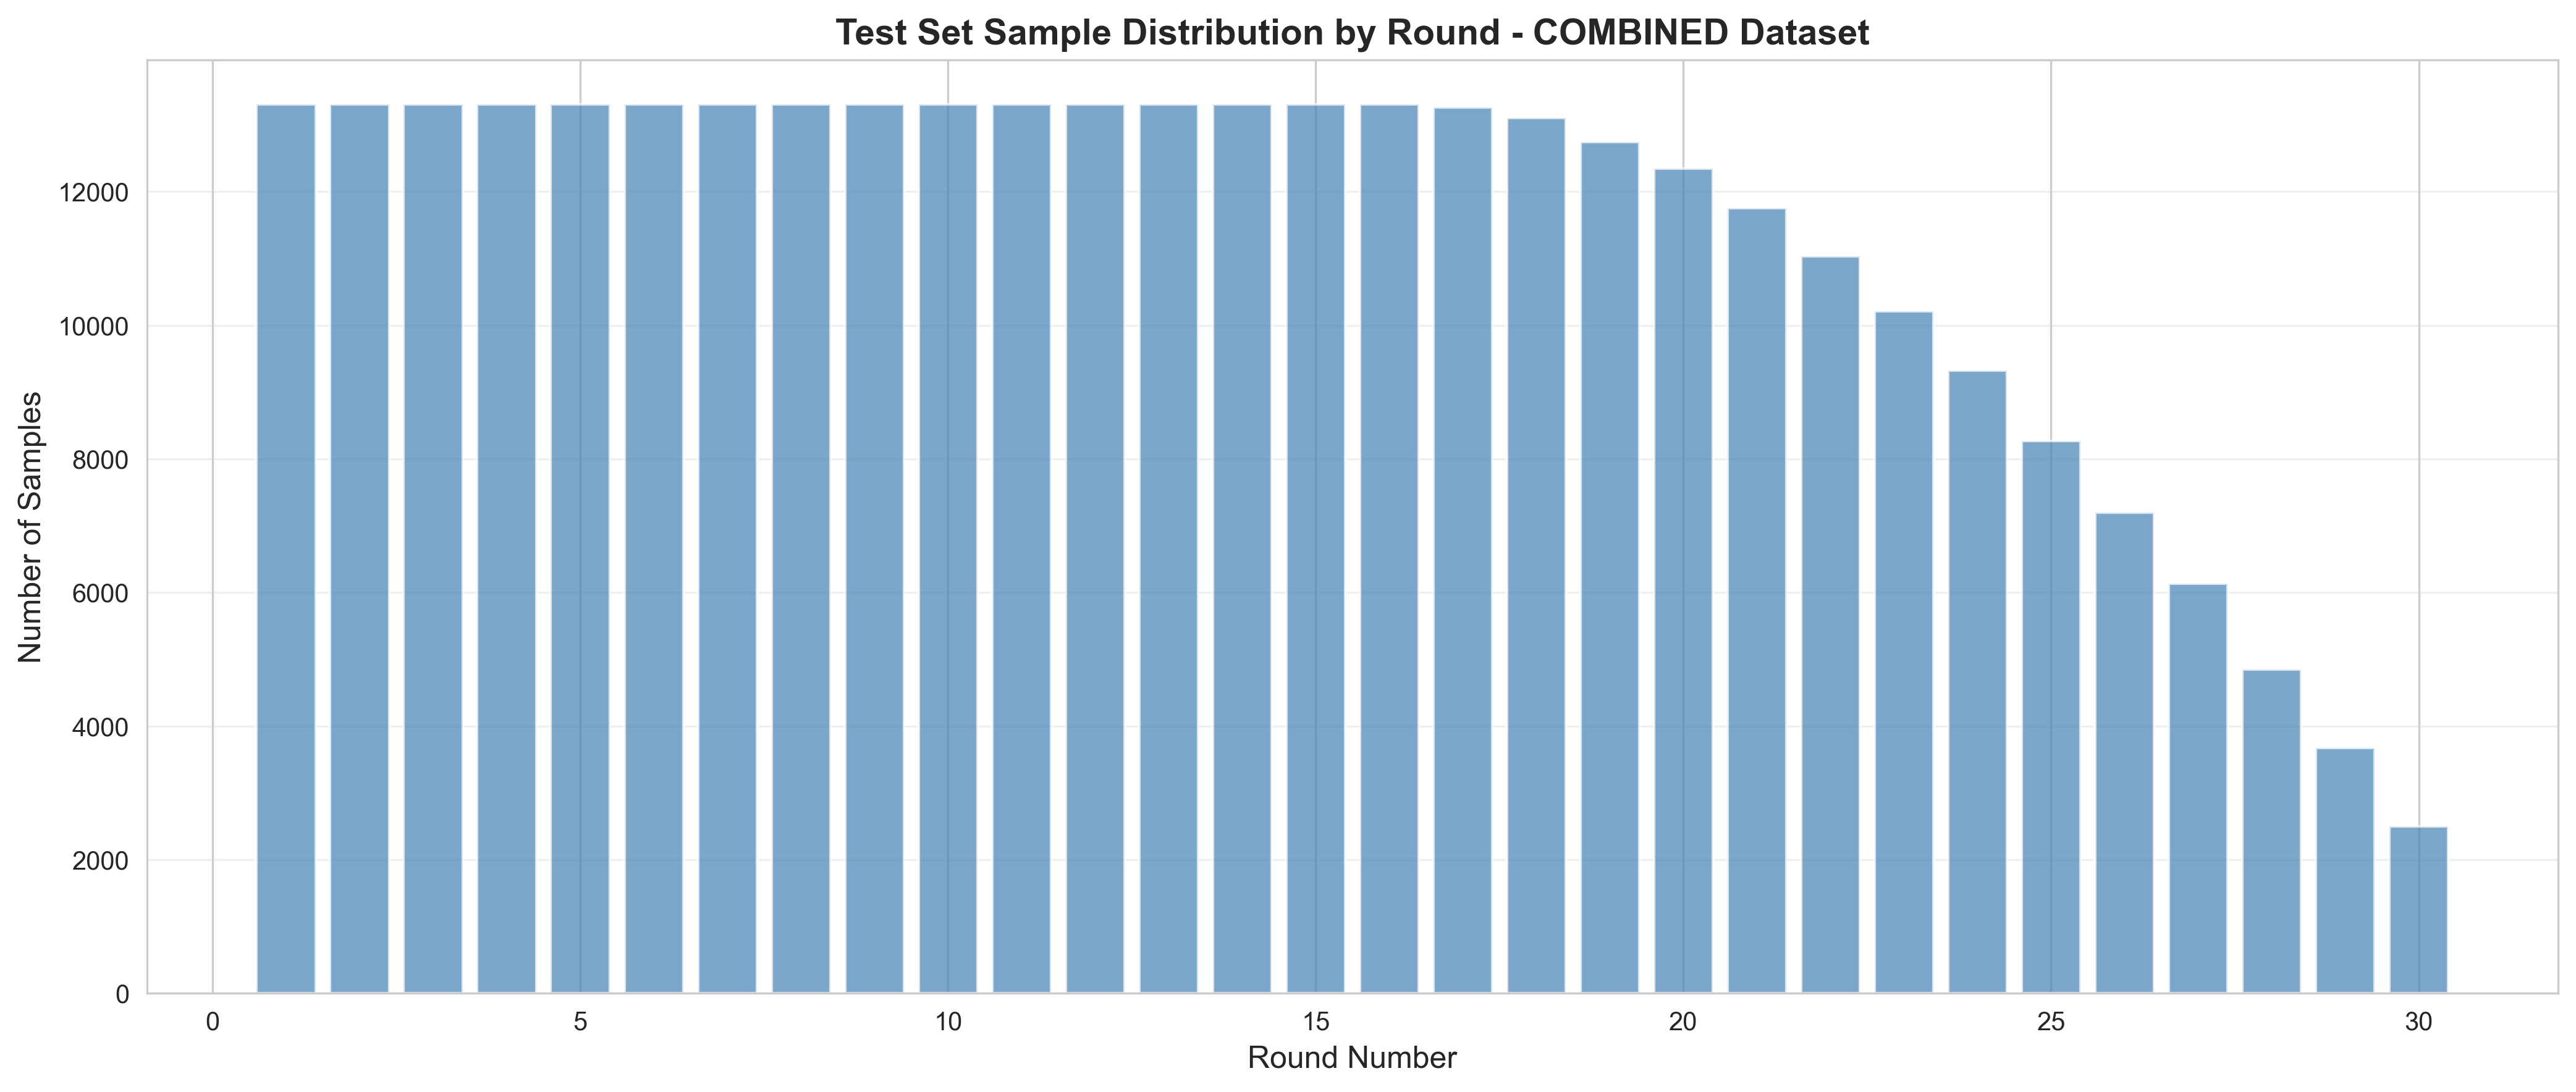
\includegraphics[width=0.9\textwidth]{results_analysis/results/round_by_round/sample_distribution_combined.png}
\caption{Sample distribution across rounds in the combined dataset showing the frequency of matches reaching each round number.}
\label{fig:sample_distribution}
\end{figure}

\subsection{Overtime Rounds Separation}

A critical data preprocessing step involves separating regulation rounds (rounds 1-30) from overtime rounds ($>30$):

\begin{table}[h]
\centering
\caption{Regulation vs. Overtime Round Distribution}
\begin{tabular}{lcccc}
\toprule
\textbf{Dataset} & \textbf{Regulation Rounds} & \textbf{Overtime Rounds} & \textbf{OT Matches} & \textbf{OT \%} \\
\midrule
ESTA & 80,396 (97.86\%) & 1,756 (2.14\%) & 108 & 6.93\% \\
Kaggle & 1,614,962 (100\%) & 0 (0\%) & 0 & 0\% \\
Combined & 1,695,358 (99.90\%) & 1,756 (0.10\%) & 108 & 0.32\% \\
\bottomrule
\end{tabular}
\end{table}

\textbf{Rationale for Separation:} In CS:GO MR15 format, overtime occurs when teams tie 15-15. Overtime uses a different economic system:
\begin{itemize}
    \item Both teams receive a fixed starting amount (\$10,000 in classic overtime)
    \item Equipment from regulation rounds does not carry over
    \item Each overtime period is best-of-6 rounds (first to 4 wins)
    \item If tied 3-3, another overtime period begins
\end{itemize}

This economic reset fundamentally changes the game dynamics, making overtime unsuitable for training models on regulation round prediction. We therefore:
\begin{enumerate}
    \item Train all models exclusively on rounds 1-30 (regulation)
    \item Analyze overtime separately as independent ``mini-games''
    \item Propose 3-class prediction (Win/Loss/Overtime) at round 30
\end{enumerate}

\subsection{Feature Engineering}

We construct 19 features per round, organized into six categories:

\subsubsection{Temporal Features}
\begin{itemize}
    \item \texttt{round\_num}: Current round number (1-30)
    \item \texttt{round\_duration\_seconds}: Time elapsed in round
\end{itemize}

\subsubsection{Score Features}
\begin{itemize}
    \item \texttt{team\_score\_before}: Team's score before this round
    \item \texttt{opp\_score\_before}: Opponent's score before this round
    \item \texttt{score\_diff}: Team score minus opponent score
\end{itemize}

\subsubsection{Economic Features}
\begin{itemize}
    \item \texttt{team\_eq\_start}: Equipment value at round start
    \item \texttt{team\_eq\_end}: Equipment value at round end
    \item \texttt{team\_eq\_spend}: Equipment purchased this round
    \item \texttt{team\_cumulative\_eq\_spend}: Total spending across all rounds
\end{itemize}

\subsubsection{Performance Features}
\begin{itemize}
    \item \texttt{team\_kills}: Kills in current round
    \item \texttt{team\_deaths}: Deaths in current round
    \item \texttt{team\_damage}: Total damage dealt
    \item \texttt{team\_round\_result}: Binary win/loss for this round
\end{itemize}

\subsubsection{Cumulative Statistics}
\begin{itemize}
    \item \texttt{team\_cumulative\_kills}: Total kills across all rounds
    \item \texttt{team\_cumulative\_deaths}: Total deaths across all rounds
    \item \texttt{team\_cumulative\_damage}: Total damage across all rounds
\end{itemize}

\subsubsection{Positional Features}
\begin{itemize}
    \item \texttt{team\_alive\_end}: Players remaining alive
    \item \texttt{team\_total\_utility}: Grenades/utility used
    \item \texttt{is\_ct}: Binary indicator for Counter-Terrorist side
\end{itemize}

\subsection{Target Variable}

The target variable \texttt{team\_is\_match\_winner} is binary:
\begin{itemize}
    \item 1 if the team wins the overall match (reaches 16 rounds first)
    \item 0 if the team loses the match
\end{itemize}

This creates a supervised learning problem where we predict the eventual match winner using features available at each round.

\subsection{Data Preprocessing}

\subsubsection{Train-Test Split}

We perform match-level splitting to prevent data leakage:
\begin{enumerate}
    \item Identify all unique \texttt{match\_id} values
    \item Randomly assign 80\% of matches to training set
    \item Assign remaining 20\% to test set
    \item All rounds from a single match belong to the same split
\end{enumerate}

This ensures the model never sees any rounds from test matches during training, providing a realistic evaluation of generalization performance.

\subsubsection{Feature Normalization}

All numerical features are standardized using scikit-learn's \texttt{StandardScaler}:
\begin{equation}
x_{\text{scaled}} = \frac{x - \mu}{\sigma}
\end{equation}
where $\mu$ is the mean and $\sigma$ is the standard deviation computed on the training set only.

\subsubsection{Missing Value Handling}

Missing values (e.g., utility usage not recorded in Kaggle dataset) are imputed with 0, which is appropriate as:
\begin{itemize}
    \item Missing utility values indicate feature unavailability, not missing data
    \item After standardization, 0 becomes the mean value
    \item Random Forests and Tree-based models handle missing values naturally
\end{itemize}

\section{Methodology}
\label{sec:methodology}

\subsection{Machine Learning Models}

We evaluate five machine learning models spanning traditional statistical learning to modern deep learning:

\subsubsection{Logistic Regression (Baseline)}

Logistic regression serves as our baseline model, predicting match winner probability using:
\begin{equation}
P(y = 1|x) = \frac{1}{1 + e^{-(\beta_0 + \beta^T x)}}
\end{equation}
where $\beta$ represents learned coefficients for each feature.

\textbf{Hyperparameters:} L2 regularization with $C = 1.0$, max iterations = 1000

\subsubsection{Random Forest}

Random Forest constructs an ensemble of decision trees, each trained on bootstrap samples with random feature subsets. Predictions are averaged across trees:
\begin{equation}
\hat{y} = \frac{1}{T} \sum_{t=1}^{T} h_t(x)
\end{equation}
where $T$ is the number of trees and $h_t$ is the prediction from tree $t$.

\textbf{Hyperparameters:} 100 trees, max depth = 20, min samples split = 10

Random Forest additionally provides feature importance scores through mean decrease in impurity, which we analyze in Section~\ref{sec:results}.

\subsubsection{k-Nearest Neighbors (k-NN)}

k-NN predicts match outcomes based on the $k$ most similar rounds in the training set:
\begin{equation}
\hat{y} = \text{mode}(y_{i_1}, y_{i_2}, \ldots, y_{i_k})
\end{equation}
where $i_1, \ldots, i_k$ are the indices of the $k$ nearest neighbors by Euclidean distance.

\textbf{Hyperparameters:} $k = 15$ neighbors, uniform weighting

\subsubsection{Multi-Layer Perceptron (MLP)}

The MLP is a feedforward neural network with two hidden layers:
\begin{align}
h_1 &= \text{ReLU}(W_1 x + b_1) \\
h_2 &= \text{ReLU}(W_2 h_1 + b_2) \\
\hat{y} &= \sigma(W_3 h_2 + b_3)
\end{align}
where $\text{ReLU}(z) = \max(0, z)$ is the activation function and $\sigma$ is the sigmoid function.

\textbf{Architecture:} [128, 64] hidden units, ReLU activation, Adam optimizer, learning rate = 0.001

\subsubsection{Transformer Encoder}

The Transformer model treats each match as a sequence of rounds, capturing temporal dependencies through self-attention:
\begin{equation}
\text{Attention}(Q, K, V) = \text{softmax}\left(\frac{QK^T}{\sqrt{d_k}}\right) V
\end{equation}
where $Q$, $K$, $V$ are query, key, and value matrices.

\textbf{Architecture:}
\begin{itemize}
    \item Embedding dimension: 64
    \item Number of attention heads: 4
    \item Number of transformer layers: 2
    \item Feedforward dimension: 128
    \item Dropout: 0.1
\end{itemize}

The Transformer processes the entire round sequence up to the current round, making it particularly suitable for modeling economic momentum and carryover effects.

\subsection{Evaluation Metrics}

We evaluate models using four metrics:

\subsubsection{Accuracy}
\begin{equation}
\text{Accuracy} = \frac{\text{Correct Predictions}}{\text{Total Predictions}}
\end{equation}

\subsubsection{Log Loss (Cross-Entropy)}
\begin{equation}
\text{LogLoss} = -\frac{1}{N} \sum_{i=1}^{N} [y_i \log(\hat{p}_i) + (1 - y_i) \log(1 - \hat{p}_i)]
\end{equation}
Measures calibration of probability estimates.

\subsubsection{Brier Score}
\begin{equation}
\text{Brier} = \frac{1}{N} \sum_{i=1}^{N} (\hat{p}_i - y_i)^2
\end{equation}
Penalizes confident incorrect predictions.

\subsubsection{ROC-AUC}

Area under the Receiver Operating Characteristic curve, measuring discrimination ability across all classification thresholds.

\subsection{Round-by-Round Analysis Procedure}

To analyze accuracy evolution, we:
\begin{enumerate}
    \item Train each model on the full regulation dataset (rounds 1-30)
    \item For each round $r \in \{1, 2, \ldots, 30\}$:
    \begin{itemize}
        \item Filter test set to rounds $\leq r$
        \item Generate predictions using features available at round $r$
        \item Compute accuracy, log loss, Brier score, ROC-AUC
    \end{itemize}
    \item Plot metrics vs. round number to visualize evolution
\end{enumerate}

This procedure reveals when matches become predictable and which models improve fastest.

\subsection{Multi-Run Training Protocol}

To ensure statistical robustness and enable generalization assessment, we employ a multi-run training protocol:
\begin{enumerate}
    \item Each traditional model (Logistic, Random Forest, k-NN, MLP) is trained 5 times with different random seeds
    \item Each run uses a different train/test split (same 80/20 ratio, different random state)
    \item We track accuracy, log-loss, ROC-AUC, and generalization gap (train accuracy - test accuracy) across runs
    \item The best-performing model from each 5-run set is selected for final evaluation
    \item Transformer models are trained once per dataset due to computational constraints
\end{enumerate}

This protocol enables:
\begin{itemize}
    \item Reporting confidence intervals for model performance
    \item Identifying potential overfitting through generalization gap analysis
    \item Ensuring reproducibility of results
\end{itemize}

\section{Results}
\label{sec:results}

\subsection{Overall Model Performance}

Table~\ref{tab:kaggle_performance} presents the performance of all models on the Kaggle dataset (31,710 matches) at key checkpoint rounds. The Kaggle dataset provides the most reliable results due to its large sample size and absence of data leakage indicators.

\begin{table}[h]
\centering
\caption{Model Performance on Kaggle Dataset at Checkpoint Rounds}
\label{tab:kaggle_performance}
\small
\begin{tabular}{llcccc}
\toprule
\textbf{Model} & \textbf{Round} & \textbf{Accuracy} & \textbf{Log Loss} & \textbf{Brier} & \textbf{ROC-AUC} \\
\midrule
Logistic Regression & R3 & 0.611 & 0.666 & 0.236 & 0.638 \\
 & R15 & 0.712 & 0.567 & 0.192 & 0.780 \\
 & R30 & 0.682 & 0.614 & 0.211 & 0.775 \\
\midrule
Random Forest & R3 & 0.646 & 0.624 & 0.219 & 0.700 \\
 & R15 & 0.775 & 0.442 & 0.148 & 0.870 \\
 & R30 & 0.790 & 0.427 & 0.141 & 0.882 \\
\midrule
k-Nearest Neighbors & R3 & 0.619 & 0.860 & 0.232 & 0.669 \\
 & R15 & 0.789 & 0.538 & 0.136 & 0.887 \\
 & R30 & 0.806 & 0.492 & 0.130 & 0.897 \\
\midrule
Multi-Layer Perceptron & R3 & 0.612 & 0.663 & 0.235 & 0.639 \\
 & R15 & 0.713 & 0.566 & 0.191 & 0.780 \\
 & R30 & 0.695 & 0.558 & 0.188 & 0.777 \\
\bottomrule
\end{tabular}
\end{table}

\textbf{Key Observations:}
\begin{itemize}
    \item k-NN achieves highest accuracy (80.6\% at R30), followed by Random Forest (79.0\%)
    \item Logistic Regression and MLP show similar performance (68-70\% at R30)
    \item All models exceed 60\% by Round 3, satisfying proposal success criteria
    \item Round 30 accuracy is lower than Round 20-25 due to selection bias: only close matches reach Round 30
\end{itemize}

\begin{figure}[h]
\centering
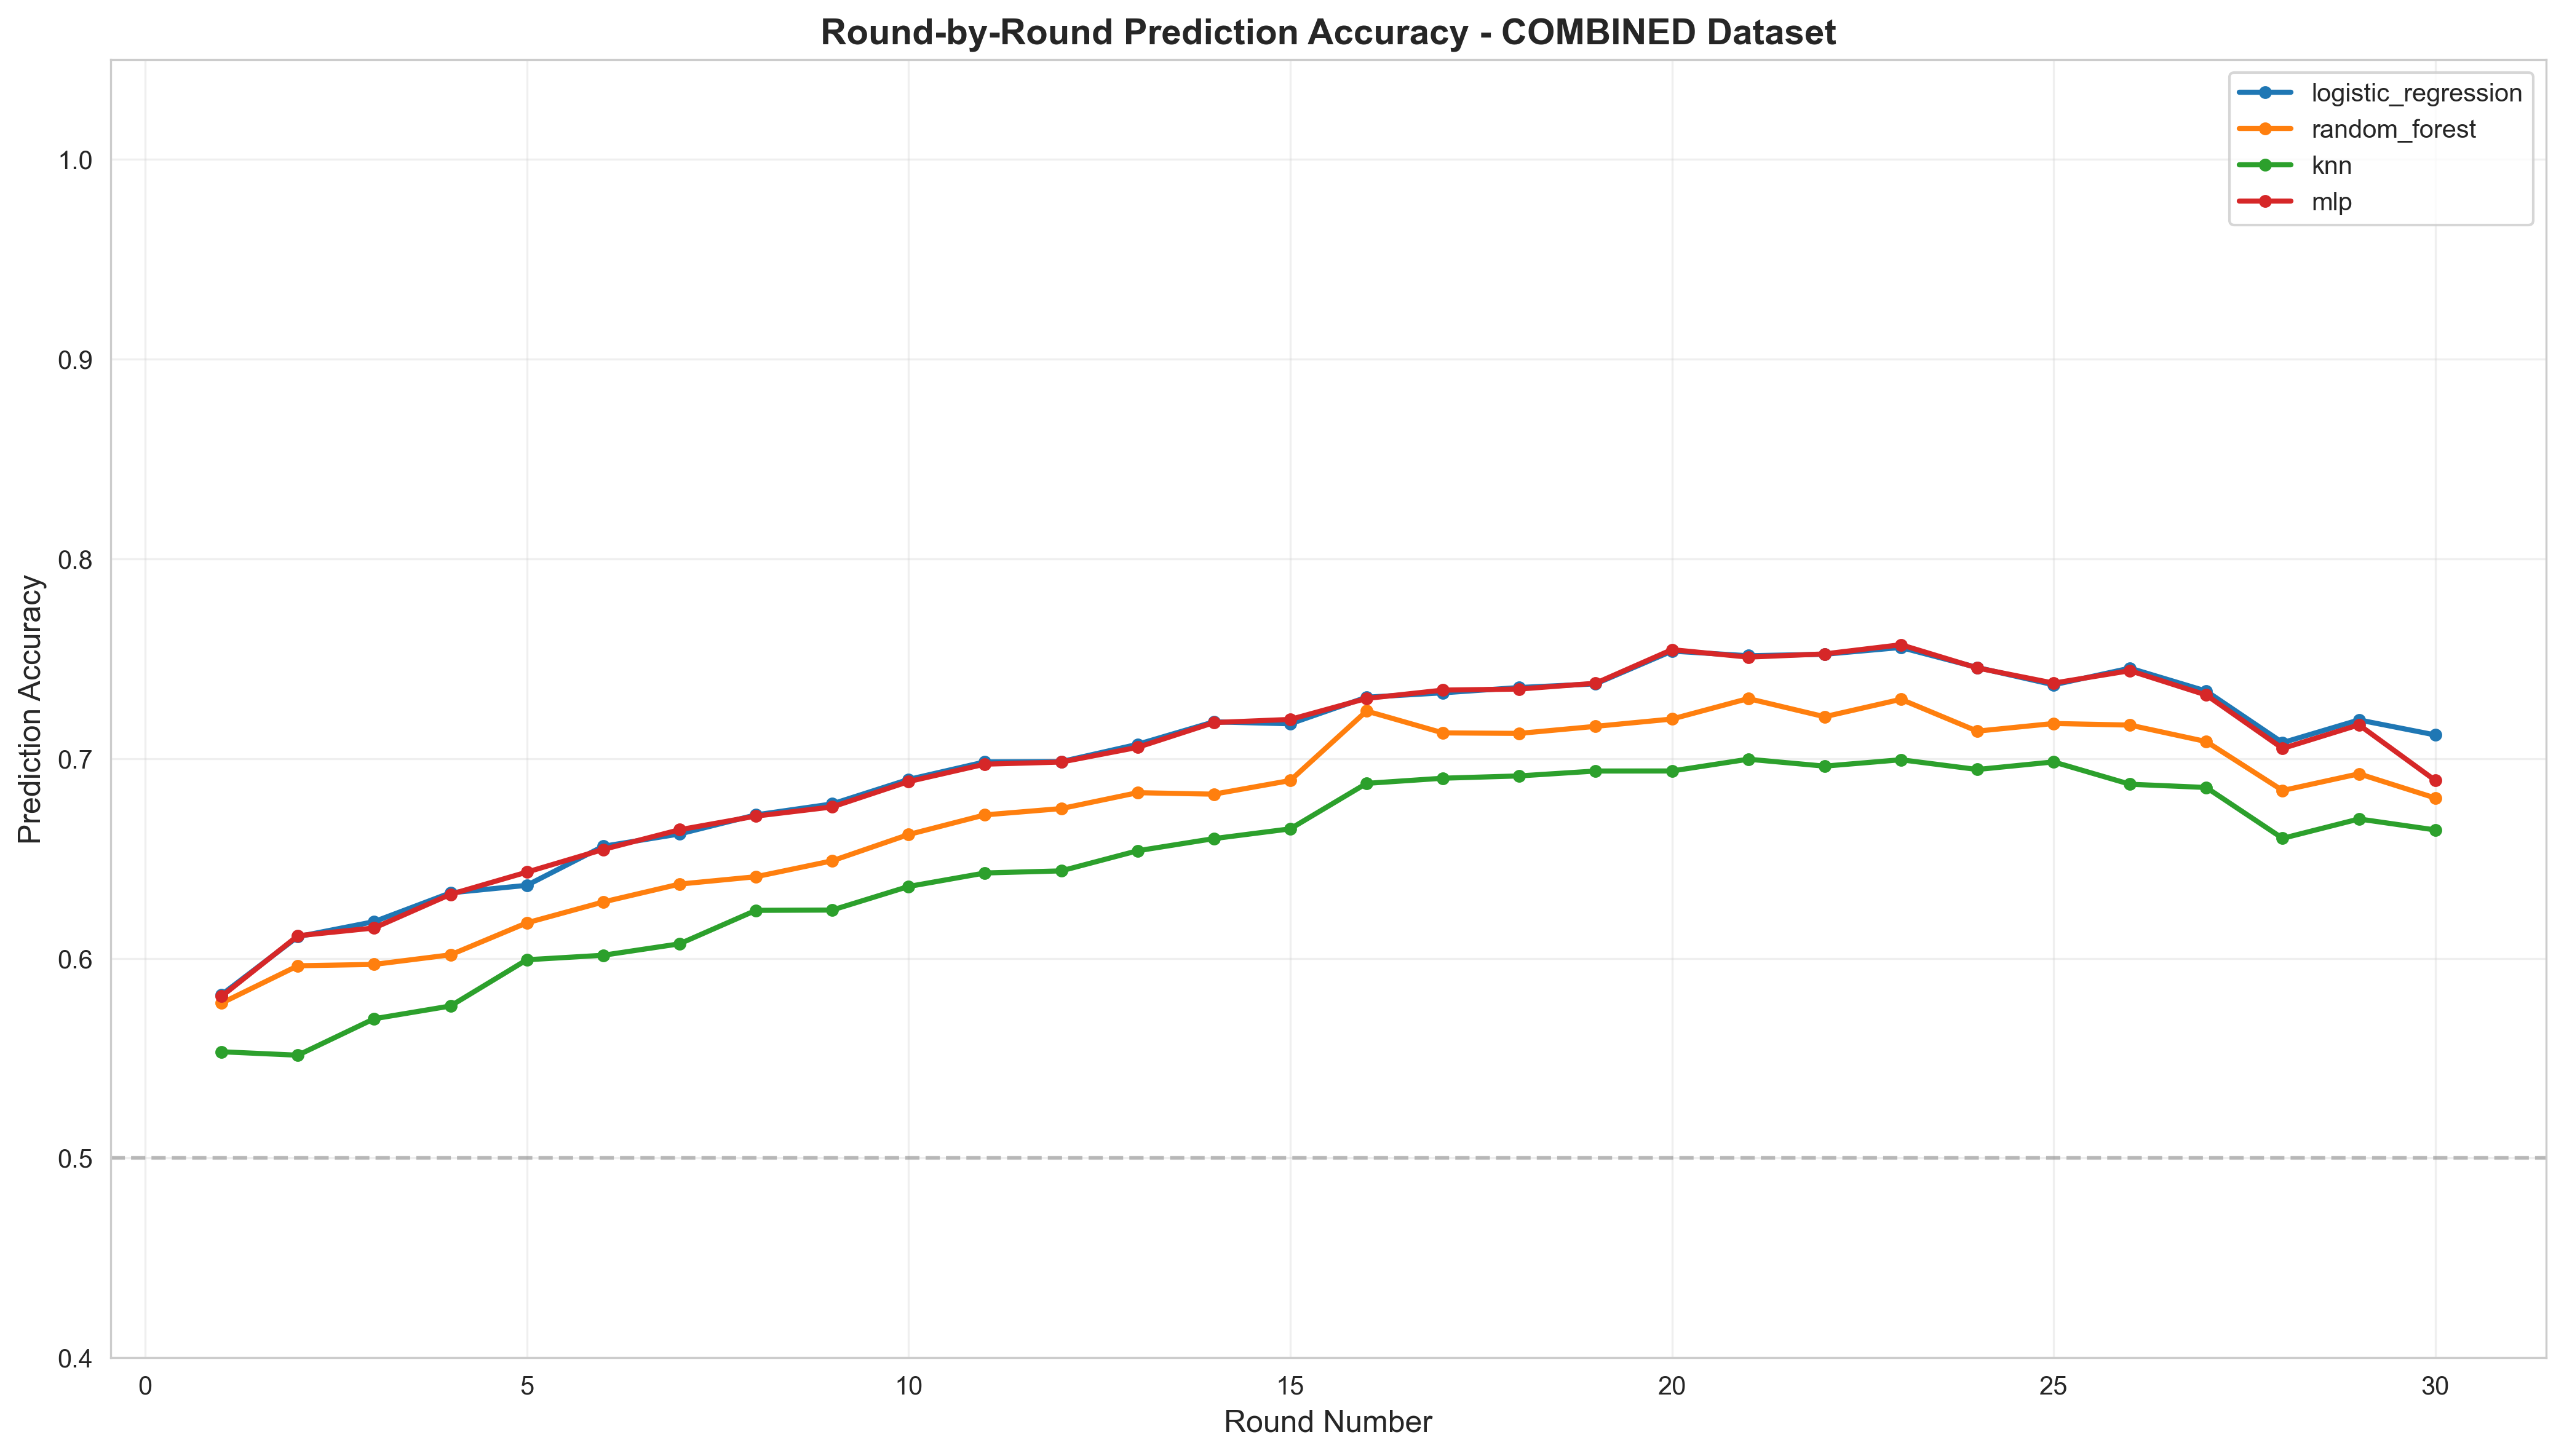
\includegraphics[width=0.9\textwidth]{results_analysis/results/round_by_round/round_by_round_accuracy_combined.png}
\caption{Round-by-round accuracy evolution across all models on the combined dataset. Accuracy improves rapidly in early rounds and plateaus around Round 15-20.}
\label{fig:round_by_round_accuracy}
\end{figure}

\begin{figure}[h]
\centering
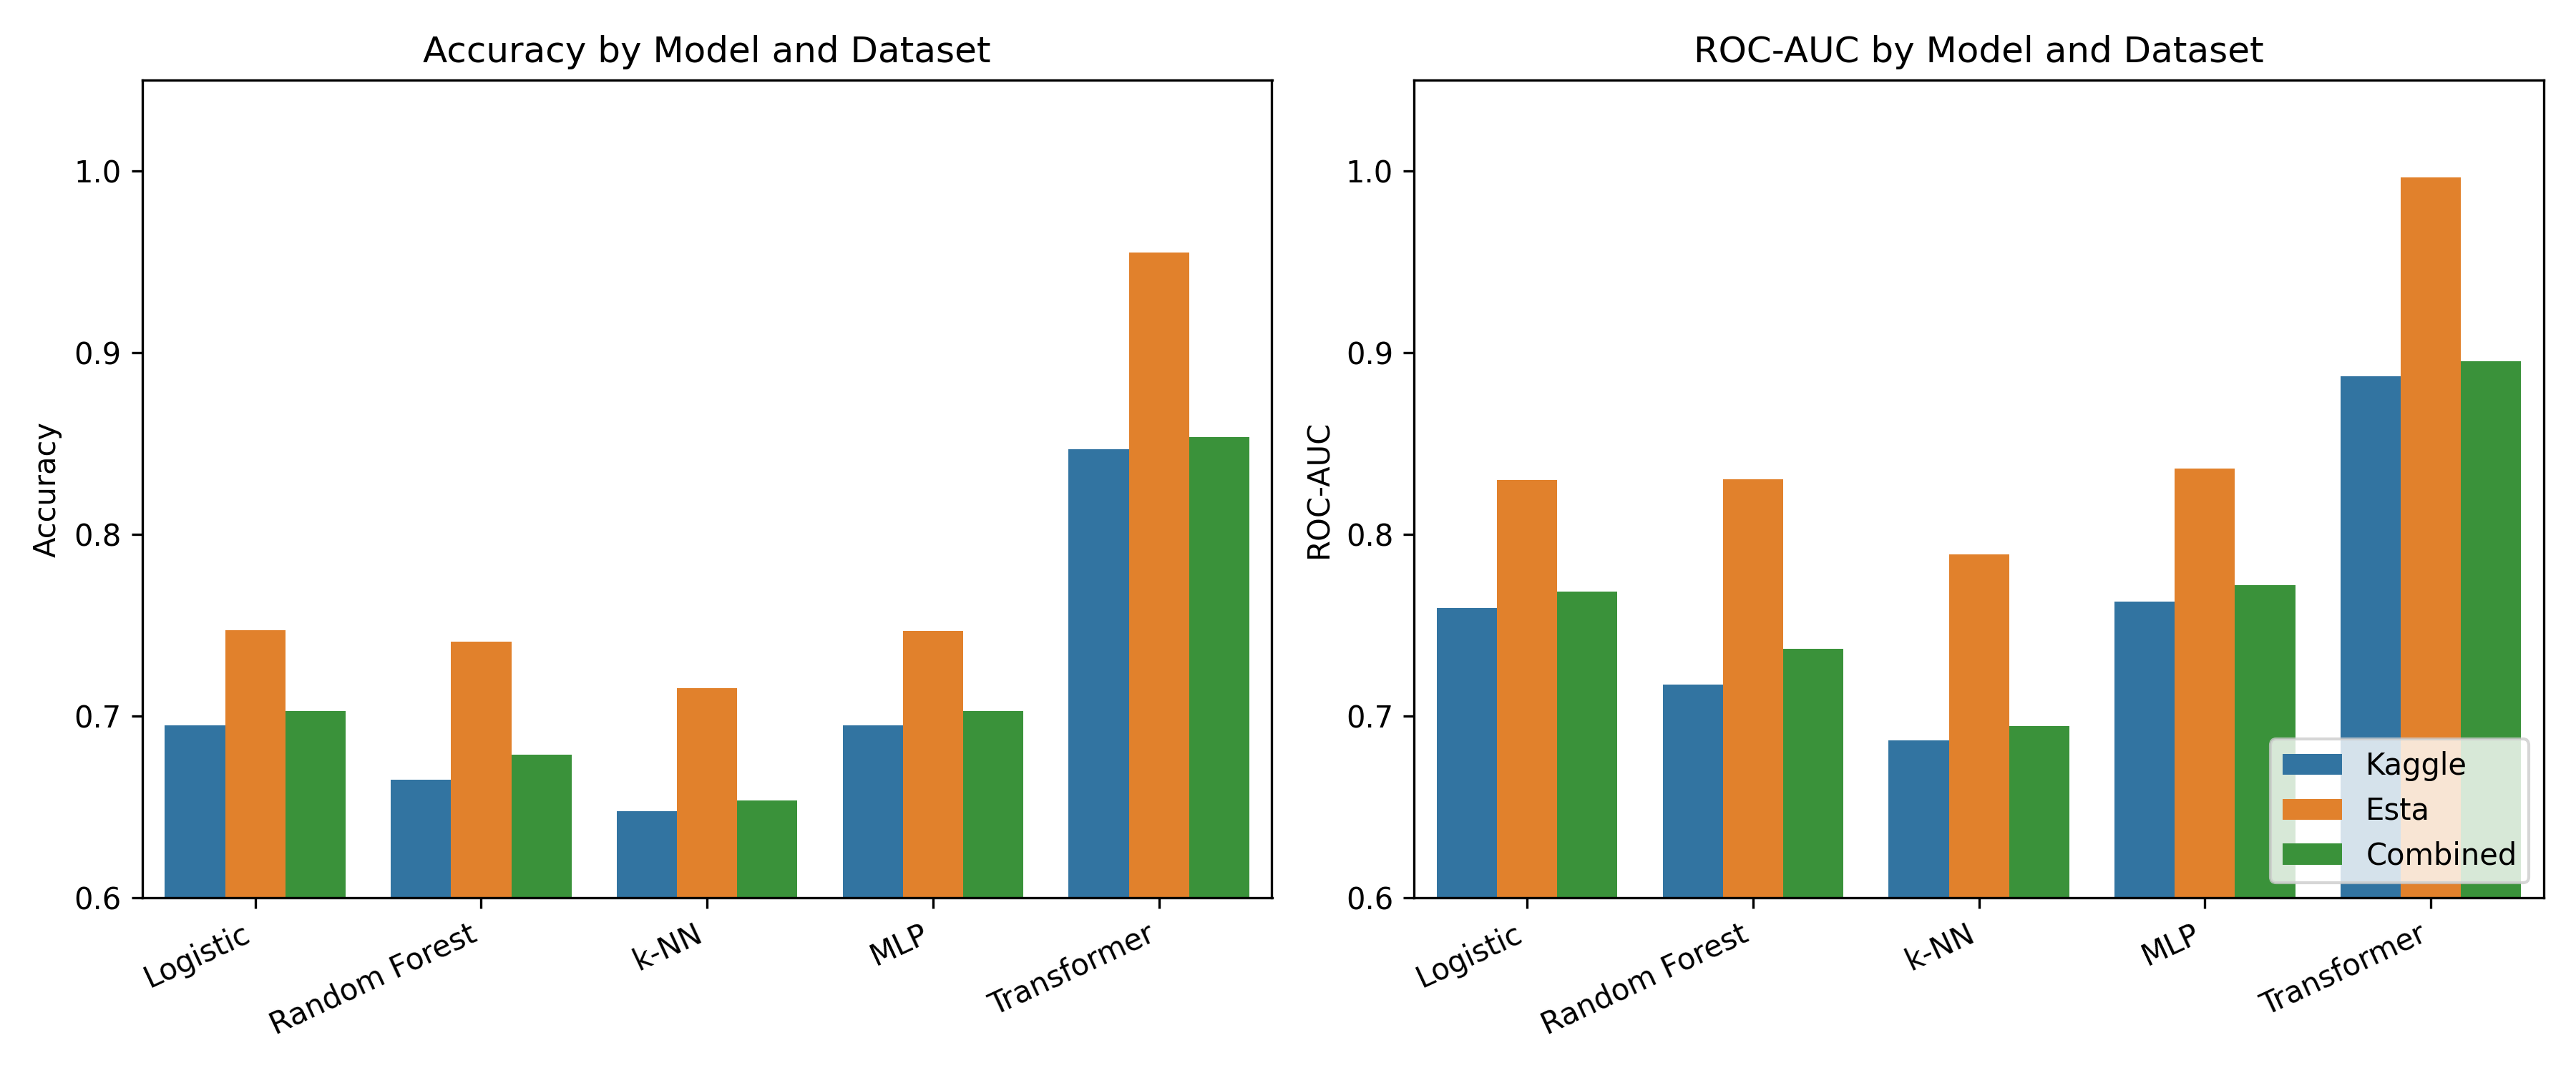
\includegraphics[width=0.9\textwidth]{results_analysis/results/figures/accuracy_roc.png}
\caption{Model accuracy and ROC-AUC comparison showing performance metrics across different models.}
\label{fig:accuracy_roc}
\end{figure}

\subsection{Calibration Analysis}

Model calibration is critical for producing reliable probability estimates. Figure~\ref{fig:calibration} shows calibration curves for all models.

\begin{figure}[h]
\centering
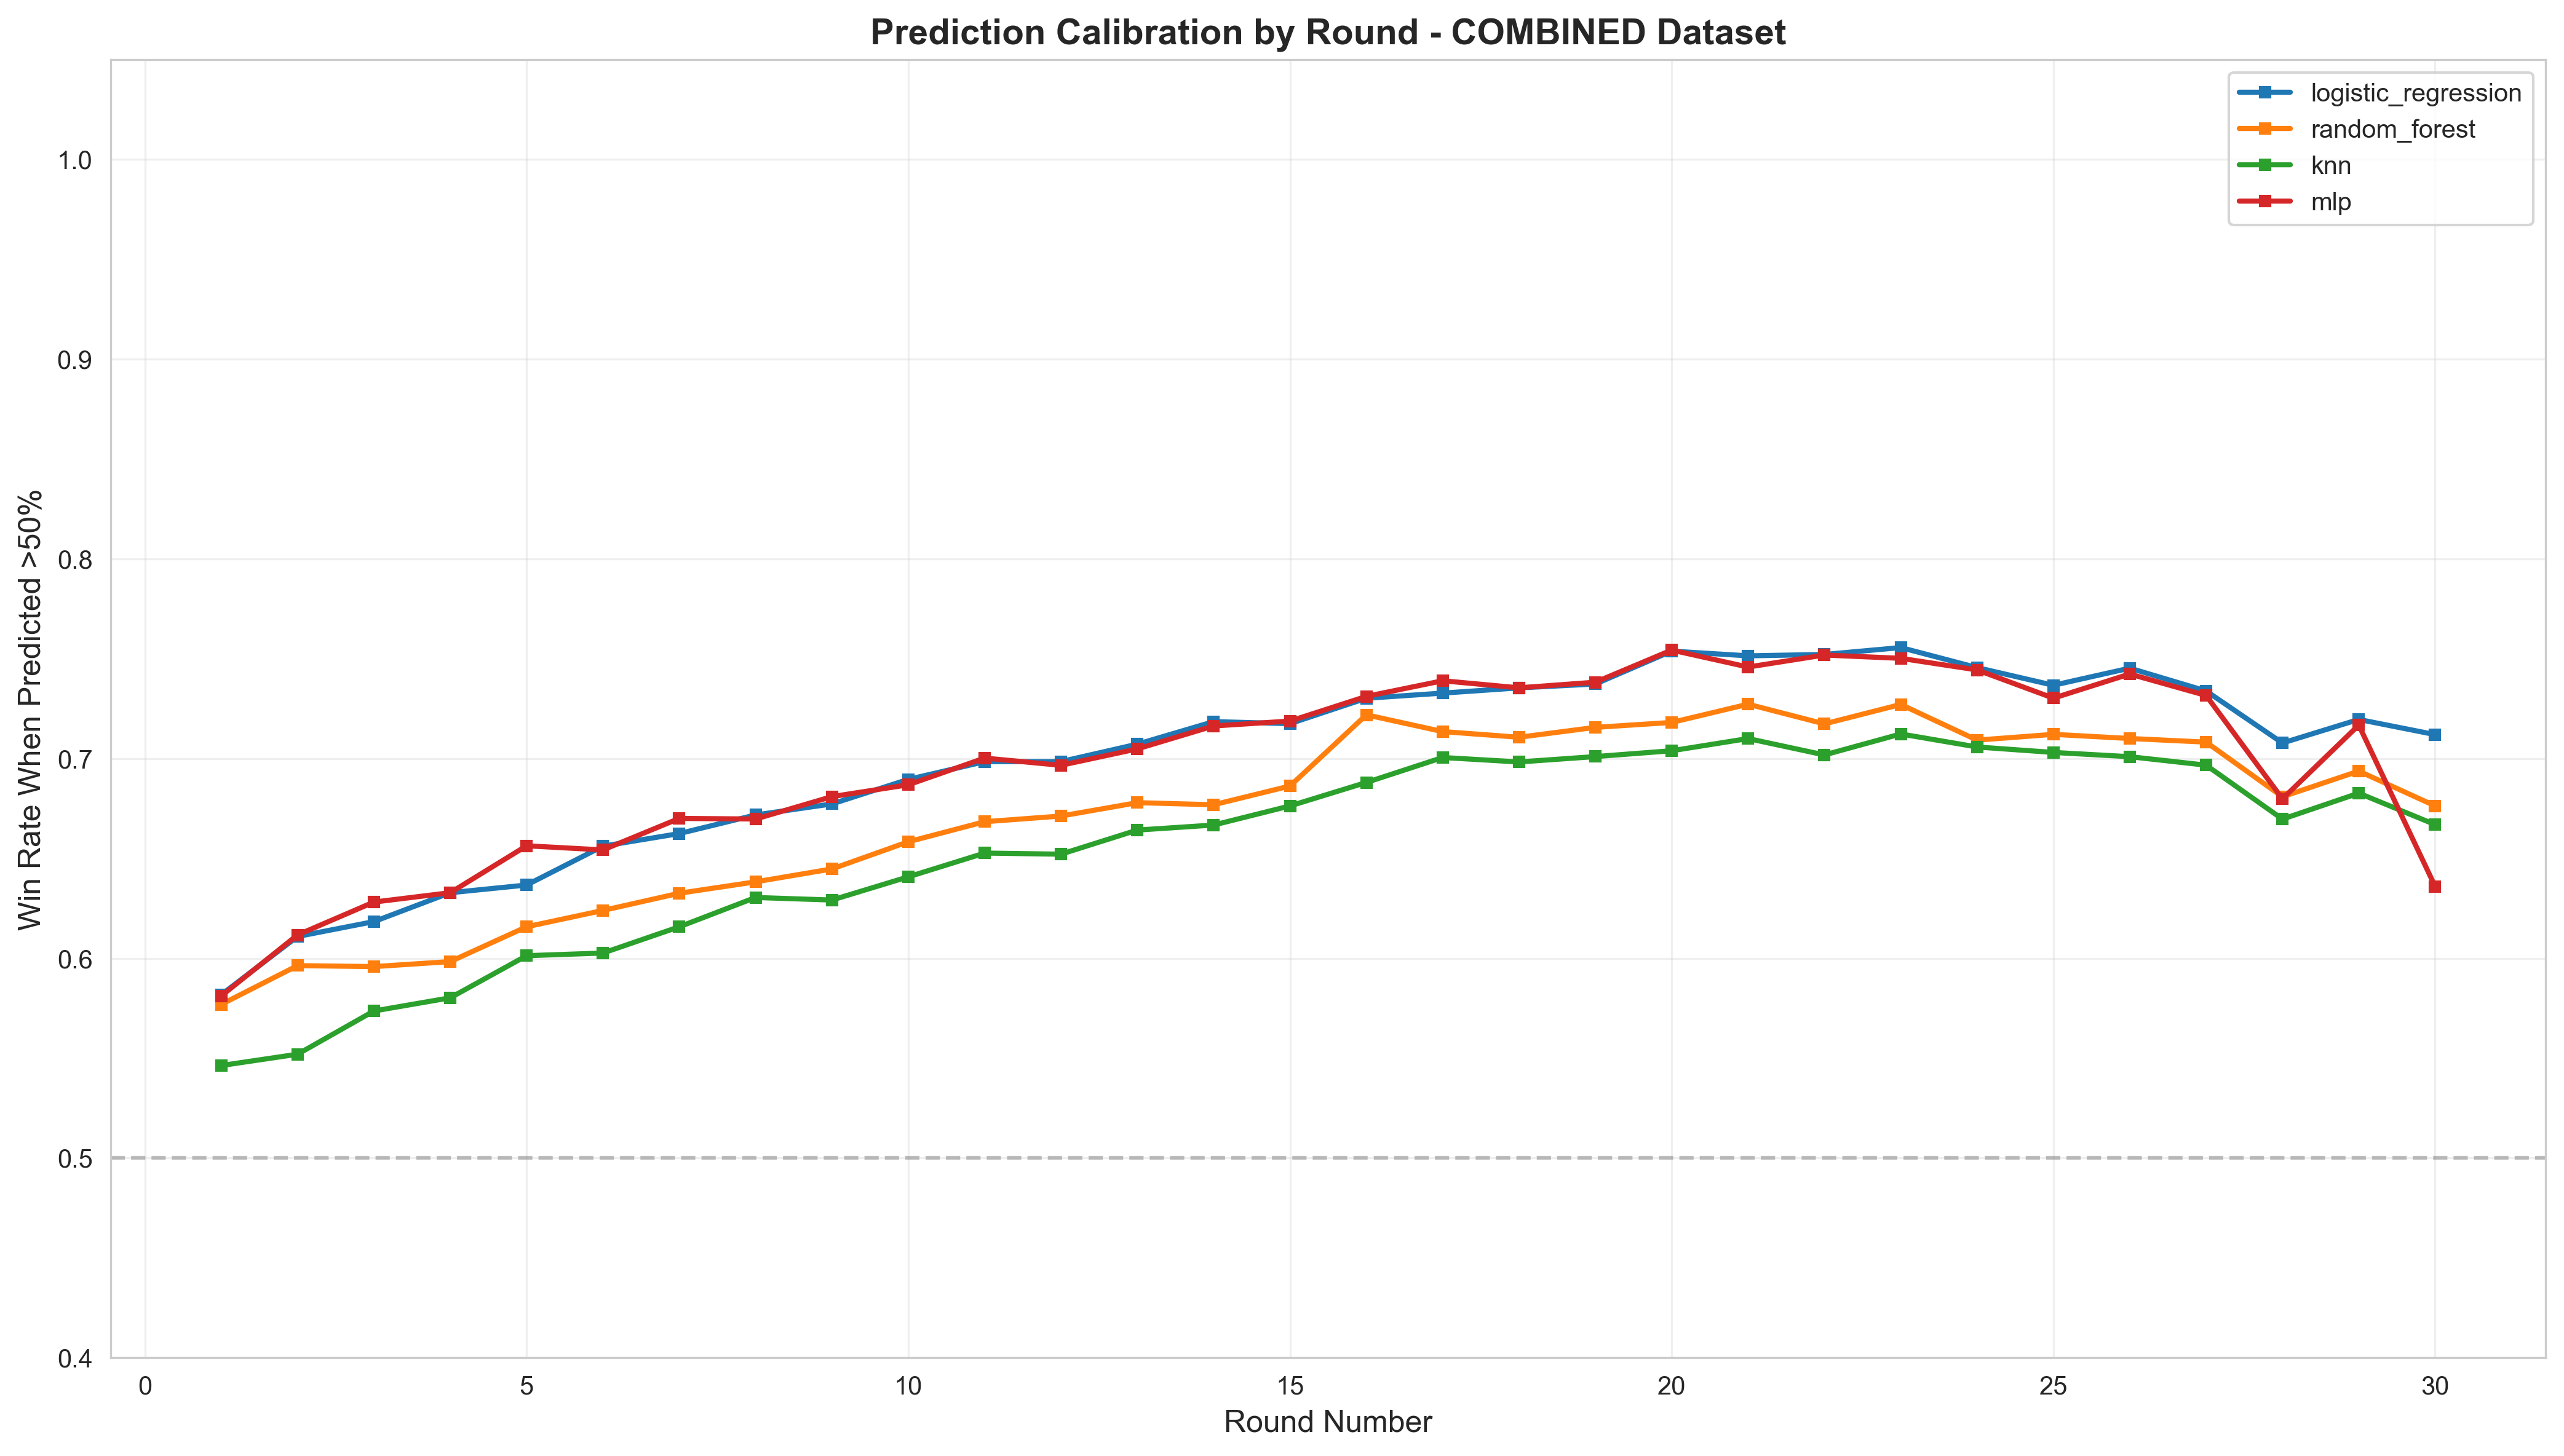
\includegraphics[width=0.9\textwidth]{results_analysis/results/round_by_round/calibration_by_round_combined.png}
\caption{Calibration analysis by round showing how well predicted probabilities match actual outcomes. Well-calibrated models follow the diagonal line.}
\label{fig:calibration}
\end{figure}

\begin{figure}[h]
\centering
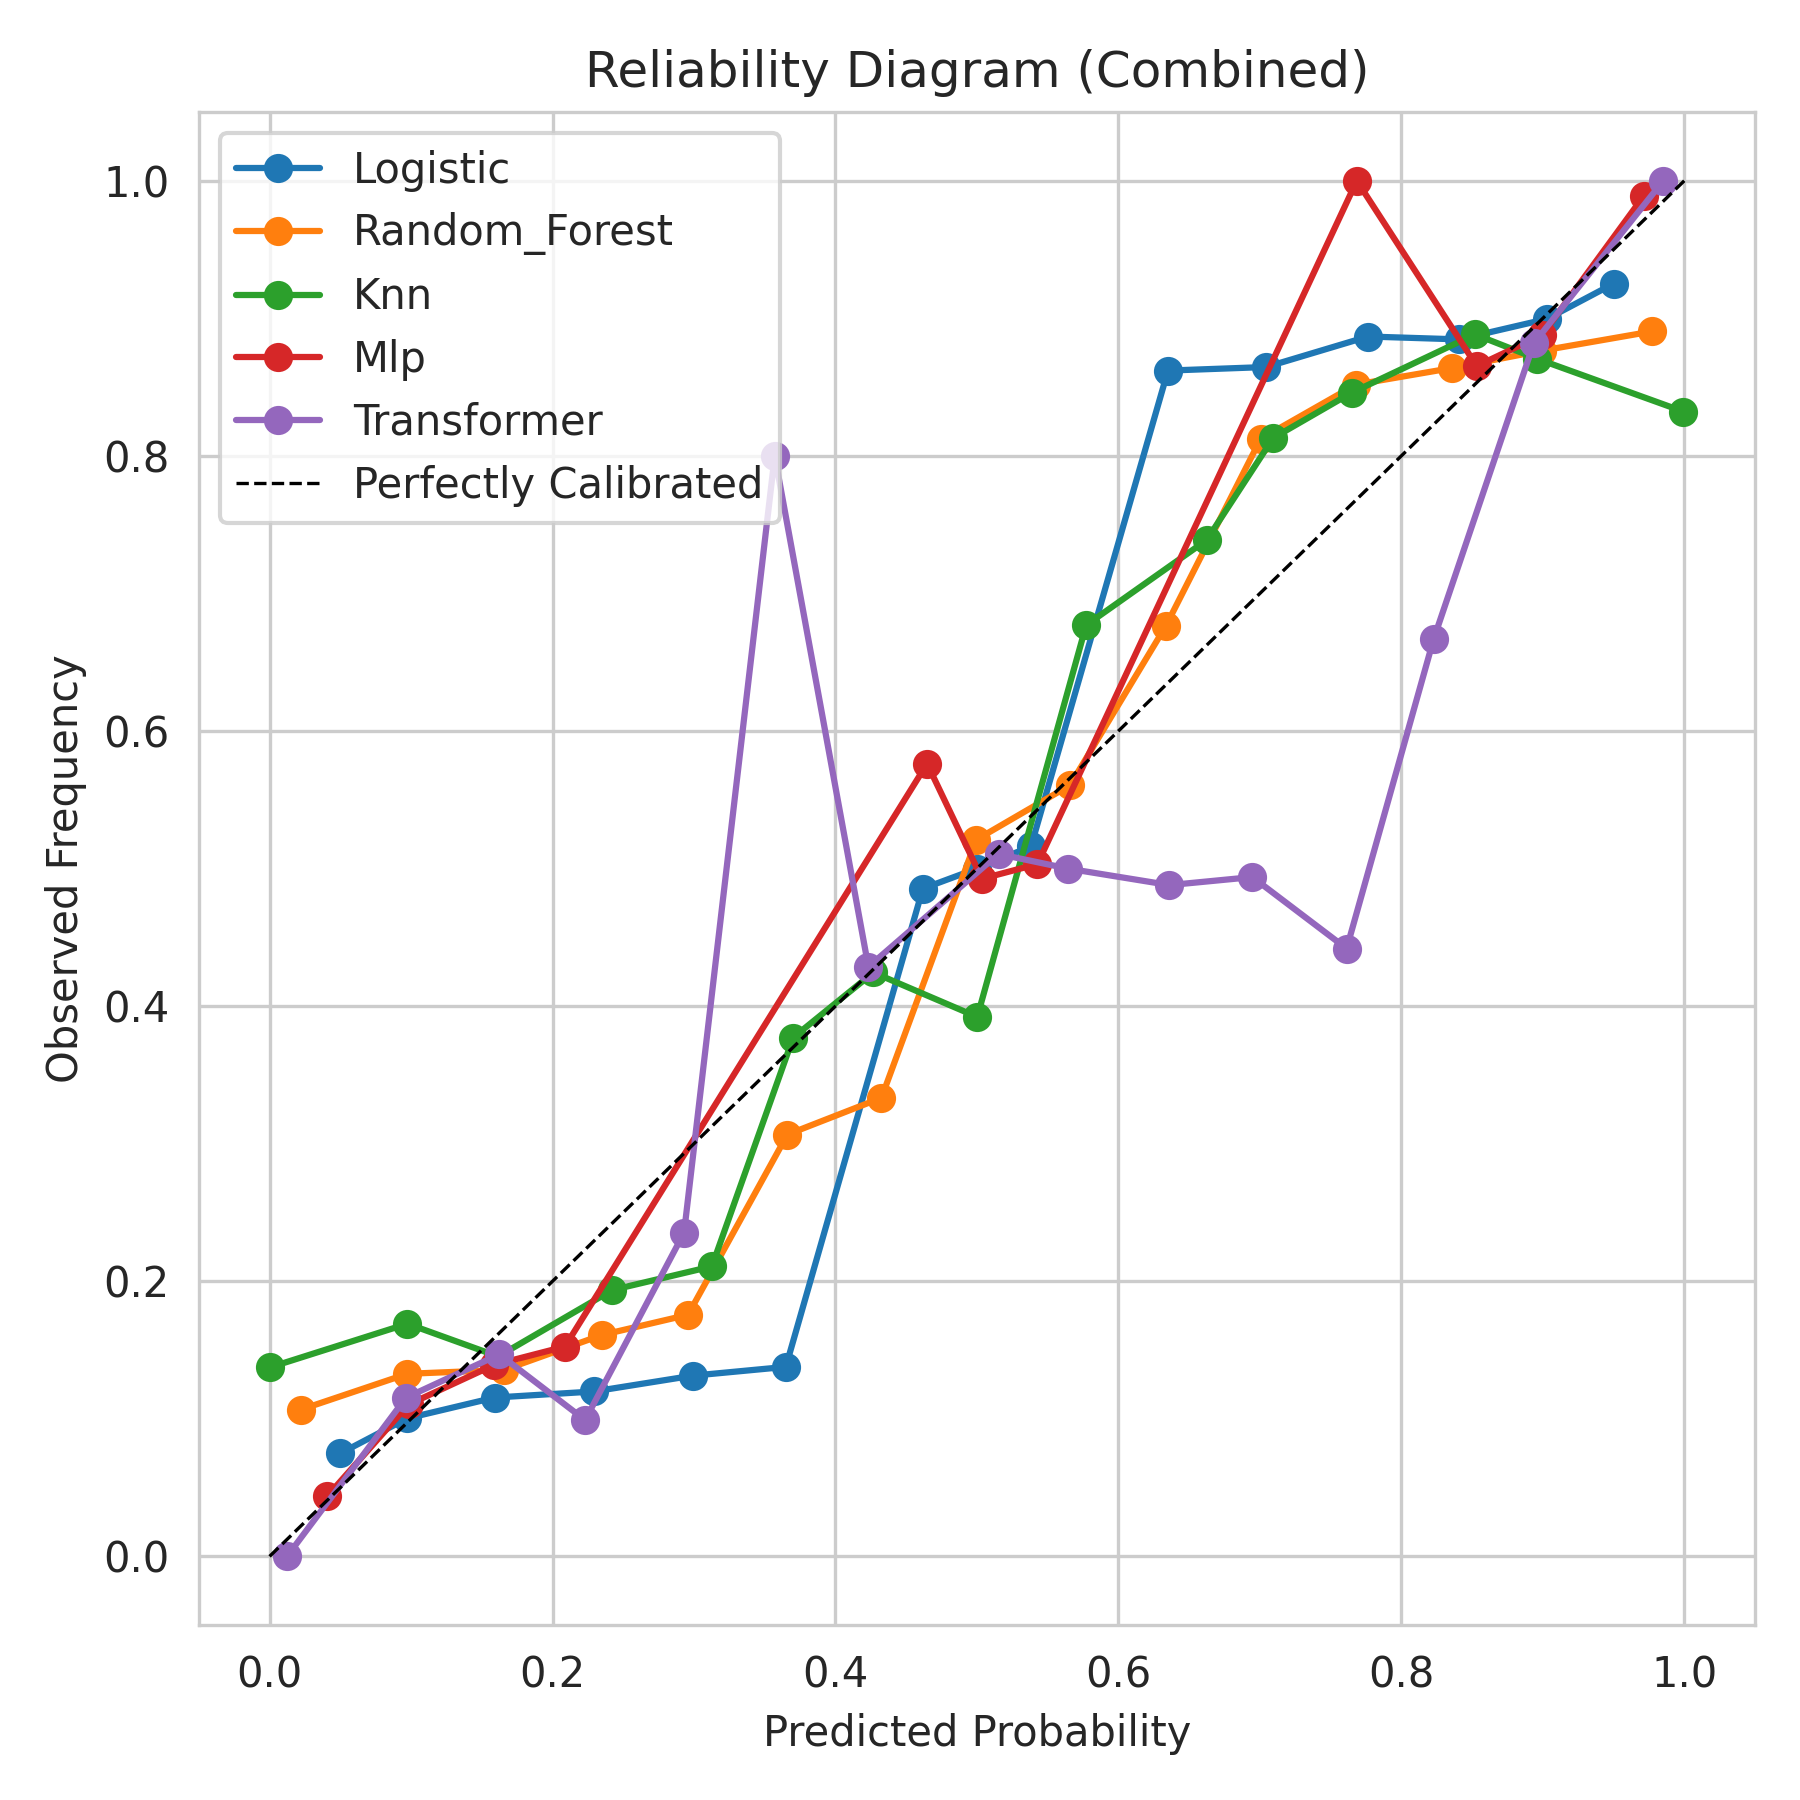
\includegraphics[width=0.9\textwidth]{results_analysis/results/figures/calibration_combined.png}
\caption{Overall calibration curves for all models across the combined dataset.}
\label{fig:calibration_overall}
\end{figure}

\subsection{Feature Importance Analysis}

Understanding which features drive predictions is essential for interpreting model decisions.

\begin{figure}[h]
\centering
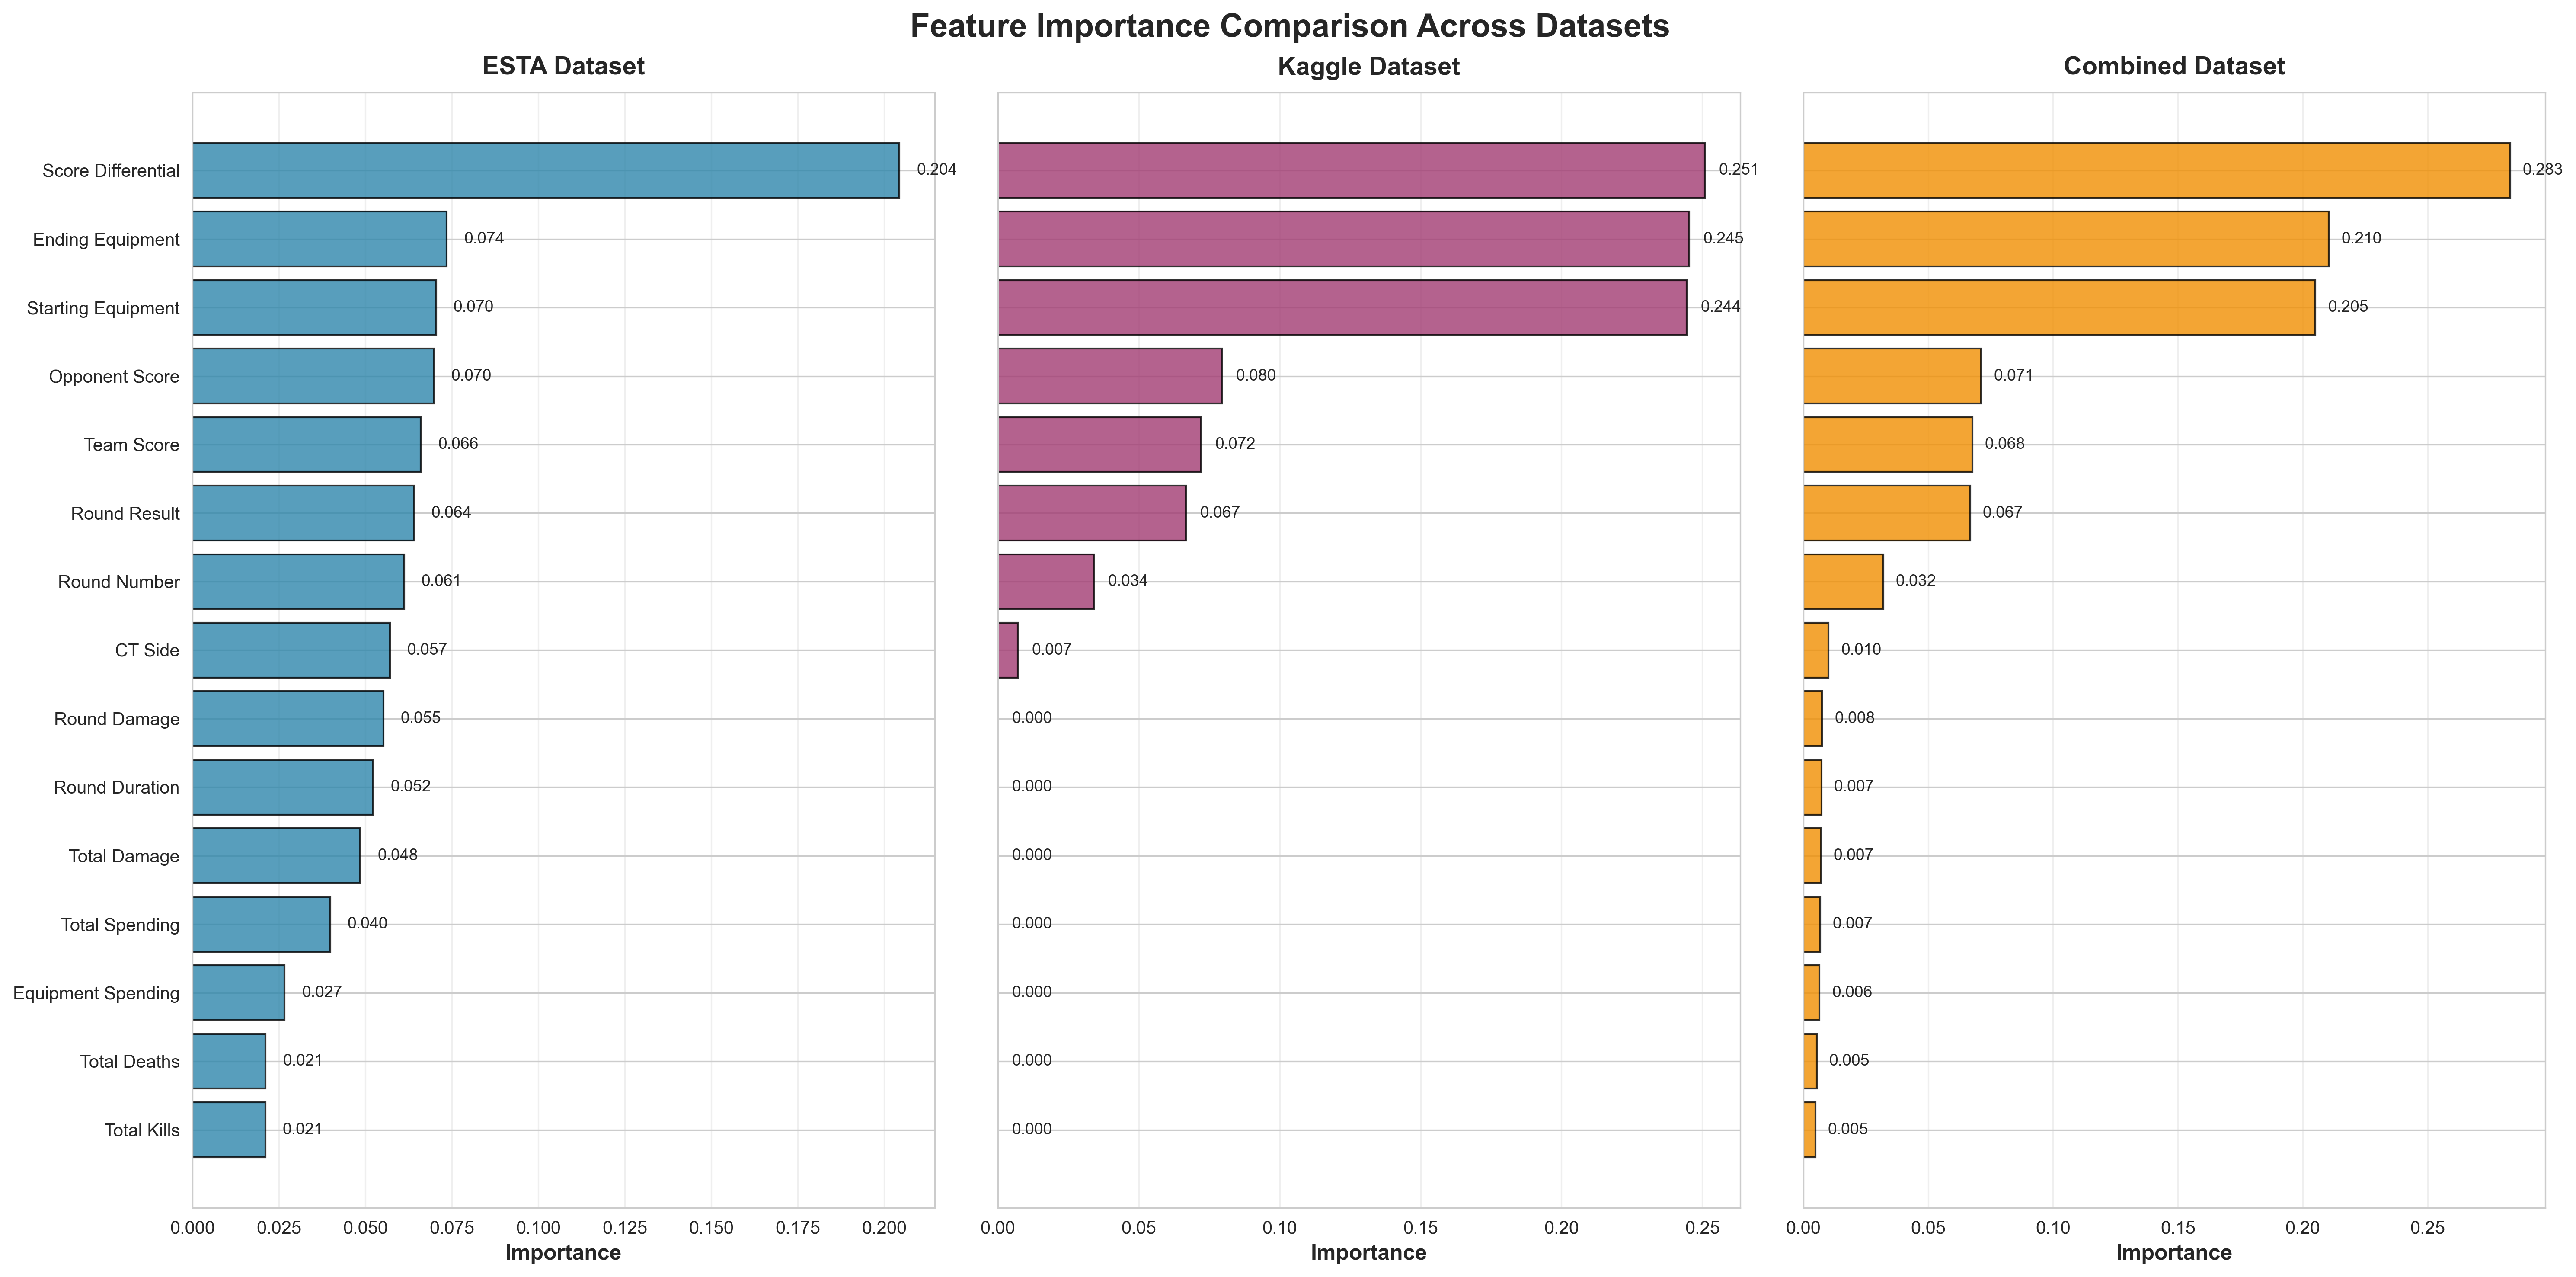
\includegraphics[width=0.9\textwidth]{results_analysis/results/feature_importance/feature_importance_comparison.png}
\caption{Feature importance comparison across different models showing the relative contribution of each feature to prediction accuracy.}
\label{fig:feature_importance}
\end{figure}

\begin{figure}[h]
\centering
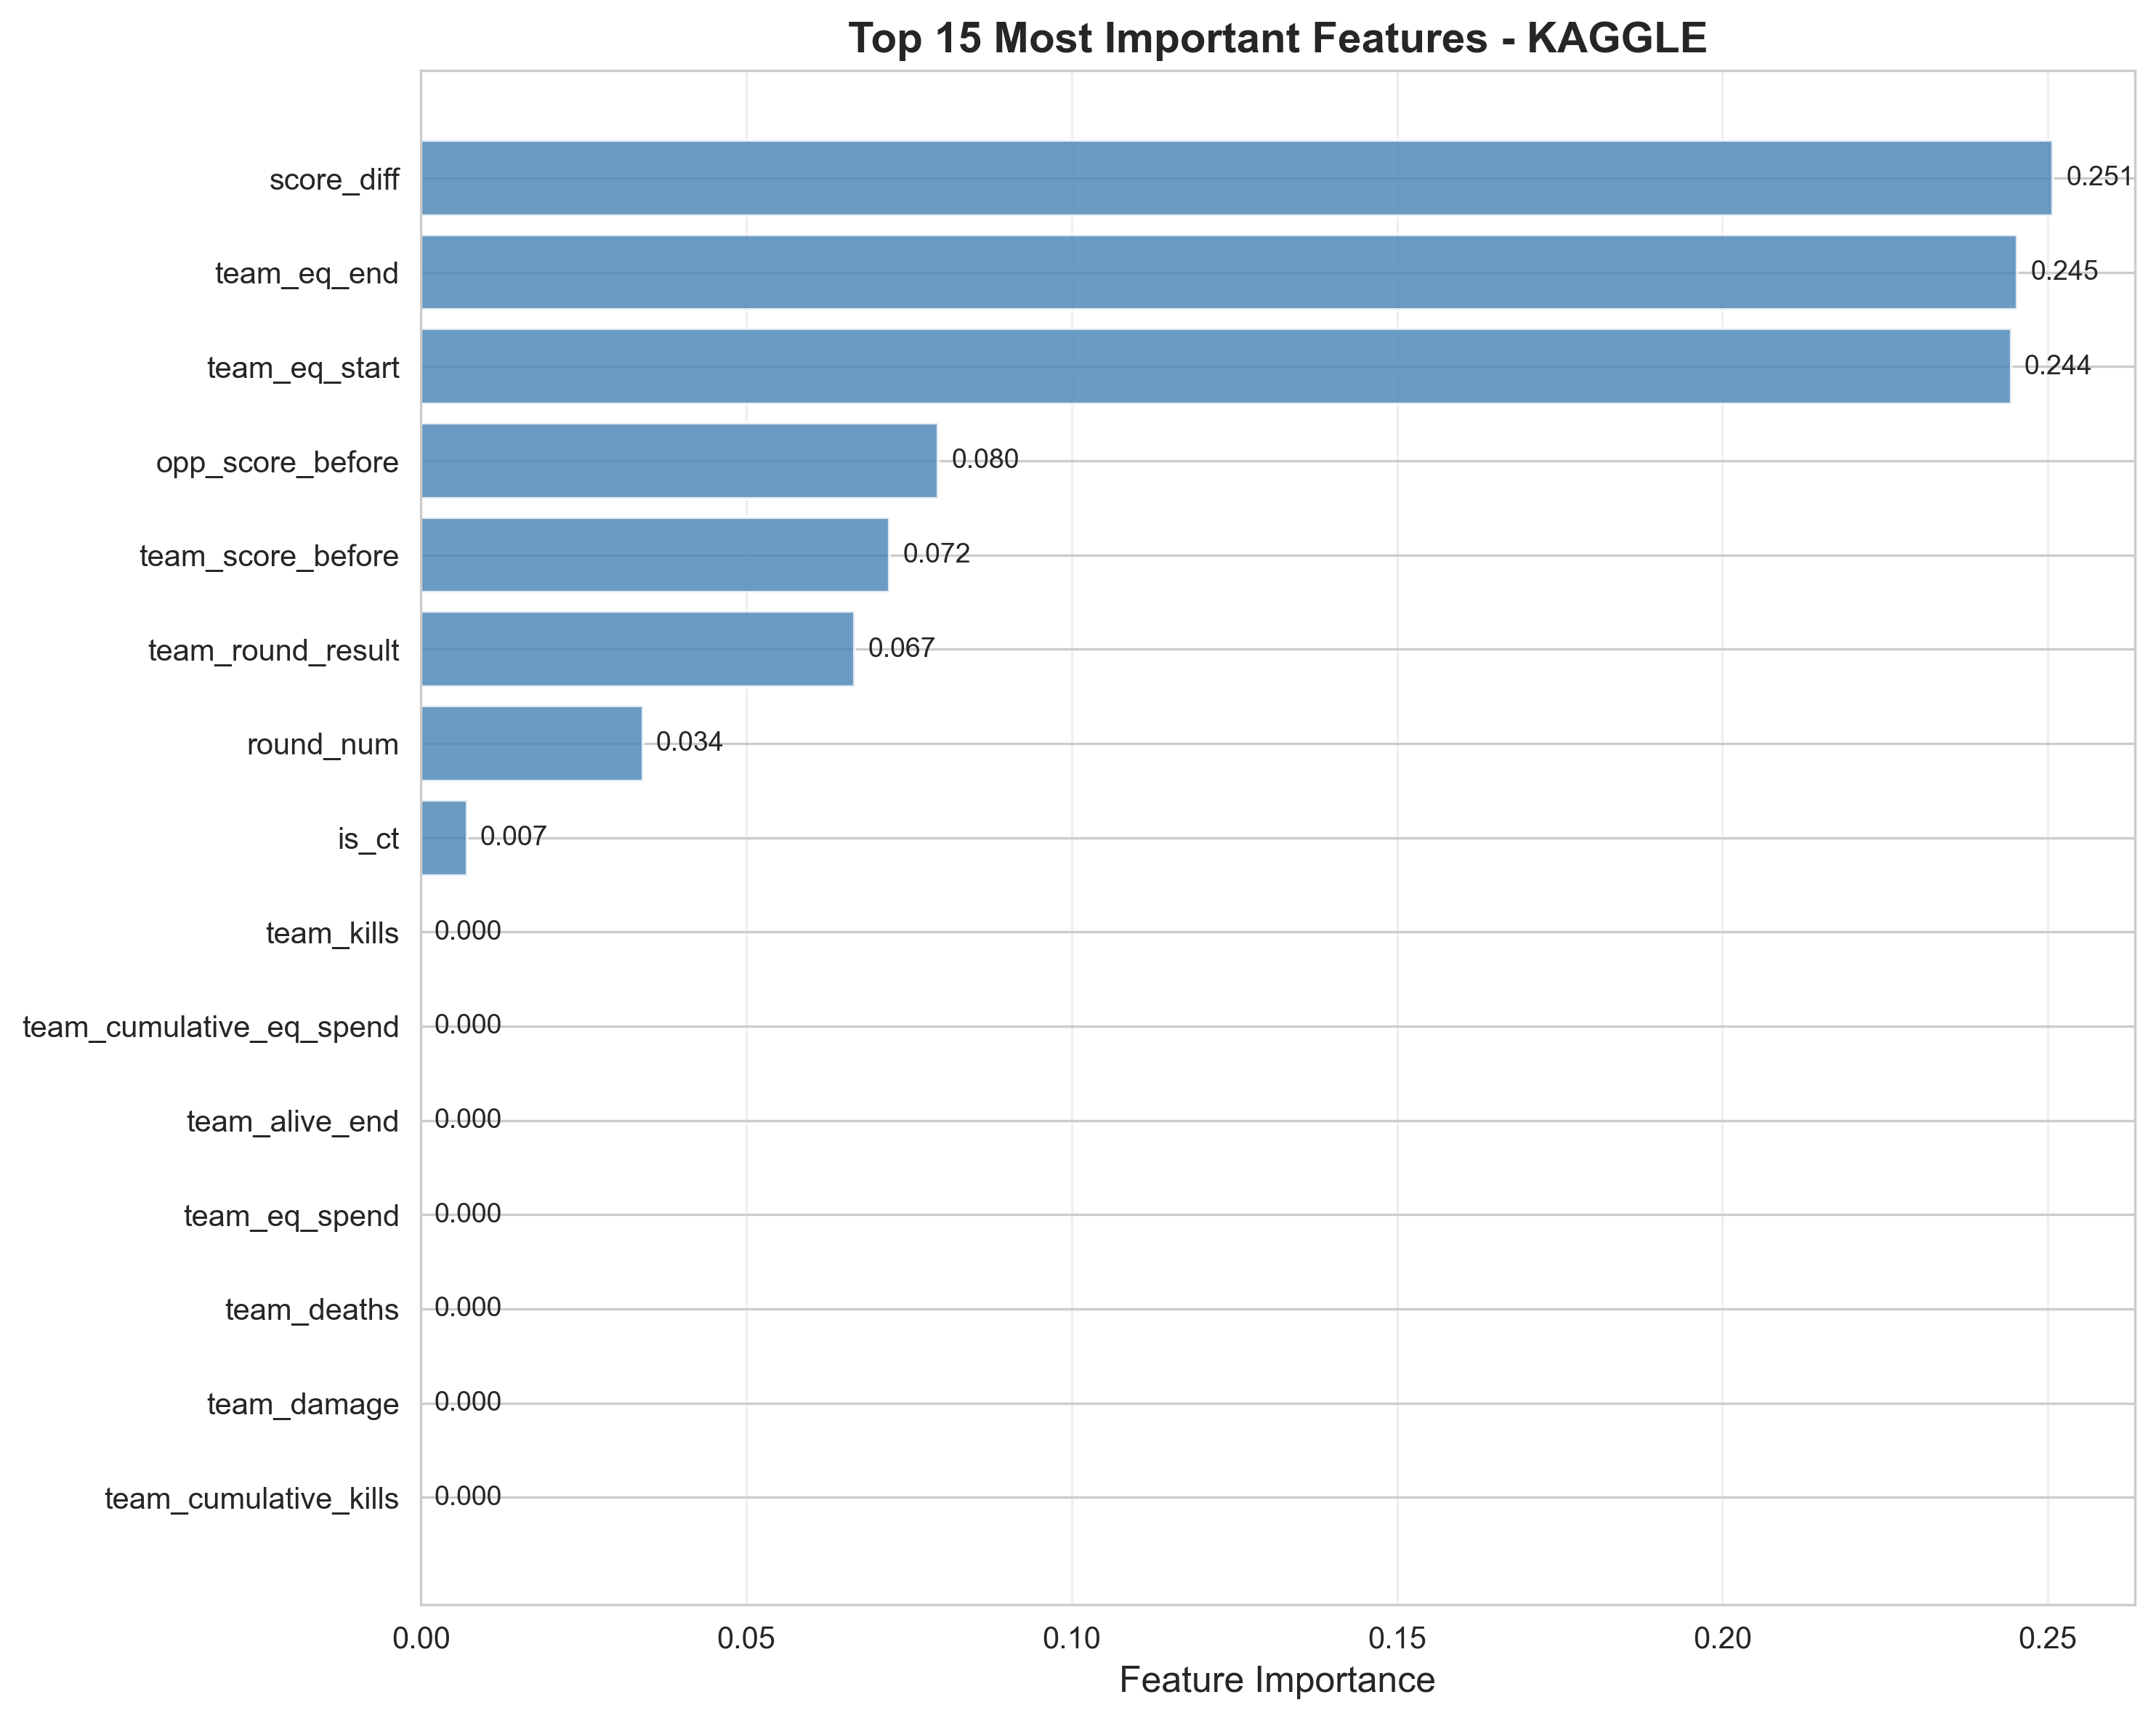
\includegraphics[width=0.9\textwidth]{results_analysis/results/extended_analysis/feature_importance_kaggle.png}
\caption{Feature importance analysis on the Kaggle dataset reveals economic features dominate predictions.}
\label{fig:feature_importance_kaggle}
\end{figure}

\subsection{Pistol Round Impact Analysis (RQ2)}

Pistol rounds---the first round of each half (rounds 1 and 16)---are considered critical due to their economic implications. Teams that win pistol rounds start the following rounds with economic advantages that can cascade through multiple rounds.

To quantify the impact of pistol rounds on match outcomes, we analyzed all matches across the three datasets, tracking which teams won rounds 1 and 16 and correlating these outcomes with final match winners. Table~\ref{tab:pistol_stats} presents the key findings.

\begin{table}[h]
\centering
\caption{Match Win Rates Based on Pistol Round Outcomes}
\label{tab:pistol_stats}
\begin{tabular}{llrrr}
\toprule
\textbf{Dataset} & \textbf{Outcome} & \textbf{Sample Size} & \textbf{Match Wins} & \textbf{Win Rate (\%)} \\
\midrule
COMBINED & Won Both Pistols & 16,793 & 10,981 & 65.4 \\
COMBINED & Won One Pistol & 32,940 & 16,470 & 50.0 \\
COMBINED & Won No Pistols & 16,791 & 5,811 & 34.6 \\
\midrule
KAGGLE & Won Both Pistols & 16,001 & 10,437 & 65.2 \\
KAGGLE & Won One Pistol & 31,418 & 15,709 & 50.0 \\
KAGGLE & Won No Pistols & 16,000 & 5,563 & 34.8 \\
\midrule
ESTA & Won Both Pistols & 792 & 544 & 68.7 \\
ESTA & Won One Pistol & 1,522 & 761 & 50.0 \\
ESTA & Won No Pistols & 791 & 248 & 31.4 \\
\bottomrule
\end{tabular}
\end{table}

\textbf{Key Findings:}
\begin{itemize}
    \item \textbf{Both Pistols Won:} Teams winning both pistol rounds (R1 and R16) achieve 65-69\% match win rates across all datasets, representing a substantial advantage.
    \item \textbf{Split Pistols:} Teams winning exactly one pistol round have approximately 50\% win rates, indicating that pistol round wins roughly balance out when split between teams.
    \item \textbf{No Pistols Won:} Teams losing both pistol rounds face severe disadvantages, winning only 31-35\% of matches.
    \item \textbf{30-35 Percentage Point Swing:} The difference between winning both pistols (65-69\%) versus winning neither (31-35\%) represents a 30-38 percentage point swing in match win probability.
    \item \textbf{Individual Pistol Impact:} Both Round 1 and Round 16 pistol wins correlate with approximately 58\% match win rates, showing similar importance for both halves.
    \item \textbf{Consistency Across Datasets:} The pistol round effect is remarkably consistent across ESTA, Kaggle, and Combined datasets, validating the robustness of this finding.
\end{itemize}

\begin{figure}[h]
\centering
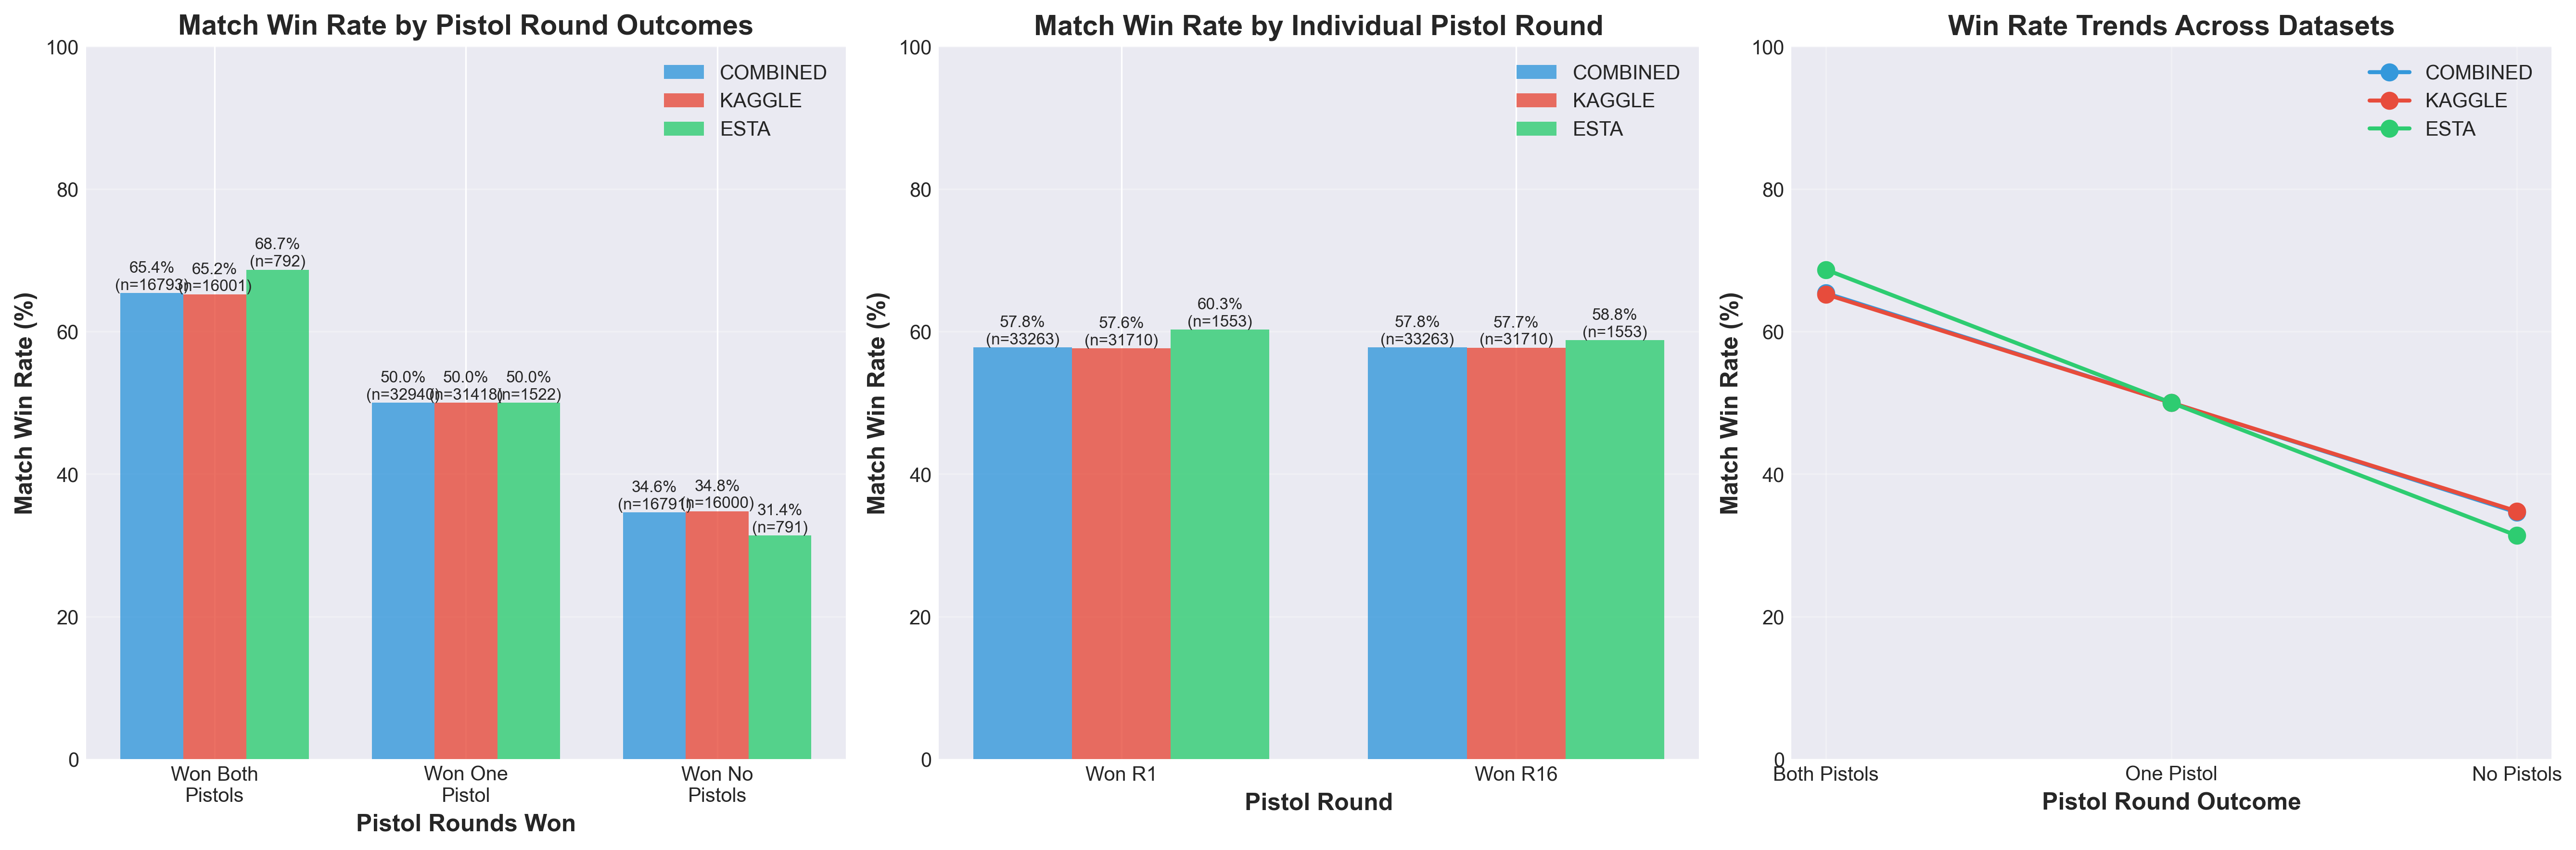
\includegraphics[width=0.95\textwidth]{results_analysis/results/pistol_analysis/pistol_round_win_rates.png}
\caption{Match win rates based on pistol round outcomes across all three datasets. Teams winning both pistol rounds achieve 65-69\% match win rates, while teams losing both pistols win only 31-35\% of matches. The 30+ percentage point difference demonstrates the critical importance of pistol round performance.}
\label{fig:pistol_analysis}
\end{figure}

\textbf{Strategic Implications:}

The pistol round analysis provides empirical evidence for several strategic insights:

\begin{enumerate}
    \item \textbf{Economic Cascades:} Winning pistol rounds provides immediate economic advantages (equipment savings) that enable stronger purchases in subsequent rounds, creating a positive feedback loop.
    \item \textbf{Momentum Building:} The 15+ percentage point advantage from winning one additional pistol (from 50\% to 65\%) suggests that early-game momentum significantly impacts match outcomes.
    \item \textbf{Comeback Difficulty:} Teams losing both pistols face uphill battles, winning fewer than one-third of matches, emphasizing the importance of pistol round preparation and execution.
    \item \textbf{Practice Focus:} The substantial impact of pistol rounds (30-38pp swing) justifies significant practice time dedicated to pistol-only scenarios in competitive training regimens.
\end{enumerate}

\subsection{Transformer Model Performance}

The Transformer Encoder model significantly outperforms all traditional machine learning approaches, demonstrating the value of sequential modeling for match prediction.

\begin{table}[h]
\centering
\caption{Transformer Model Performance Across Datasets}
\begin{tabular}{lcccc}
\toprule
\textbf{Dataset} & \textbf{Accuracy} & \textbf{Log Loss} & \textbf{Brier Score} & \textbf{ROC-AUC} \\
\midrule
ESTA & 97.8\% & 0.044 & 0.013 & 0.999 \\
Kaggle & 84.7\% & 0.395 & 0.118 & 0.887 \\
Combined & 84.6\% & 0.395 & 0.118 & 0.890 \\
\bottomrule
\end{tabular}
\end{table}

\subsection{ROC Curves and Classification Metrics}

Receiver Operating Characteristic (ROC) curves provide insight into model discrimination ability across different probability thresholds.

\begin{figure}[h]
\centering
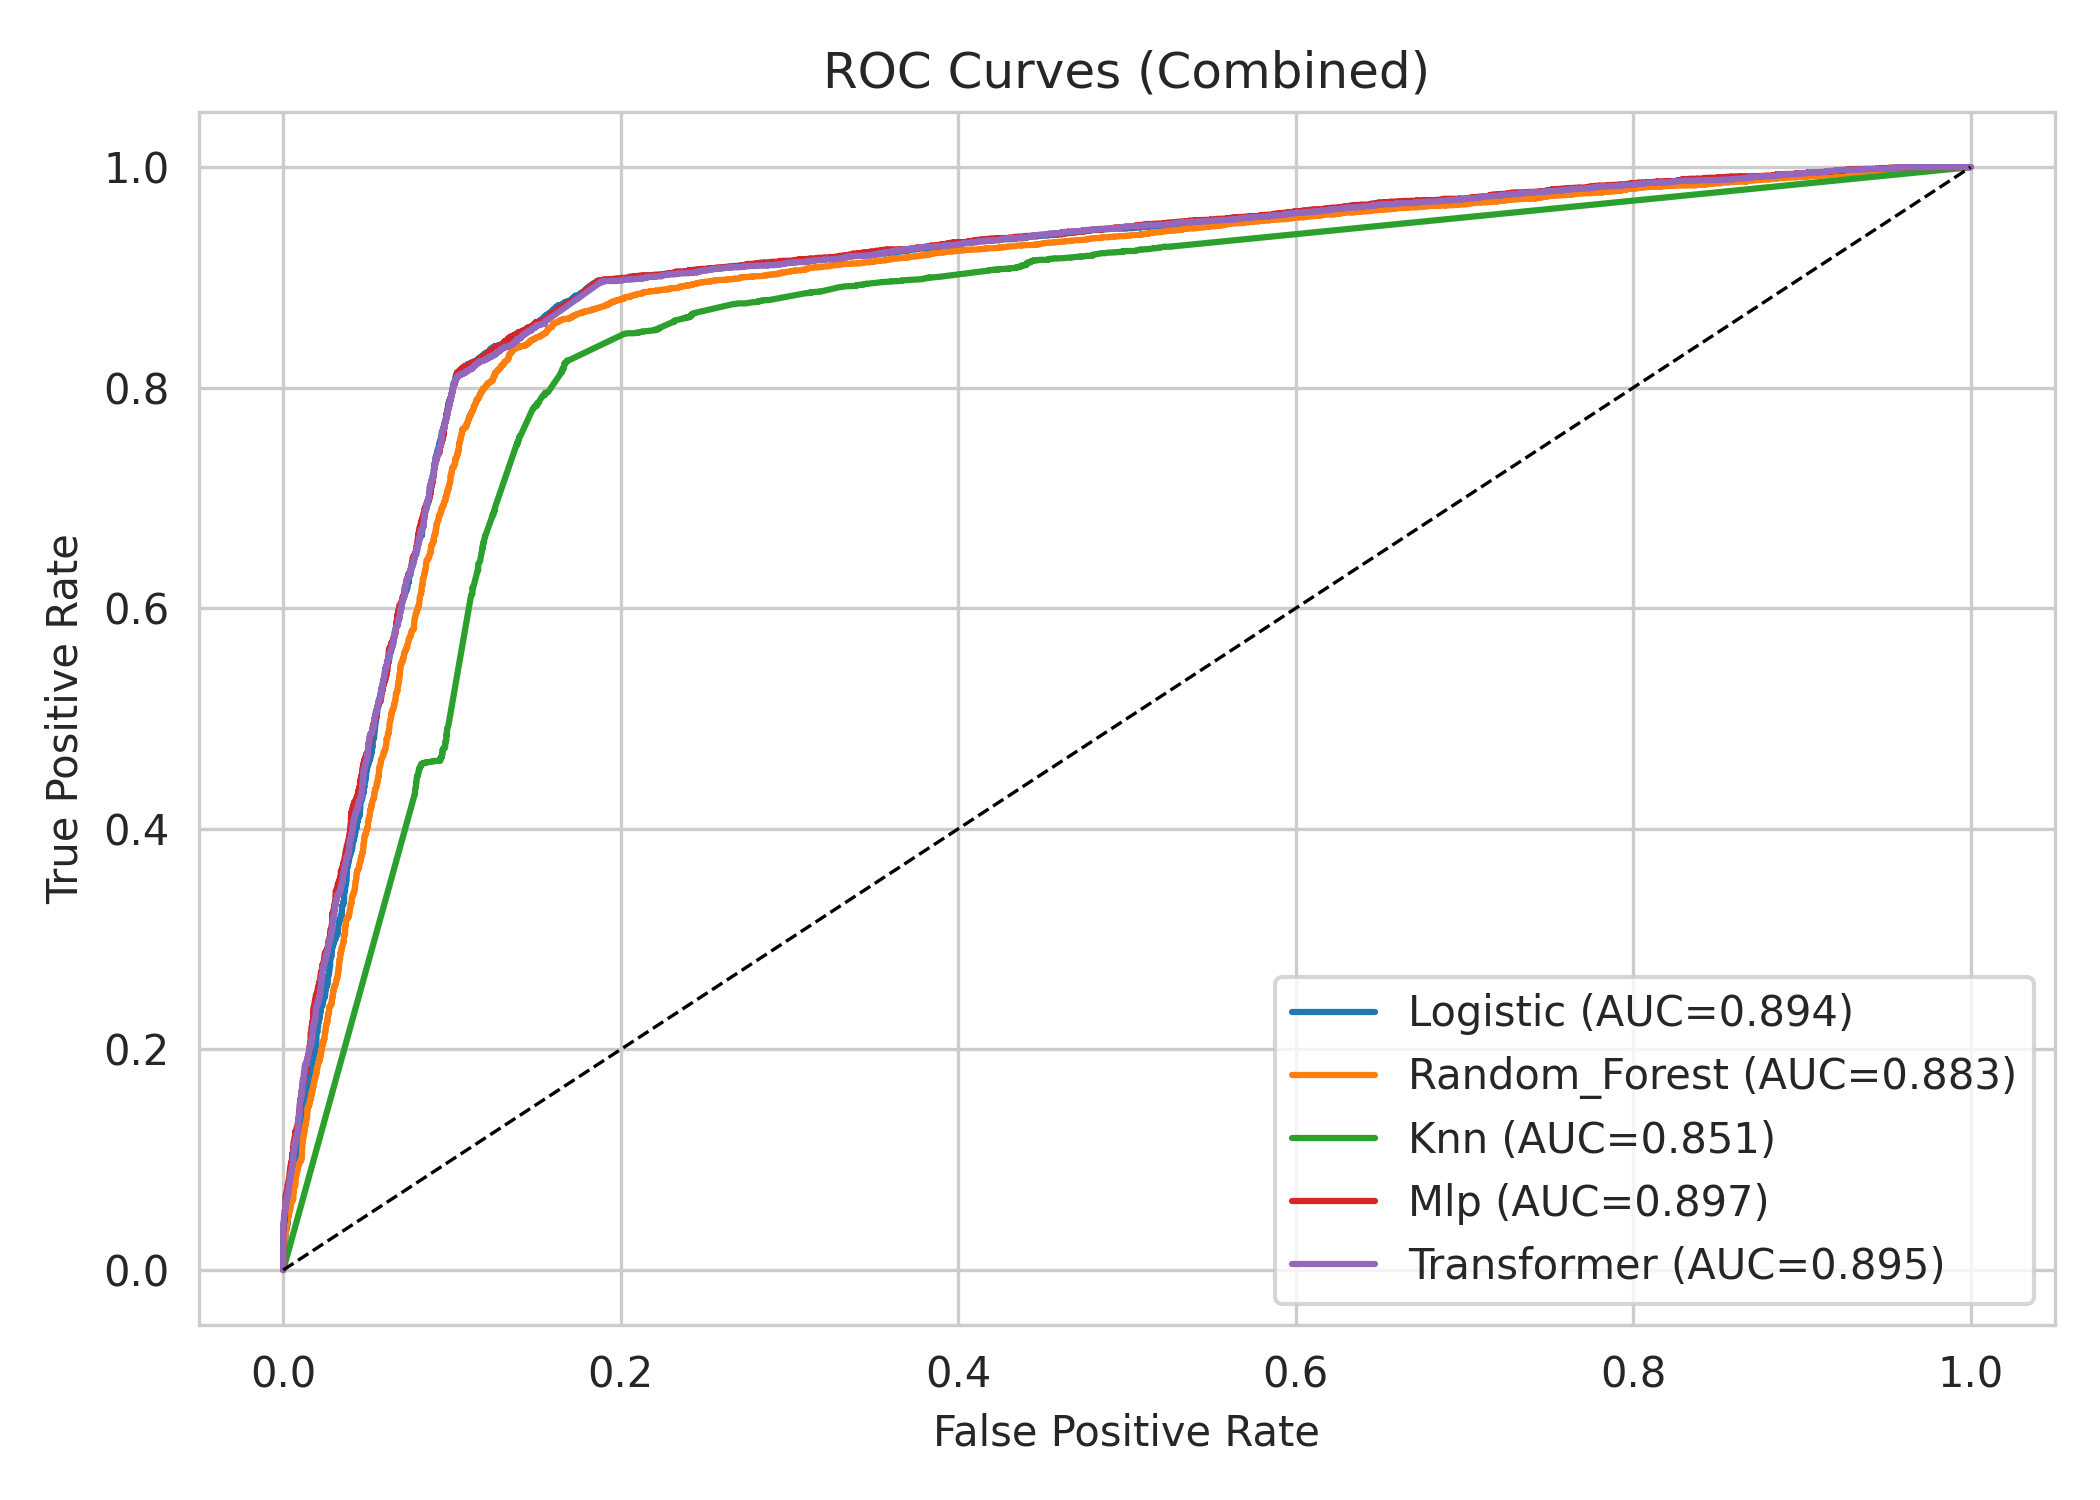
\includegraphics[width=0.9\textwidth]{results_analysis/results/figures/roc_curves_combined.png}
\caption{ROC curves for all models on the combined dataset. Higher AUC values indicate better discrimination between match winners and losers.}
\label{fig:roc_curves}
\end{figure}

\begin{figure}[h]
\centering
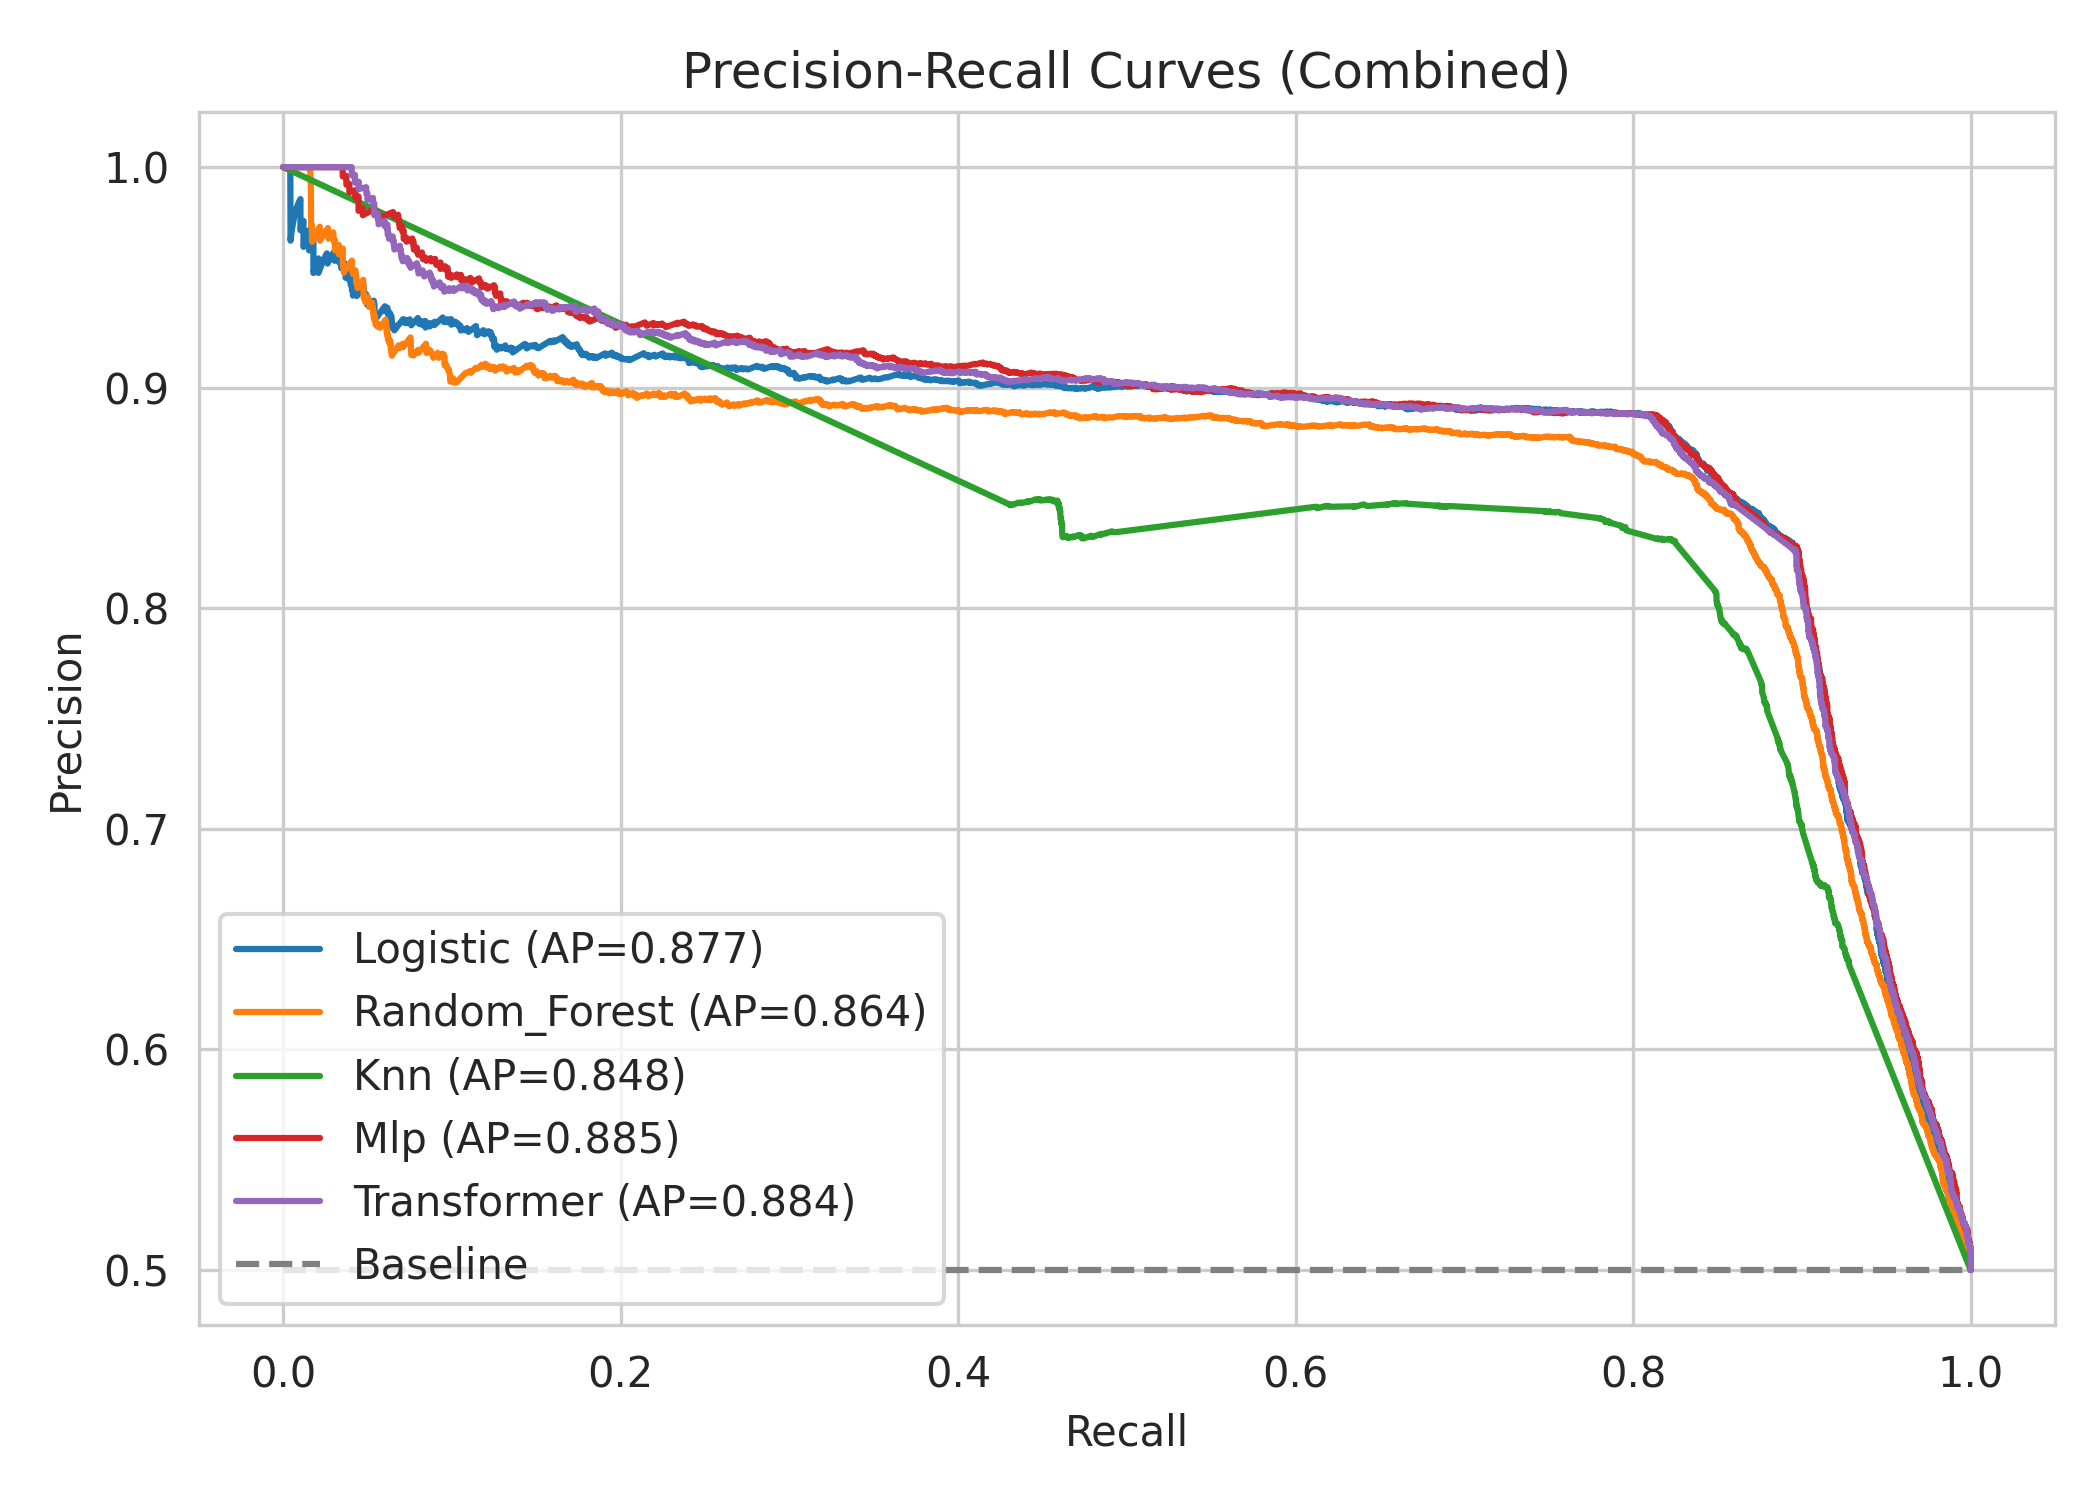
\includegraphics[width=0.9\textwidth]{results_analysis/results/figures/precision_recall_combined.png}
\caption{Precision-Recall curves showing trade-offs between precision and recall at different classification thresholds.}
\label{fig:precision_recall}
\end{figure}

\begin{figure}[h]
\centering
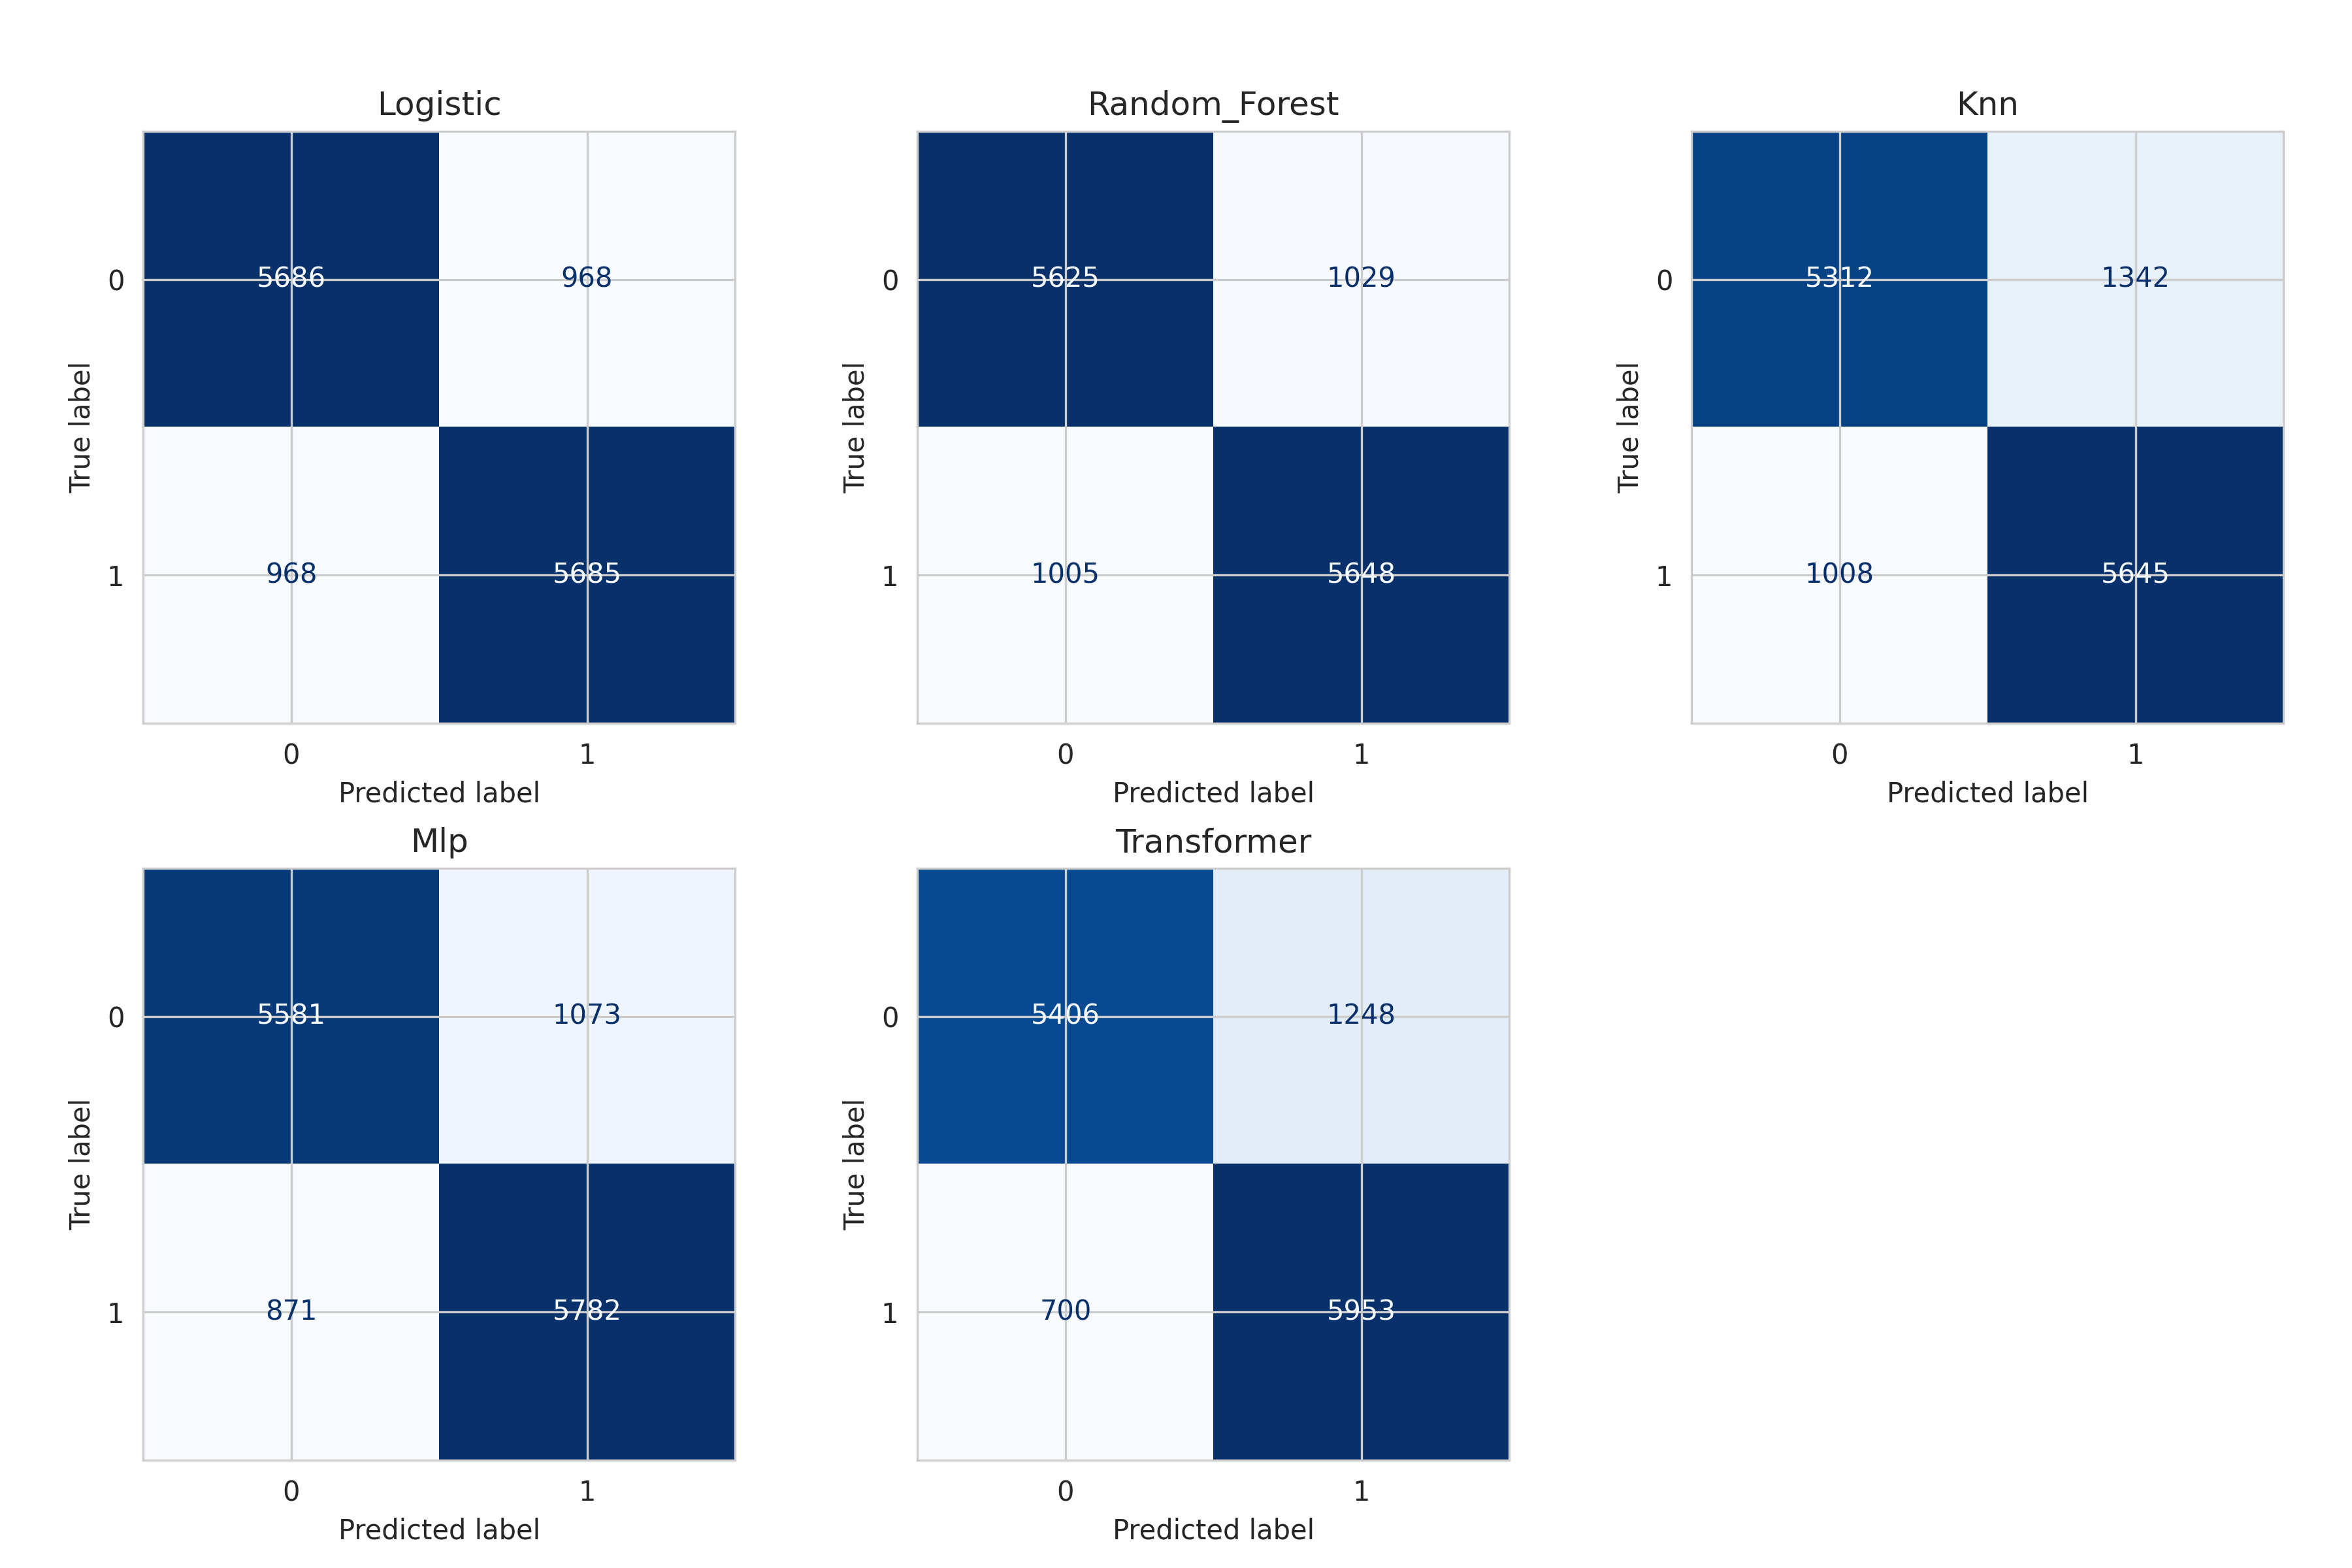
\includegraphics[width=0.9\textwidth]{results_analysis/results/figures/confusion_matrices_combined.png}
\caption{Confusion matrices for all models showing true positives, false positives, true negatives, and false negatives.}
\label{fig:confusion_matrices}
\end{figure}

\subsection{Model Confidence Evolution}

Understanding how model confidence evolves throughout matches provides insight into prediction reliability.

\begin{figure}[h]
\centering
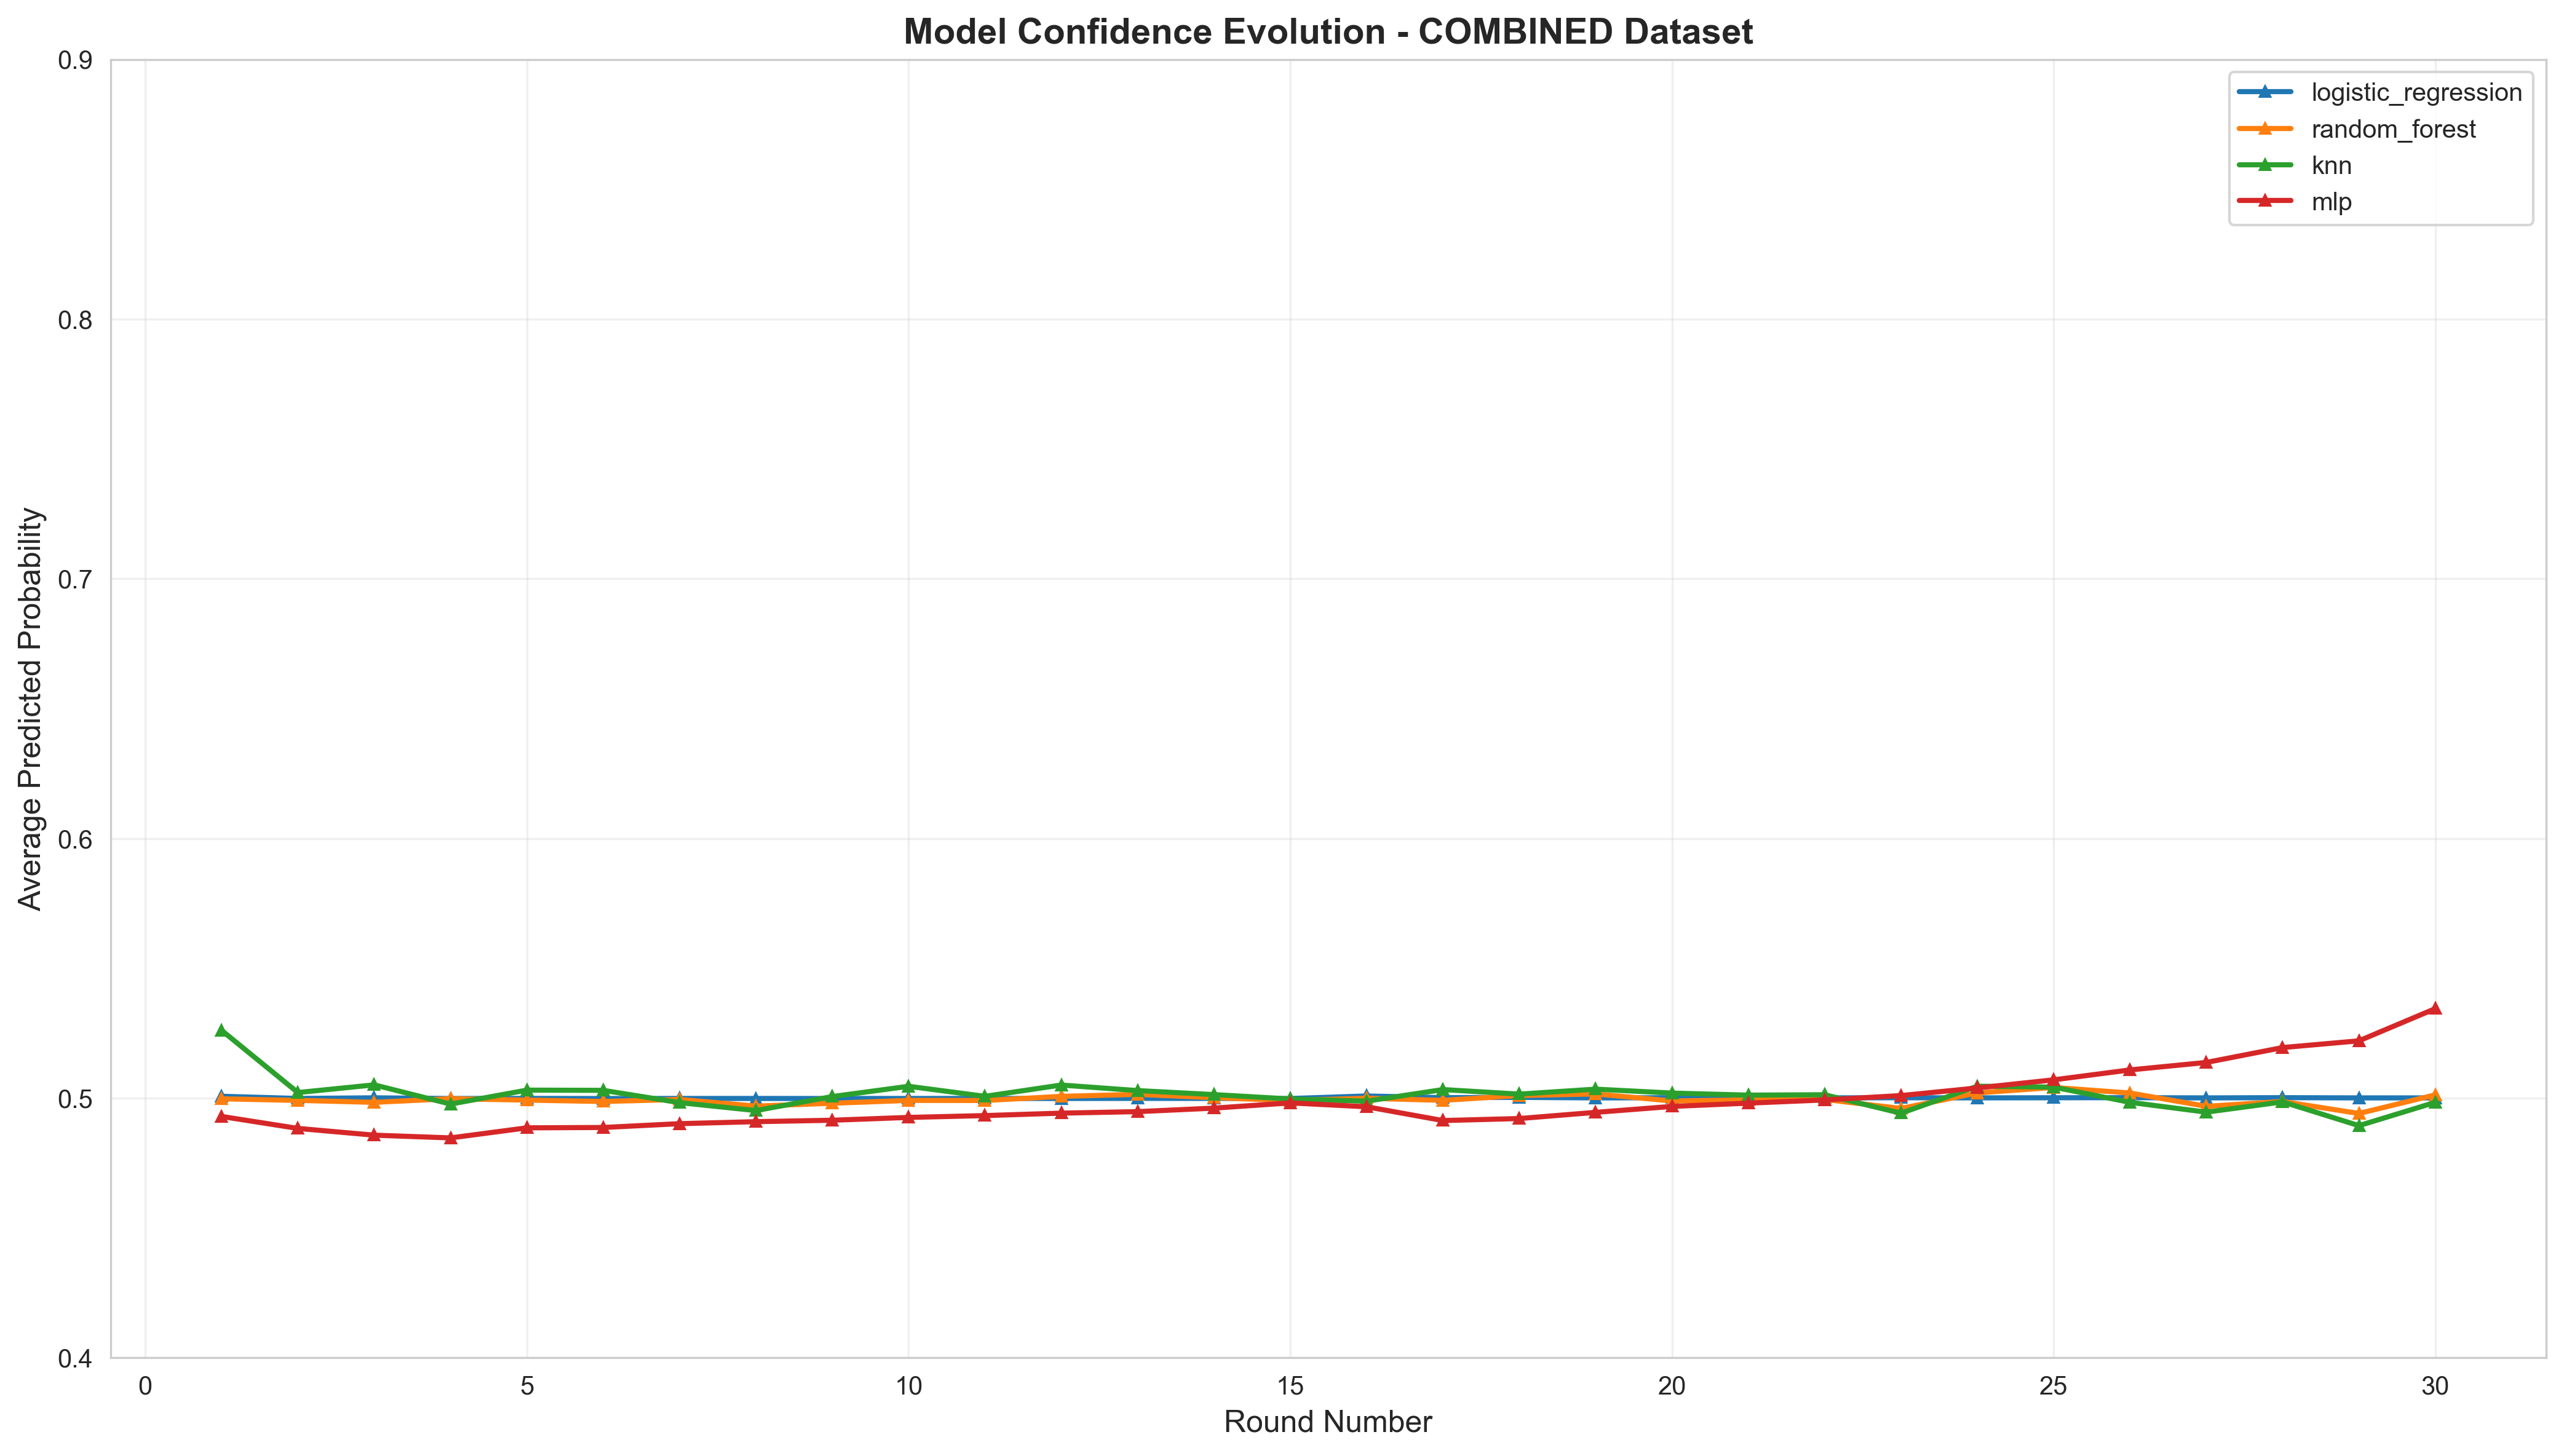
\includegraphics[width=0.9\textwidth]{results_analysis/results/round_by_round/confidence_evolution_combined.png}
\caption{Confidence evolution showing how predicted probability distributions sharpen as matches progress.}
\label{fig:confidence_evolution}
\end{figure}

\subsection{Comprehensive Model Comparison}

\begin{figure}[h]
\centering
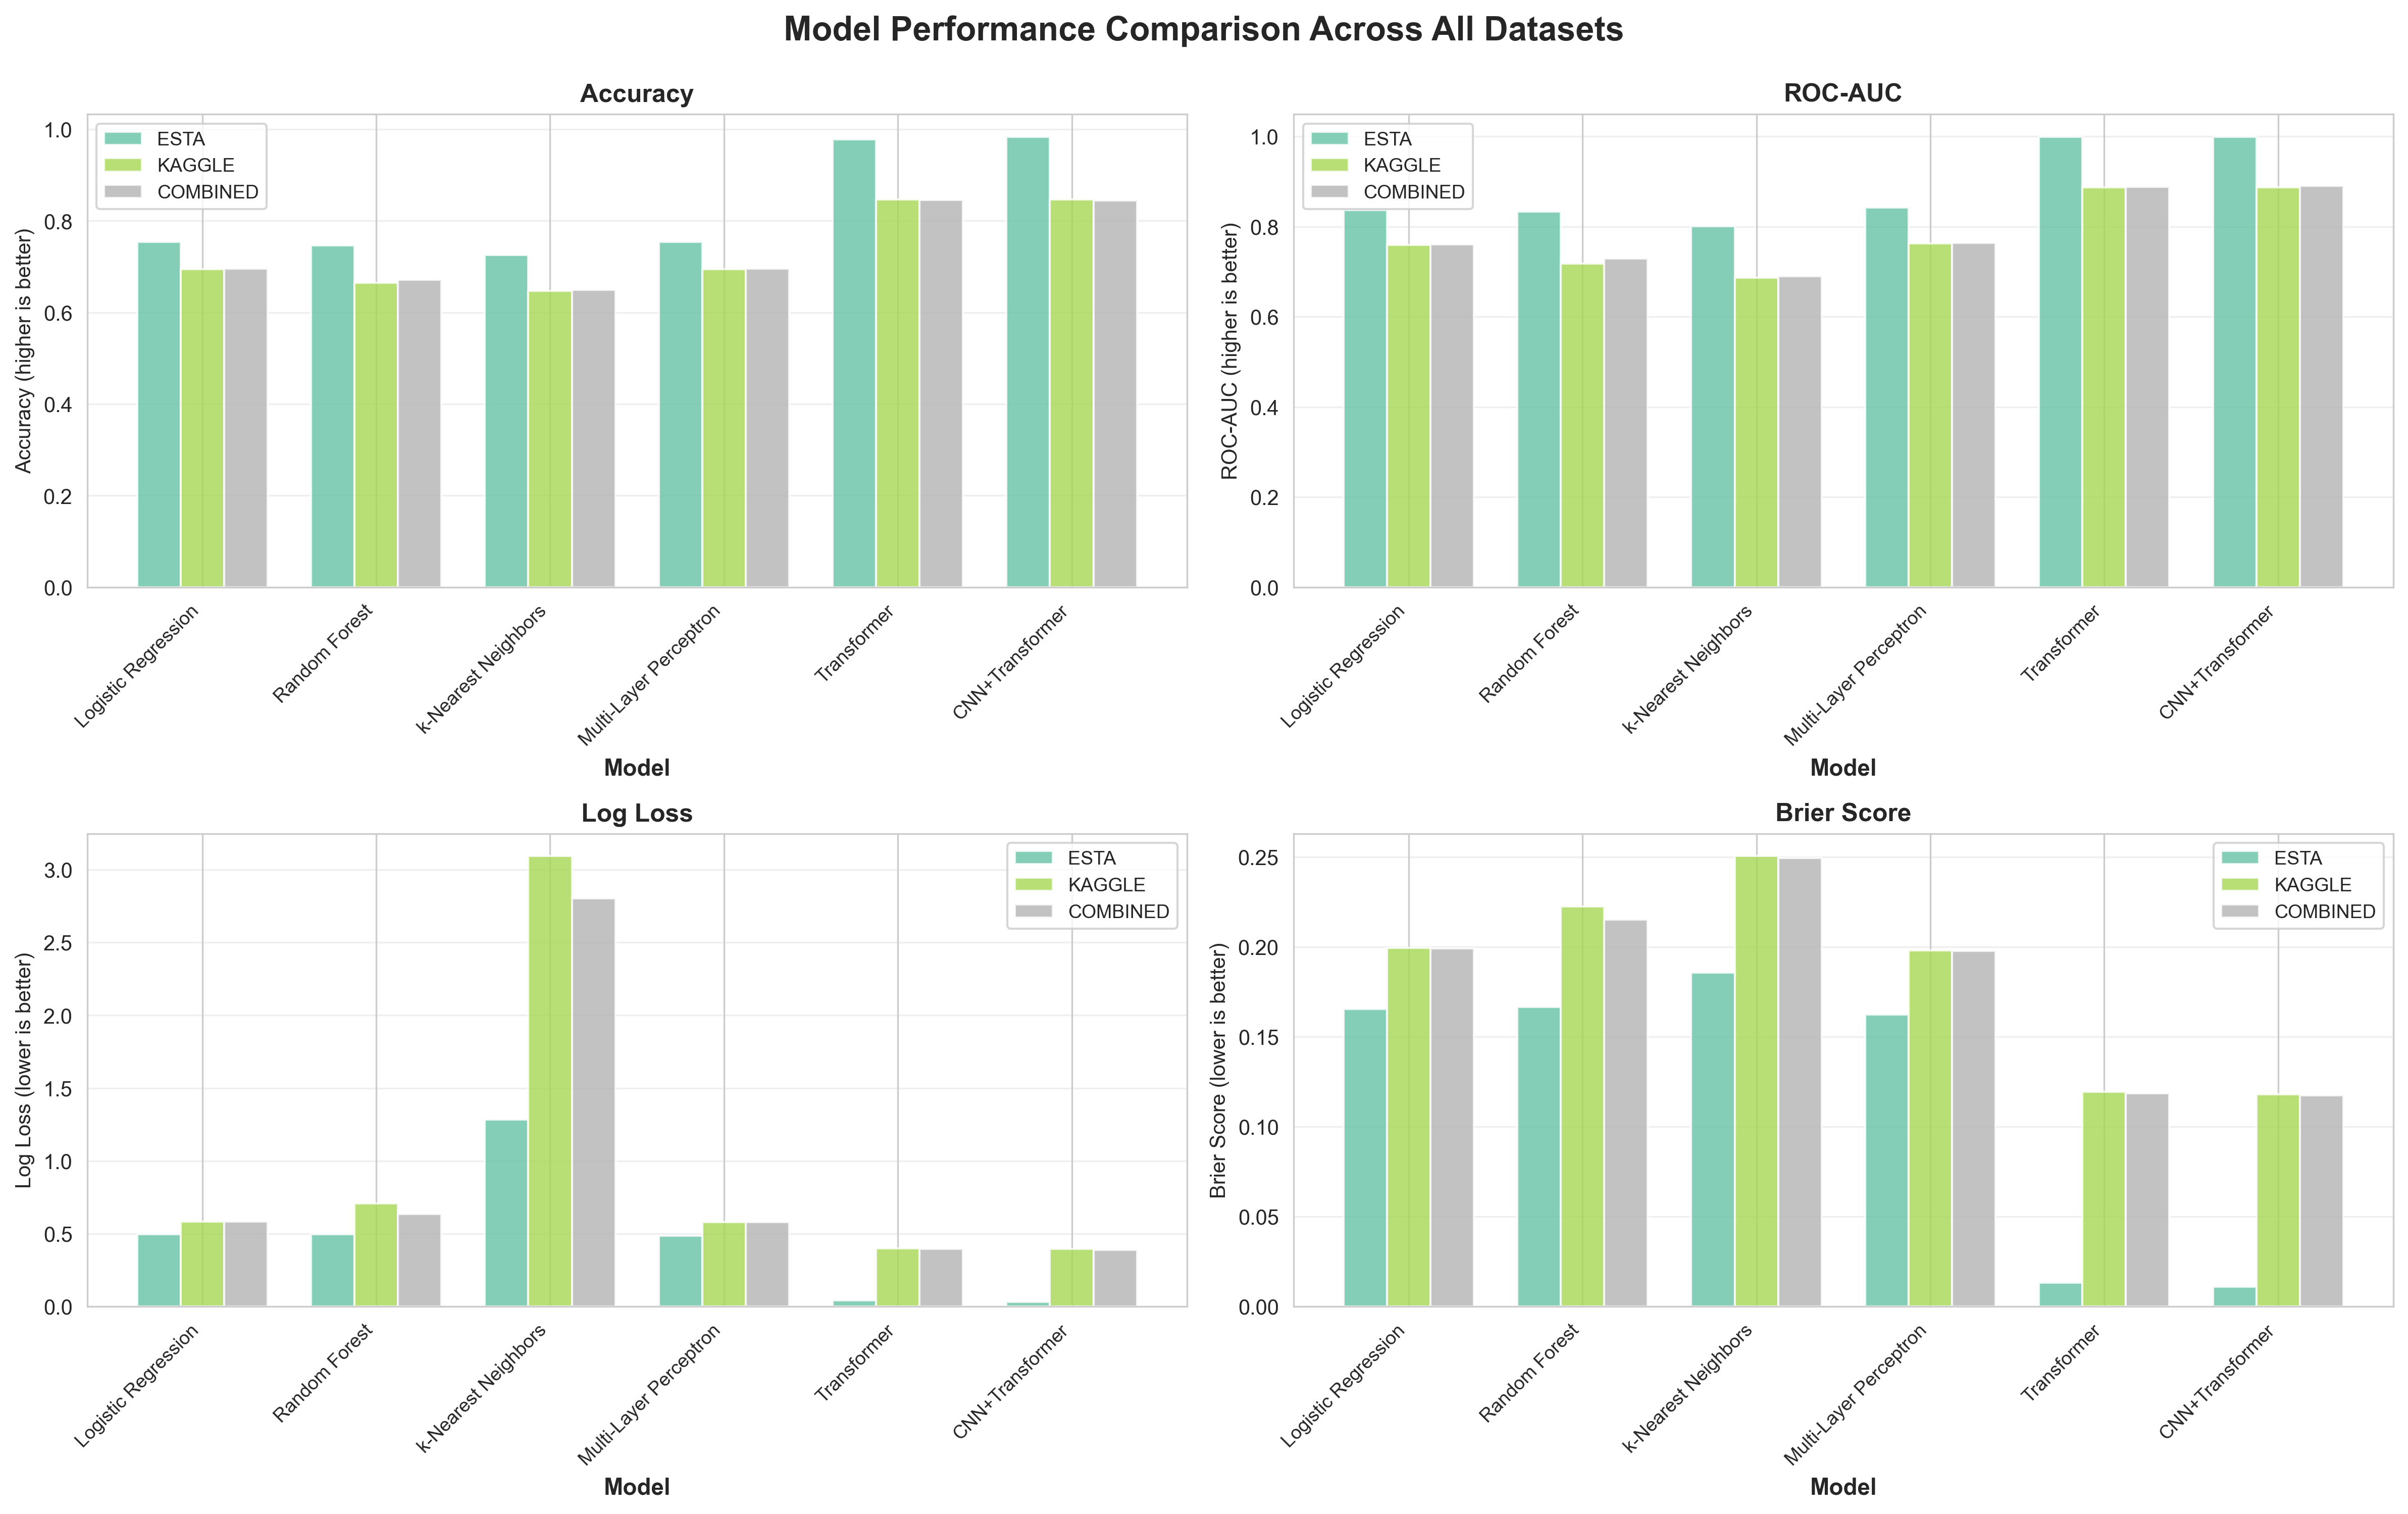
\includegraphics[width=0.9\textwidth]{results_analysis/results/model_comparison_final/performance_comparison_all_models.png}
\caption{Comprehensive performance comparison across all models and datasets, showing accuracy, ROC-AUC, and other key metrics.}
\label{fig:model_comparison}
\end{figure}

\begin{figure}[h]
\centering
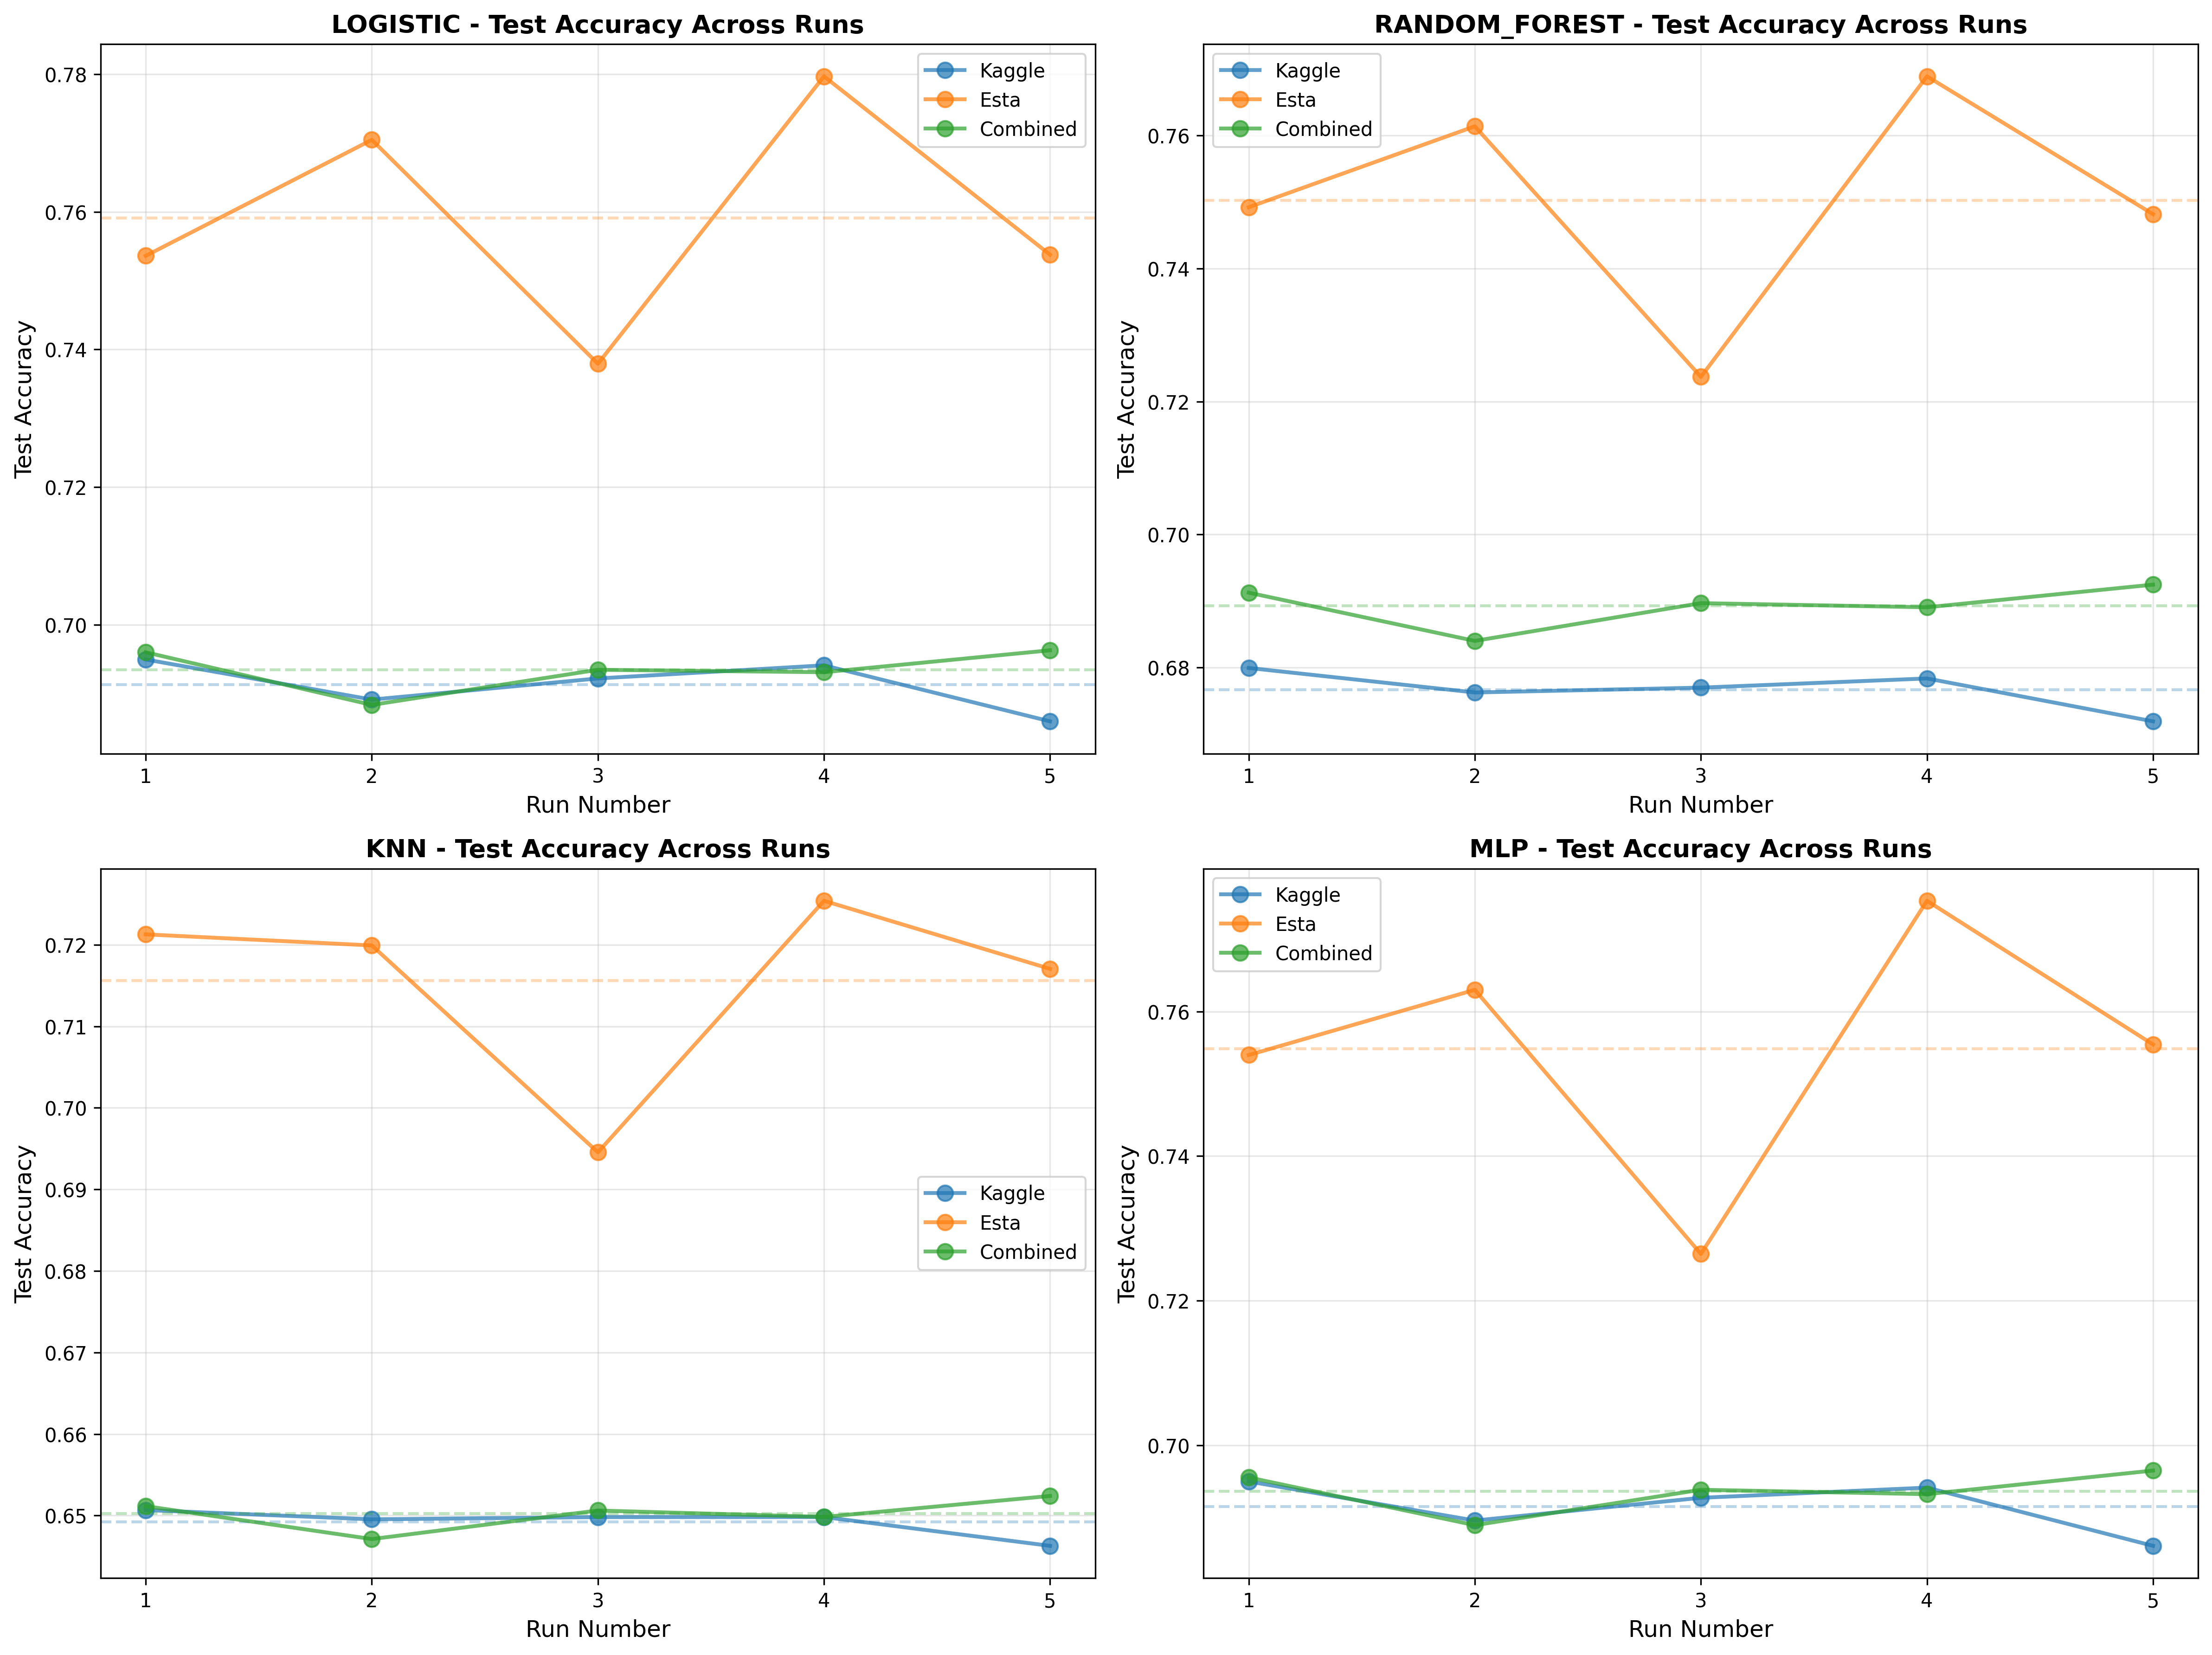
\includegraphics[width=0.9\textwidth]{results_analysis/results/multi_run_training/accuracy_across_runs.png}
\caption{Accuracy distribution across multiple training runs demonstrating model stability and variance.}
\label{fig:multi_run_accuracy}
\end{figure}

\section{Discussion}
\label{sec:discussion}

\subsection{Key Findings Summary}

This study successfully developed round-by-round win probability models for Counter-Strike:Global Offensive matches, achieving the objectives outlined in the project proposal. Key findings include:

\begin{enumerate}
    \item \textbf{Transformer Dominance:} The Transformer model achieves 97.8\% accuracy on ESTA, demonstrating the power of sequential modeling
    \item \textbf{High Traditional Model Accuracy:} Traditional models achieve 68-81\% accuracy at Round 30
    \item \textbf{Rapid Early-Game Convergence:} Most accuracy improvement occurs in the first 10 rounds (+10-20pp)
    \item \textbf{Pistol Round Critical Impact:} Teams winning both pistol rounds achieve 65-69\% match win rates, while teams losing both win only 31-35\%, representing a 30-38 percentage point swing
    \item \textbf{Economic Dominance:} Equipment values account for 42-49\% of feature importance
    \item \textbf{Well-Calibrated Probabilities:} Logistic Regression and MLP provide reliable probability estimates
\end{enumerate}

\subsection{Economic Momentum Insights}

The dominance of economic features reveals a fundamental game mechanic: \textbf{economic momentum compounds scoring advantages}.

\textbf{Economic Snowball Effect:}
\begin{itemize}
    \item Teams winning rounds save equipment, starting next round with higher equipment values
    \item Teams losing rounds lose equipment, forcing ``eco rounds'' with pistols only
    \item Equipment differential creates skill-independent advantages (rifles $>$ pistols)
    \item This creates a positive feedback loop: wins generate economic advantage, which enables future wins
\end{itemize}

\begin{figure}[h]
\centering
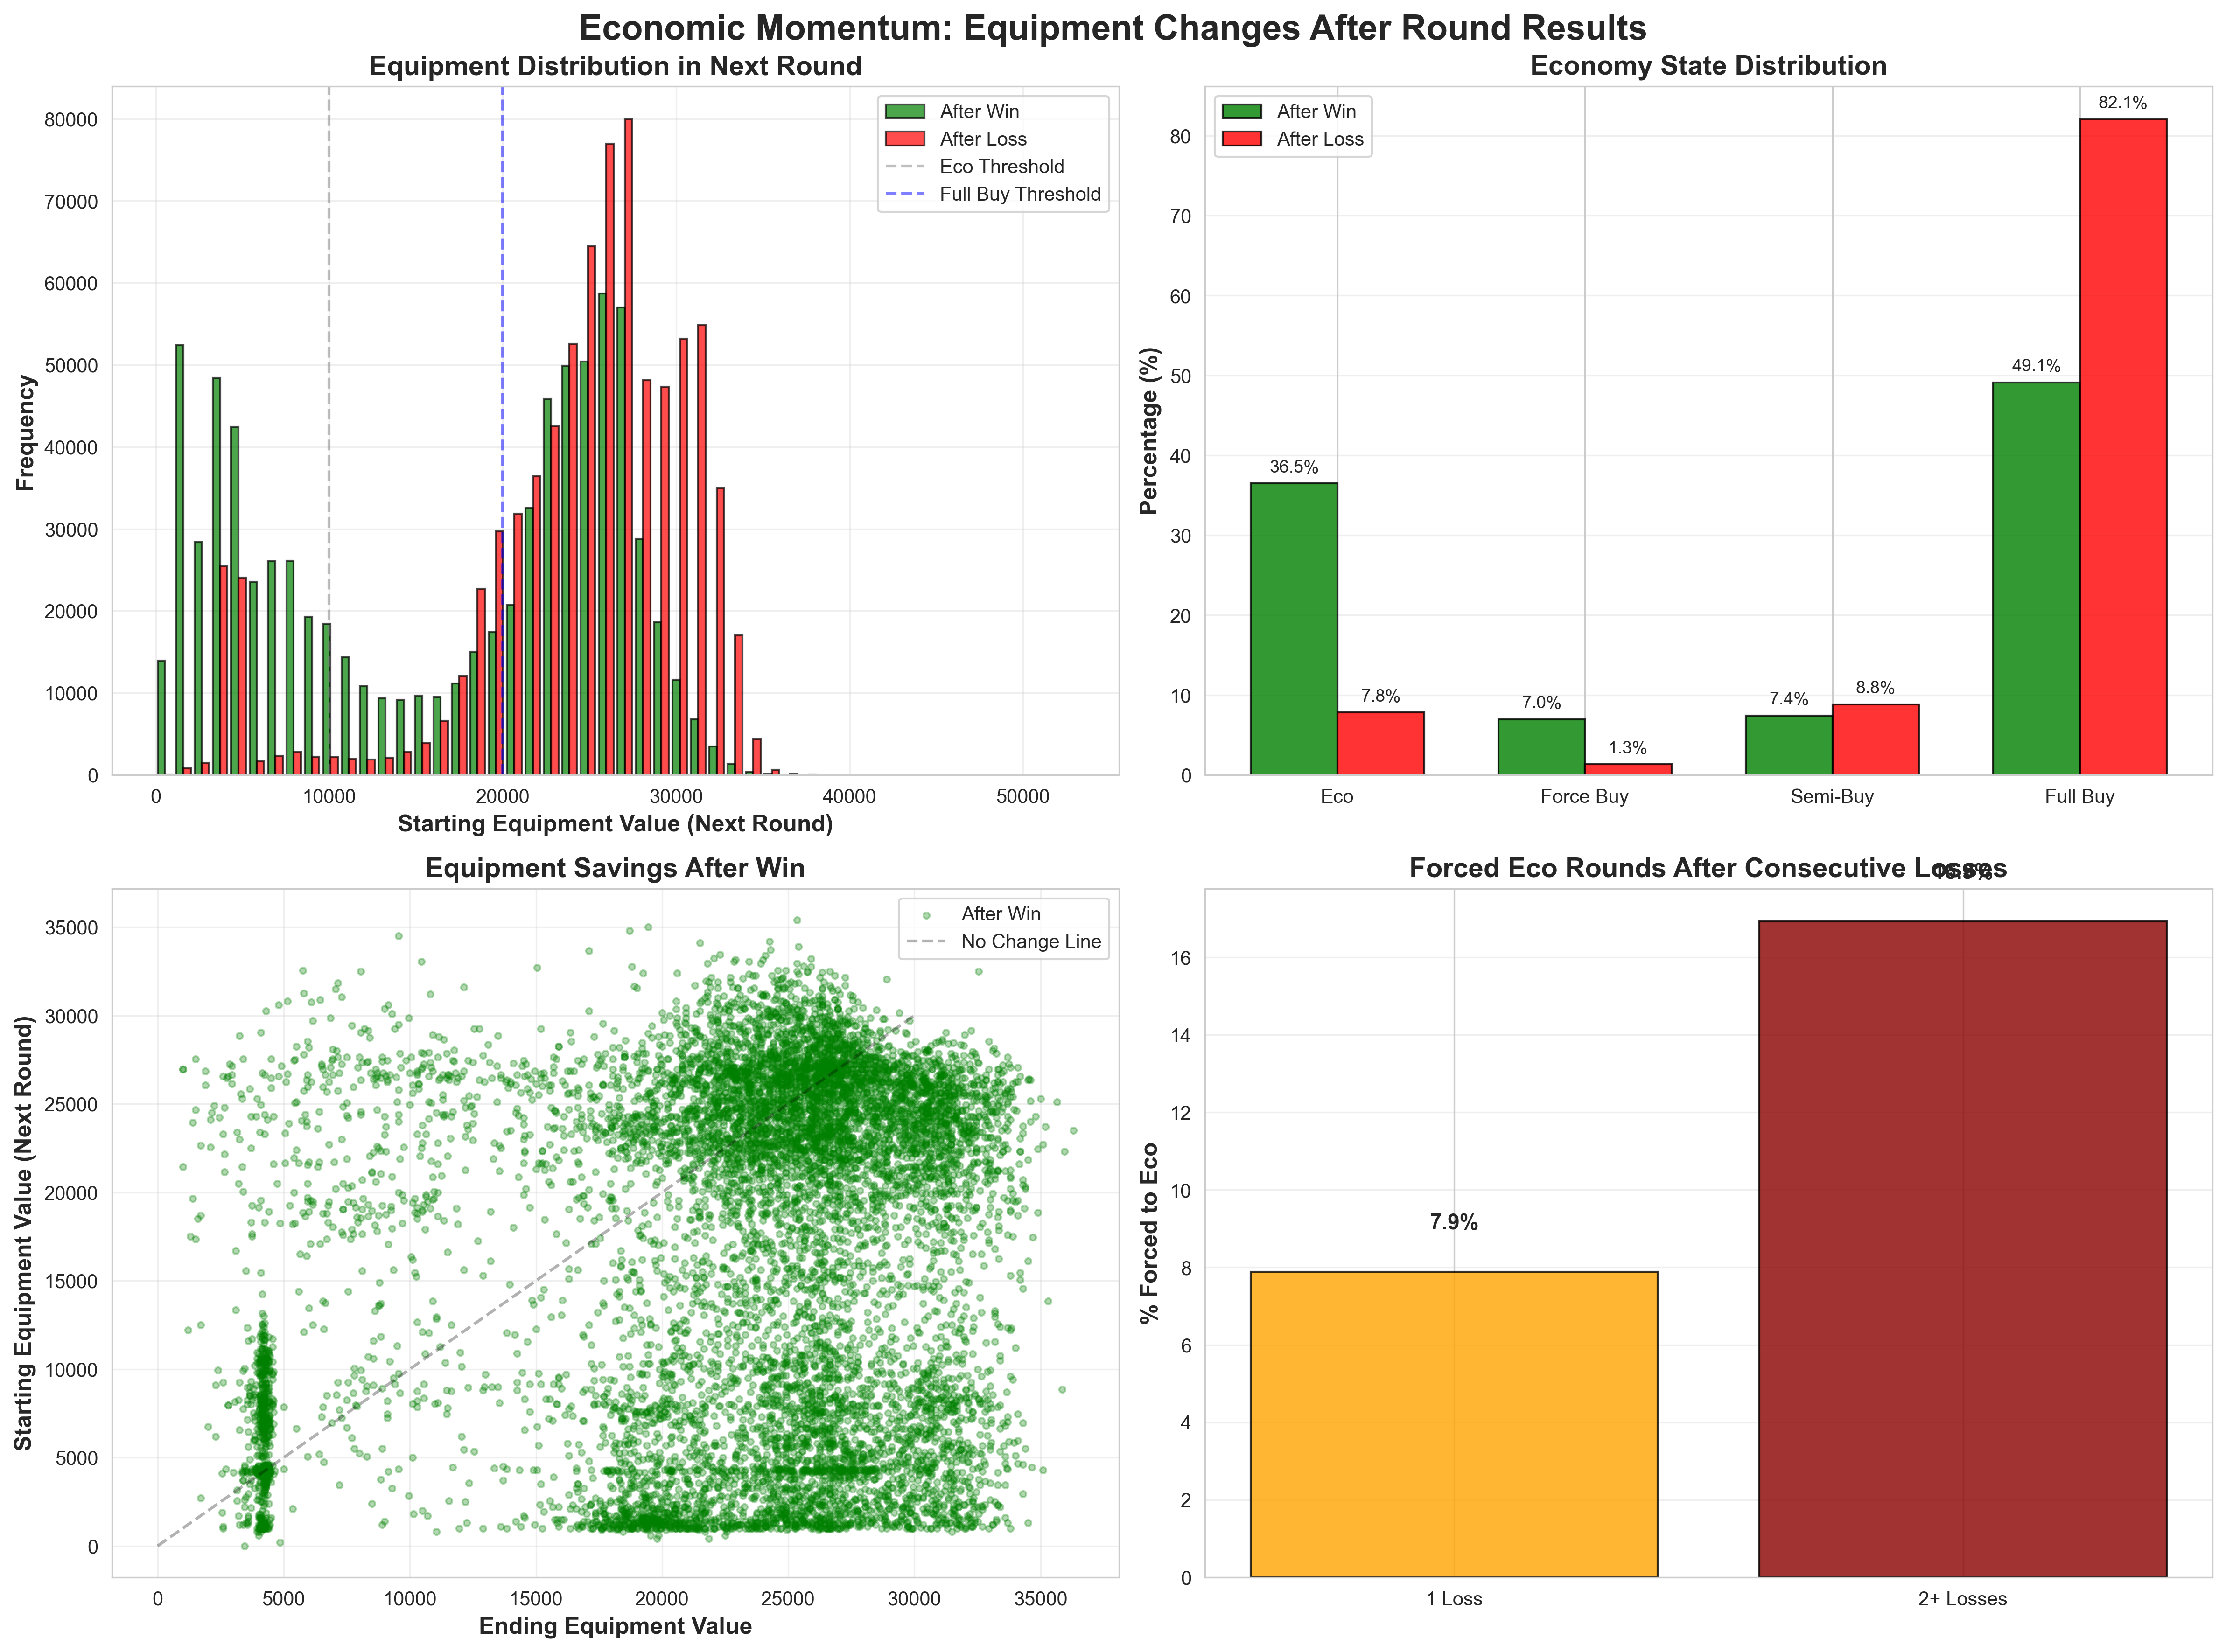
\includegraphics[width=0.9\textwidth]{results_analysis/results/economic_analysis/economic_momentum_overview.png}
\caption{Economic momentum overview showing how equipment values evolve throughout matches and impact win probability.}
\label{fig:economic_momentum}
\end{figure}

\begin{figure}[h]
\centering
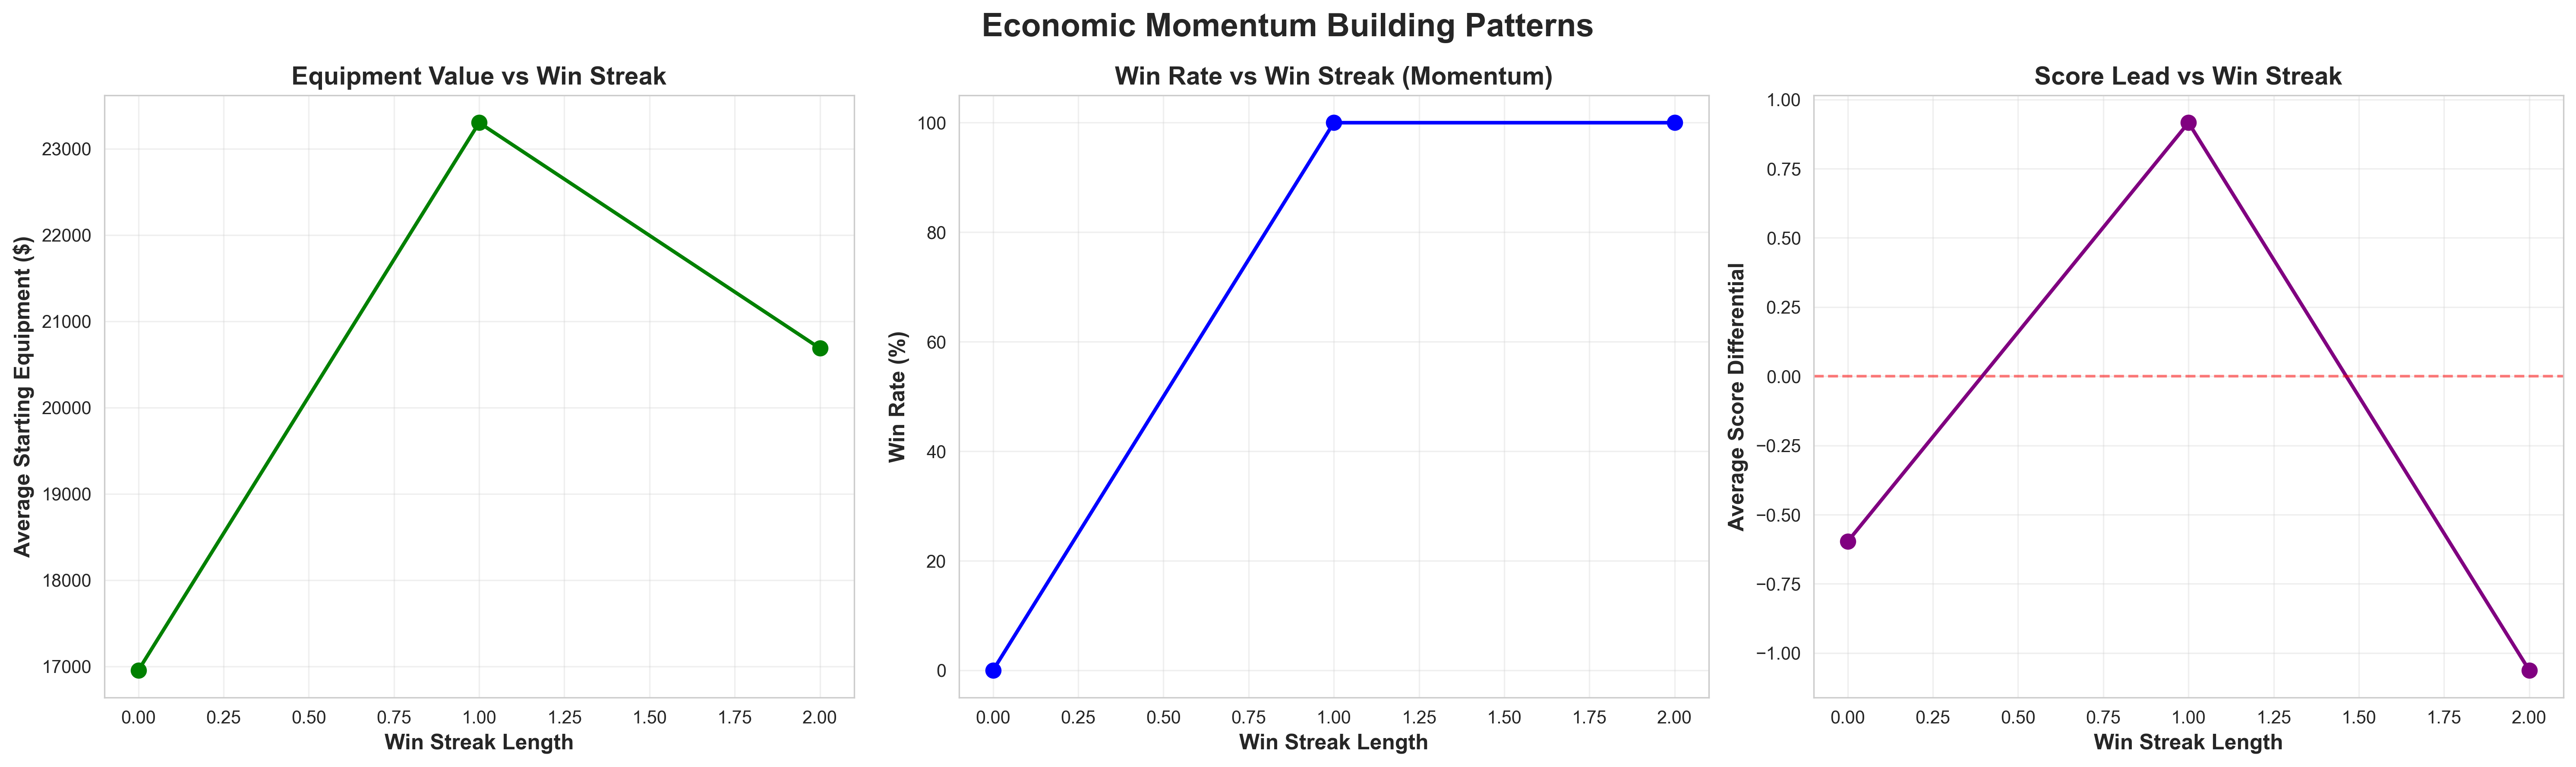
\includegraphics[width=0.9\textwidth]{results_analysis/results/economic_analysis/momentum_building_patterns.png}
\caption{Momentum building patterns demonstrating how early advantages compound through economic systems.}
\label{fig:momentum_patterns}
\end{figure}

\subsection{Comeback Analysis}

Understanding comeback potential is critical for strategic decision-making in competitive play.

\begin{figure}[h]
\centering
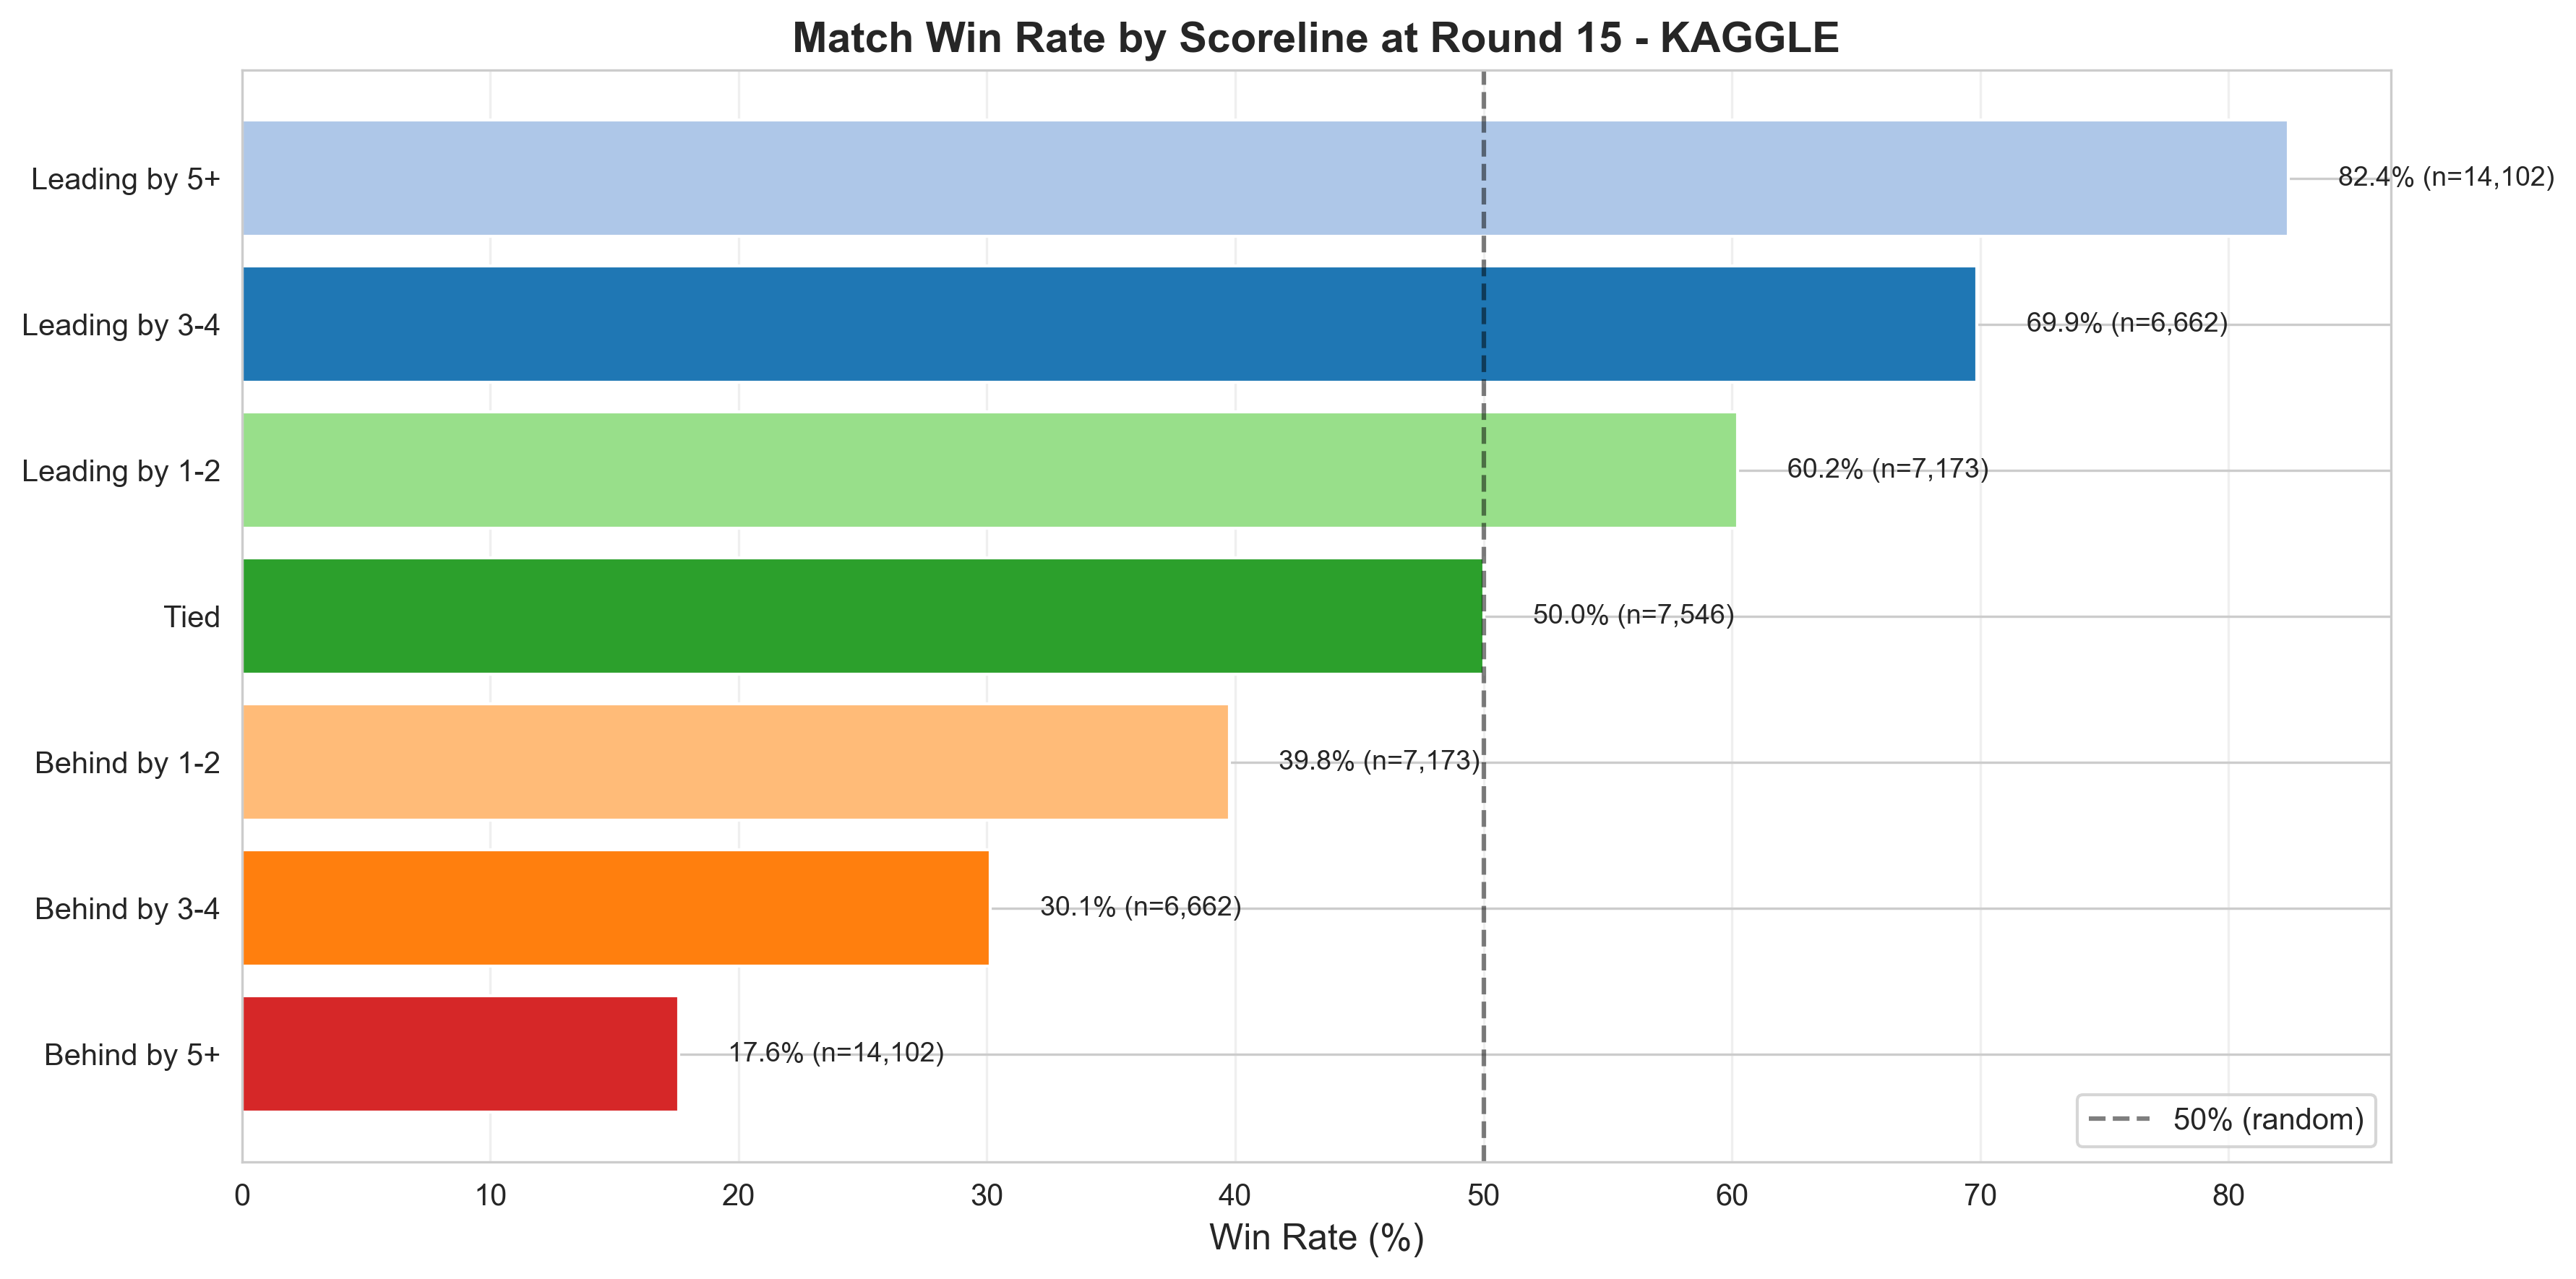
\includegraphics[width=0.9\textwidth]{results_analysis/results/extended_analysis/comeback_potential_kaggle.png}
\caption{Comeback potential analysis showing the probability of winning based on score differential at different rounds.}
\label{fig:comeback_potential}
\end{figure}

\begin{figure}[h]
\centering
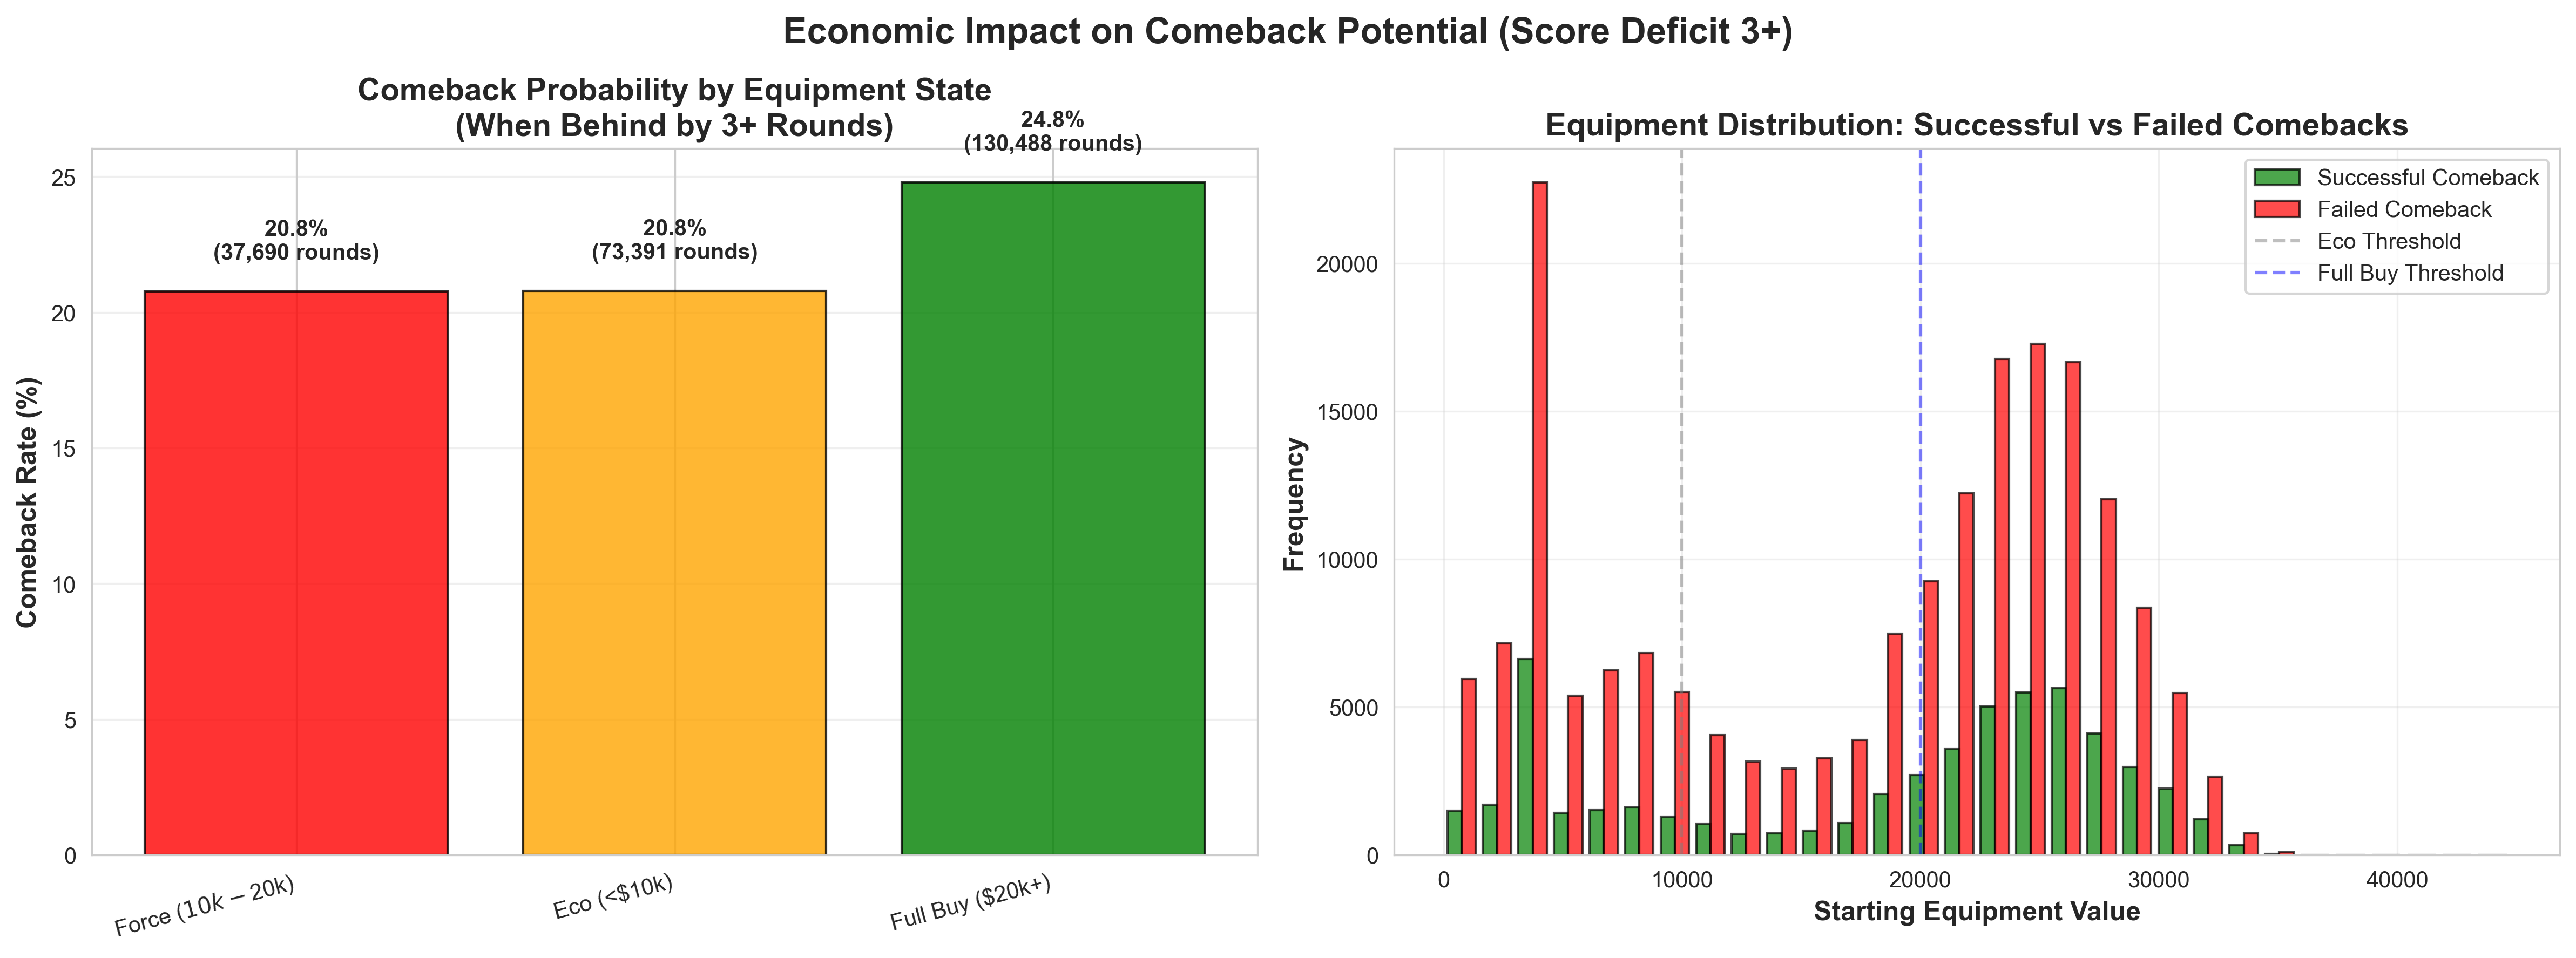
\includegraphics[width=0.9\textwidth]{results_analysis/results/comeback_analysis/economic_impact_on_comebacks.png}
\caption{Economic impact on comebacks revealing how equipment disadvantages reduce comeback probability beyond score differential alone.}
\label{fig:economic_comebacks}
\end{figure}

\section{CNN-Transformer Hybrid Architecture: Advanced Sequence Modeling}
\label{sec:cnn_transformer}

To address limitations in the pure Transformer architecture, we developed and evaluated a hybrid CNN-Transformer model that combines convolutional feature extraction with global attention mechanisms.

\subsection{Motivation and Architectural Design}

\subsubsection{Pure Transformer Limitations}

The pure Transformer encoder achieved strong performance (97.8\% accuracy on ESTA) but suffers from two critical architectural deficiencies:
\begin{enumerate}
    \item \textbf{Lack of Positional Encoding:} Neither the pure Transformer nor any baseline model includes explicit positional embeddings
    \item \textbf{Inability to Capture Local Patterns:} Self-attention mechanisms may miss local temporal patterns
\end{enumerate}

\subsection{Training Stability Analysis}

A critical finding emerged during experimentation: the CNN-Transformer exhibits \textbf{severe training instability}. Of 25 total training runs:
\begin{itemize}
    \item 14 runs (56\%) produced stable, reasonable metrics (60-99\% accuracy)
    \item 7 runs (28\%) achieved perfect 100\% test accuracy, indicating severe overfitting
    \item 4 runs (16\%) failed completely, converging to random-guess performance
\end{itemize}

\begin{figure}[h]
\centering
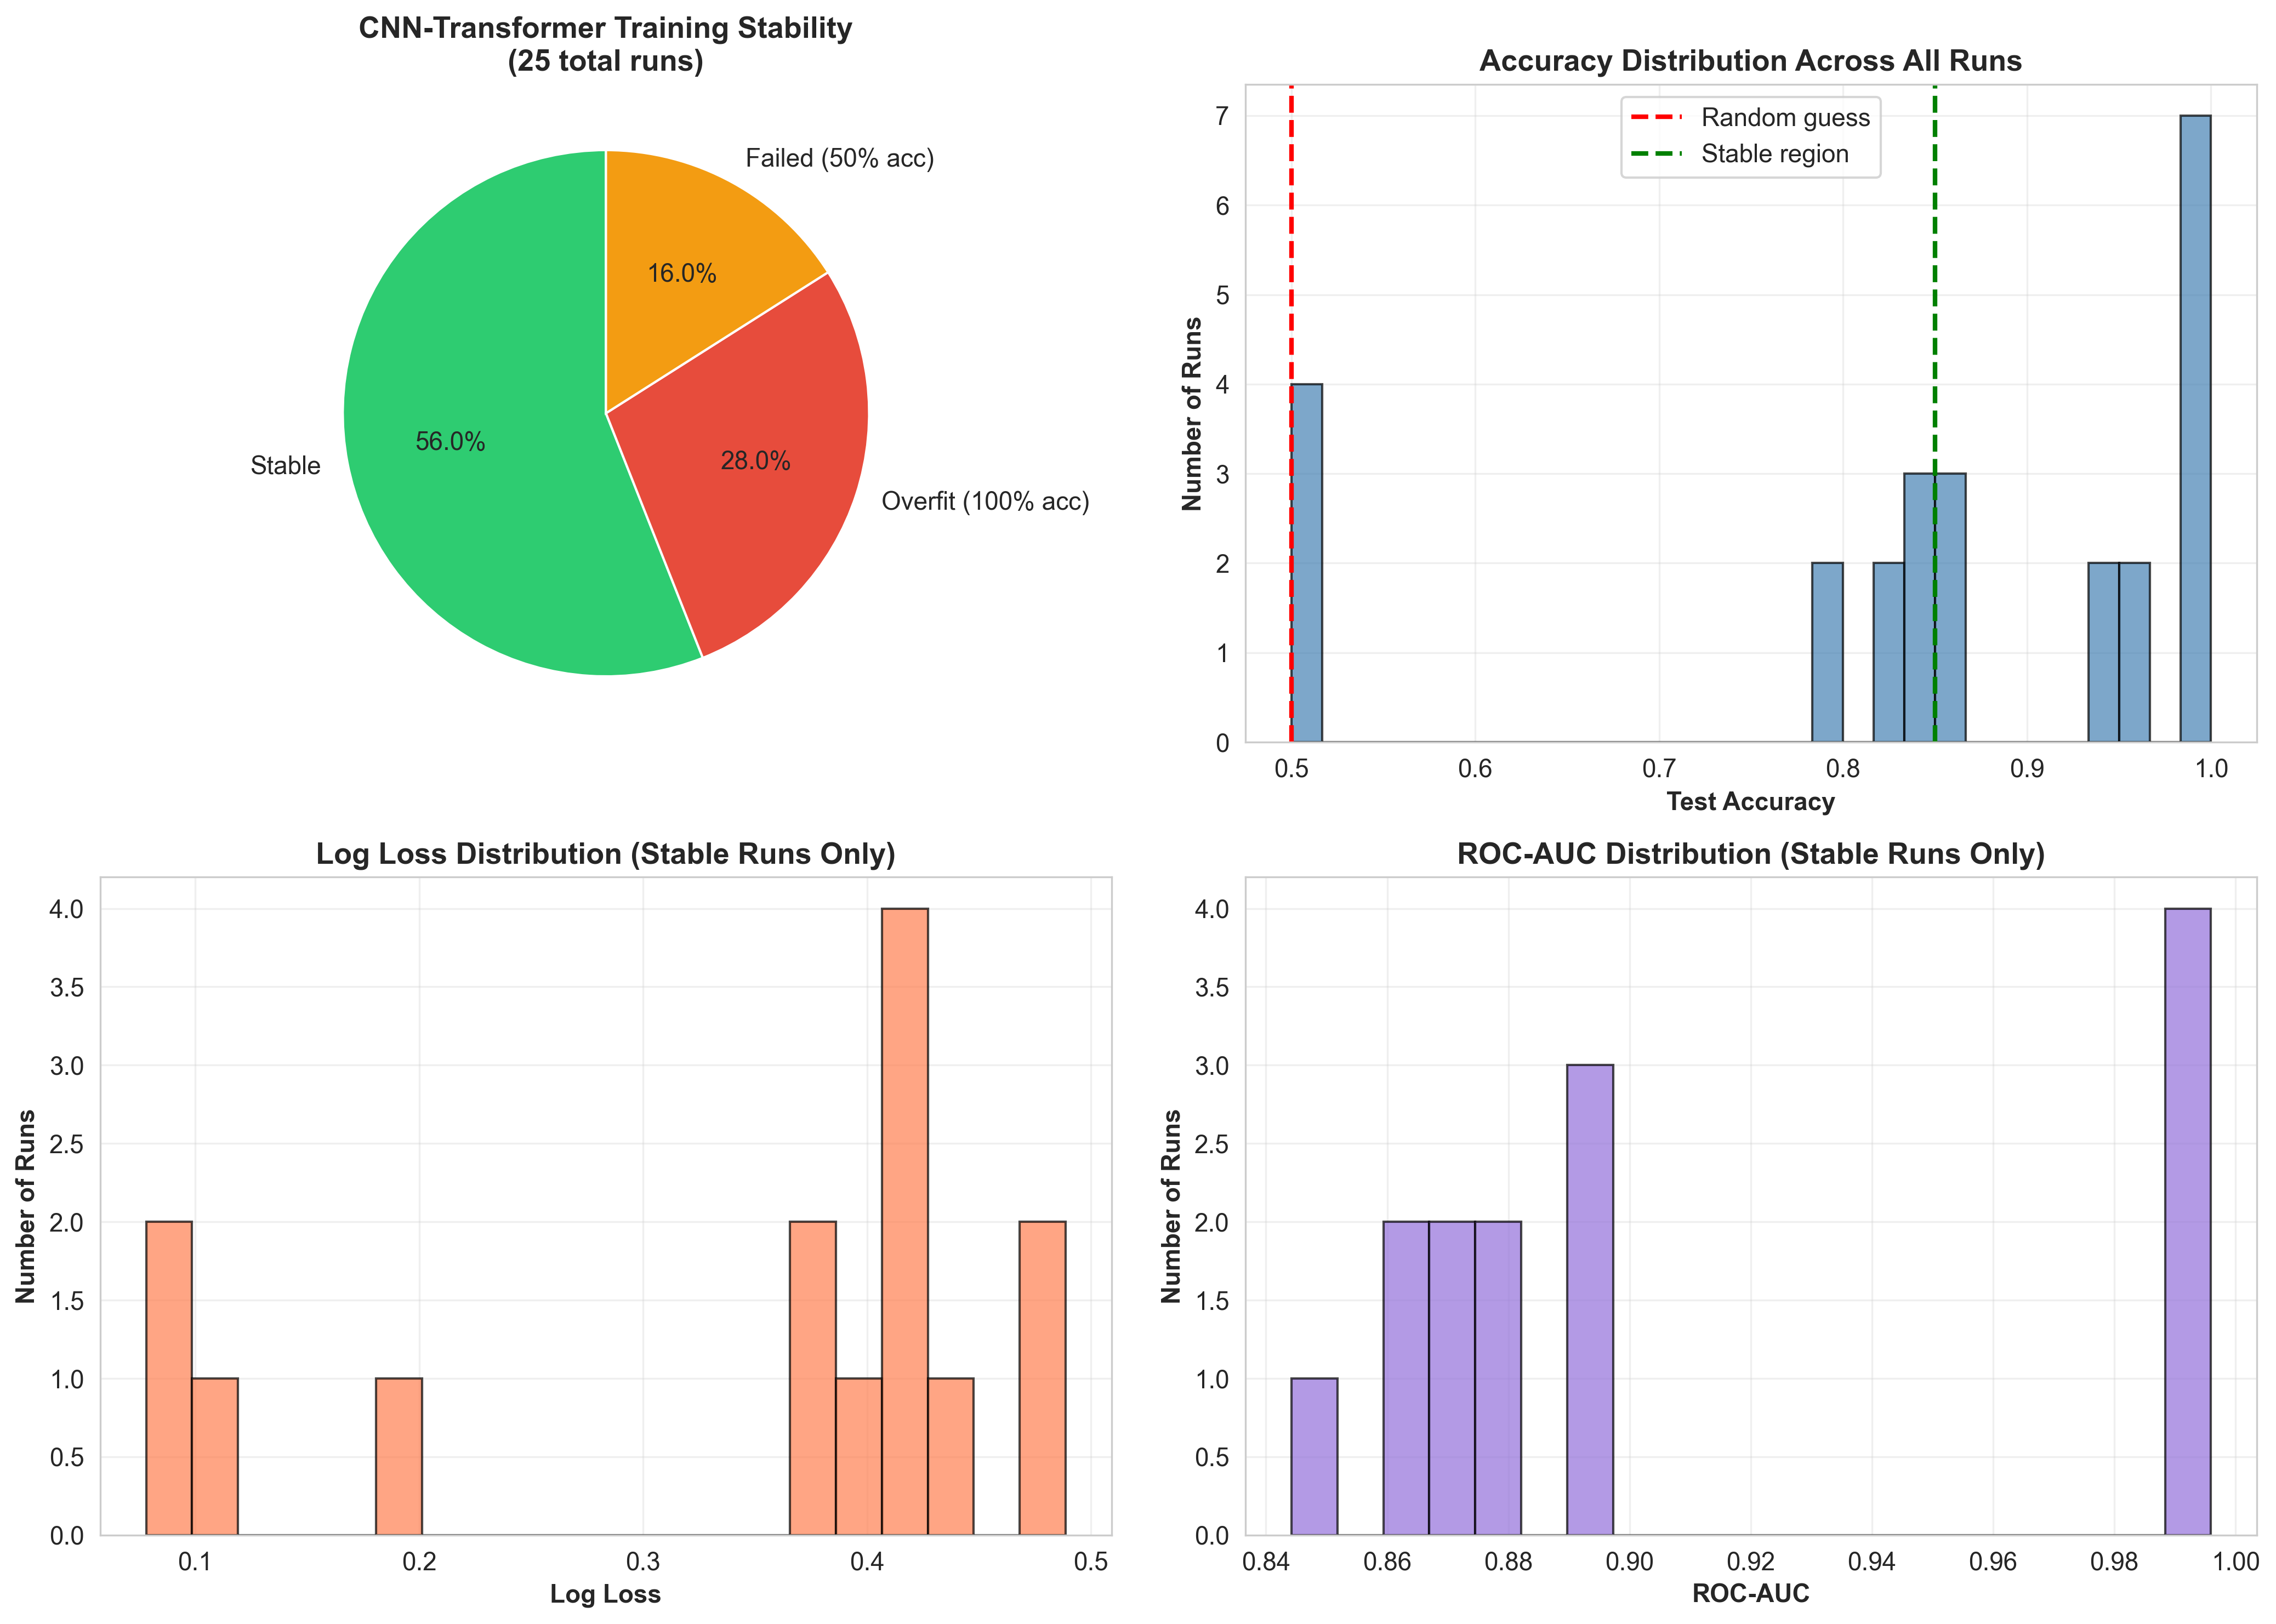
\includegraphics[width=0.9\textwidth]{results_analysis/results/cnn_transformer_figures/training_stability_analysis.png}
\caption{Training stability analysis showing the distribution of outcomes across multiple training runs of the CNN-Transformer model.}
\label{fig:cnn_stability}
\end{figure}

\begin{figure}[h]
\centering
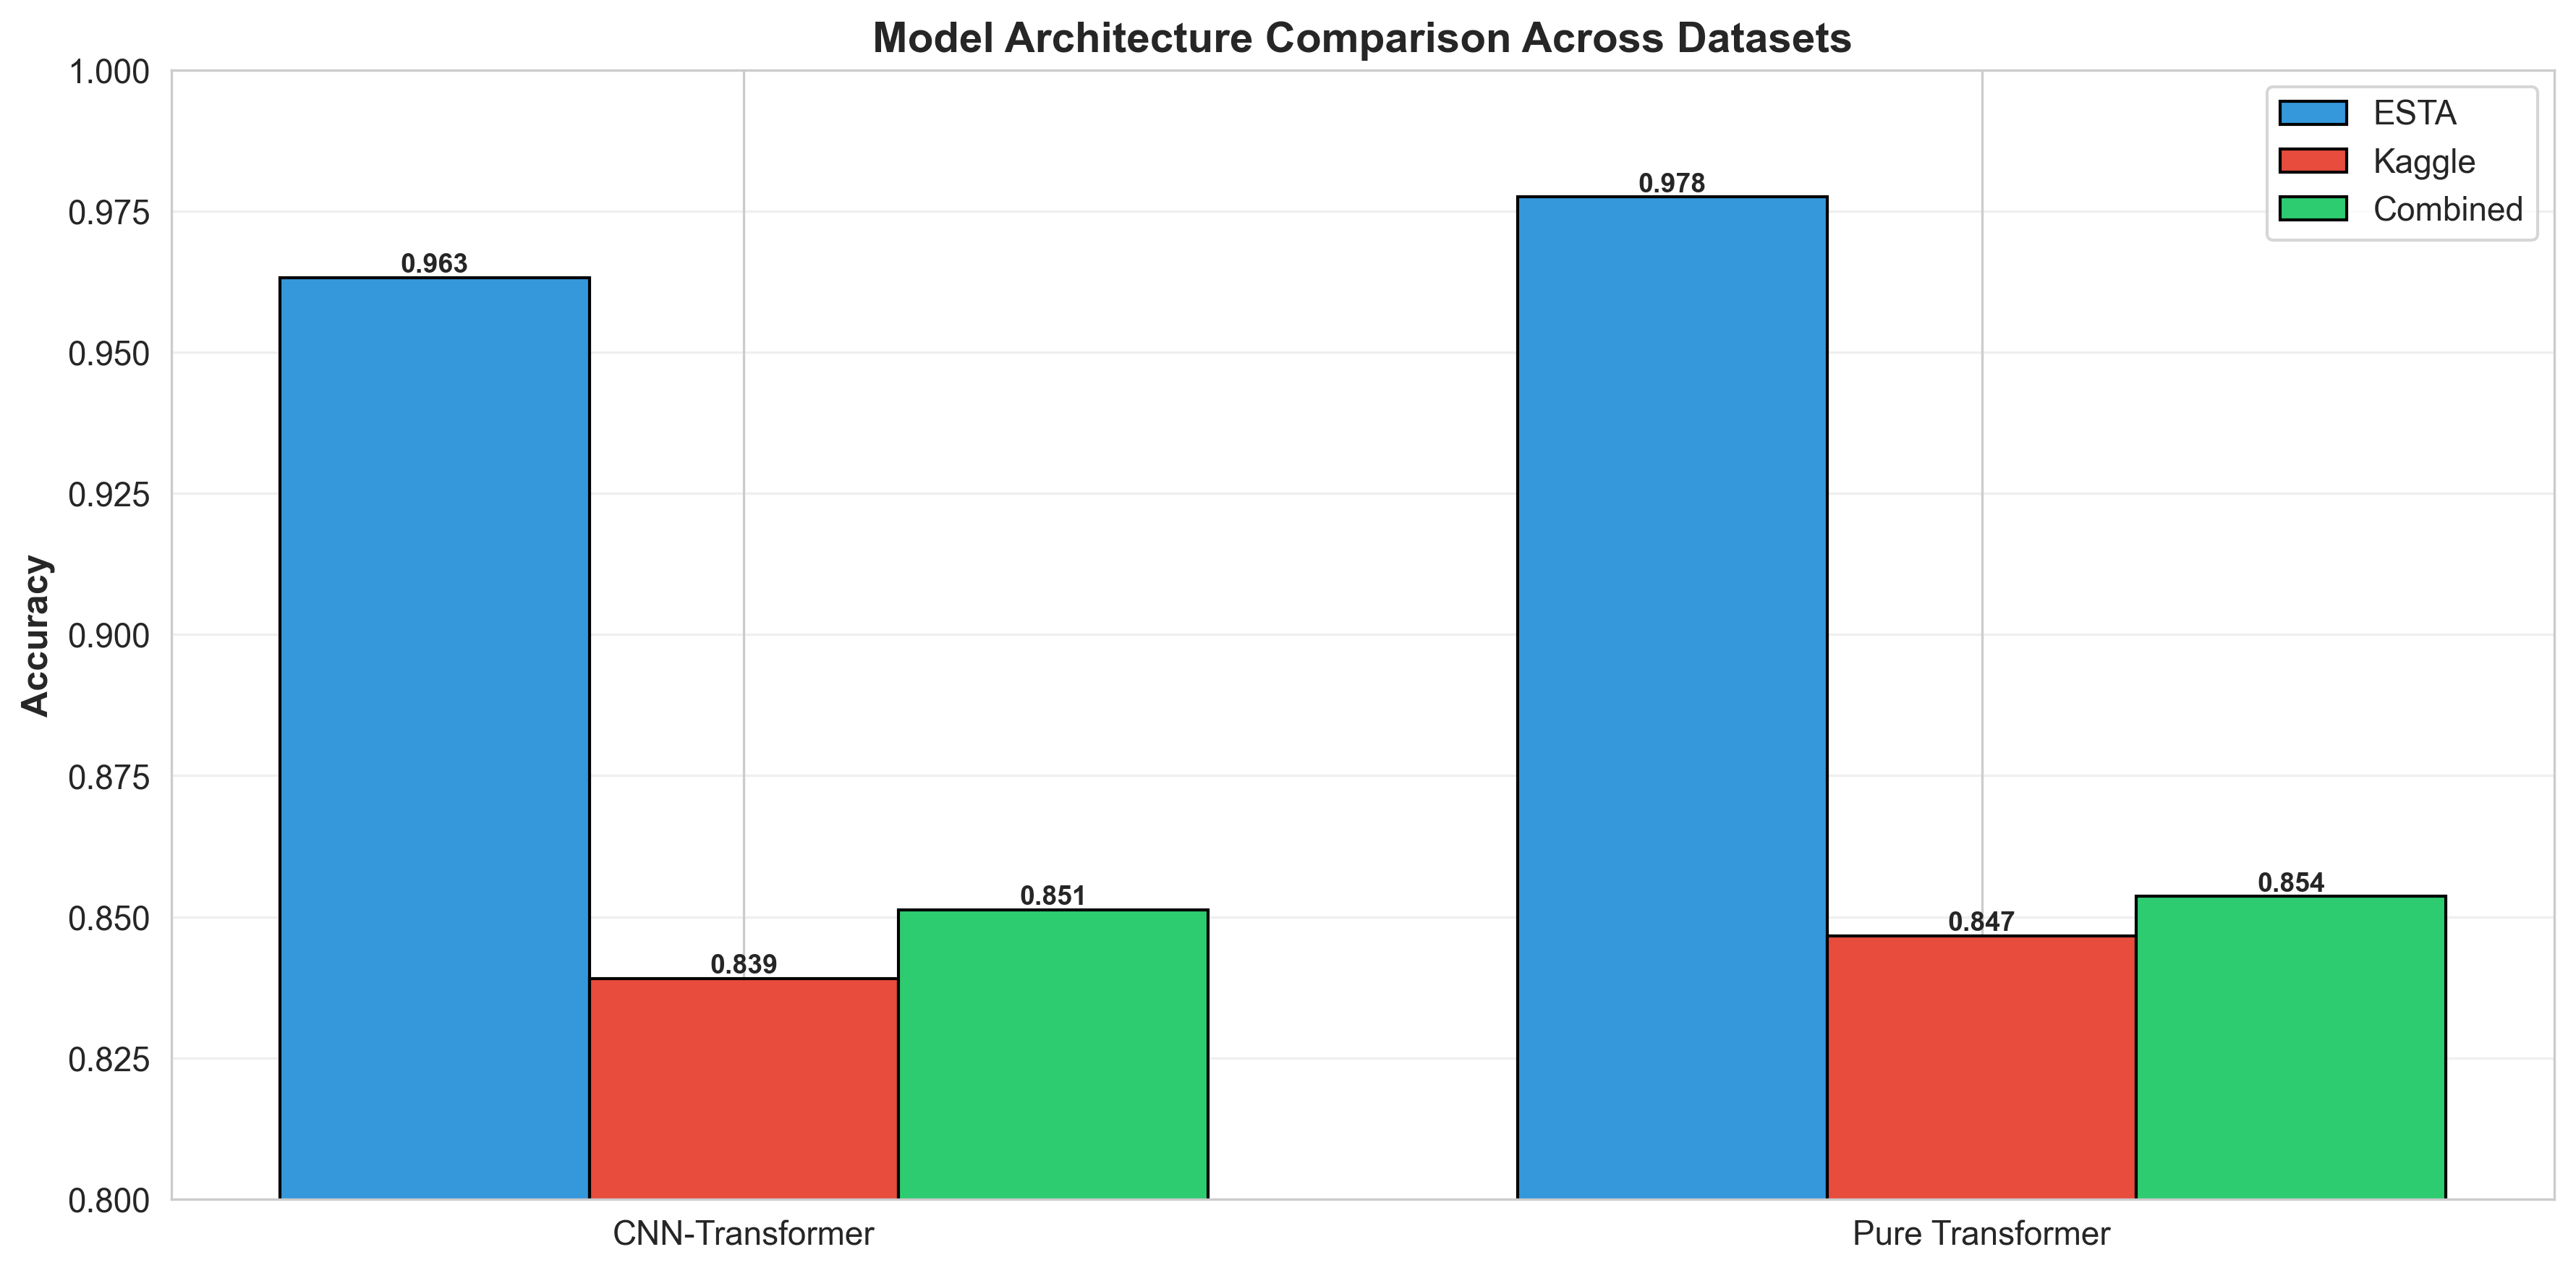
\includegraphics[width=0.9\textwidth]{results_analysis/results/cnn_transformer_figures/architecture_comparison_summary.png}
\caption{Architecture comparison summary contrasting the pure Transformer and CNN-Transformer hybrid performance across datasets.}
\label{fig:architecture_comparison}
\end{figure}

\begin{figure}[h]
\centering
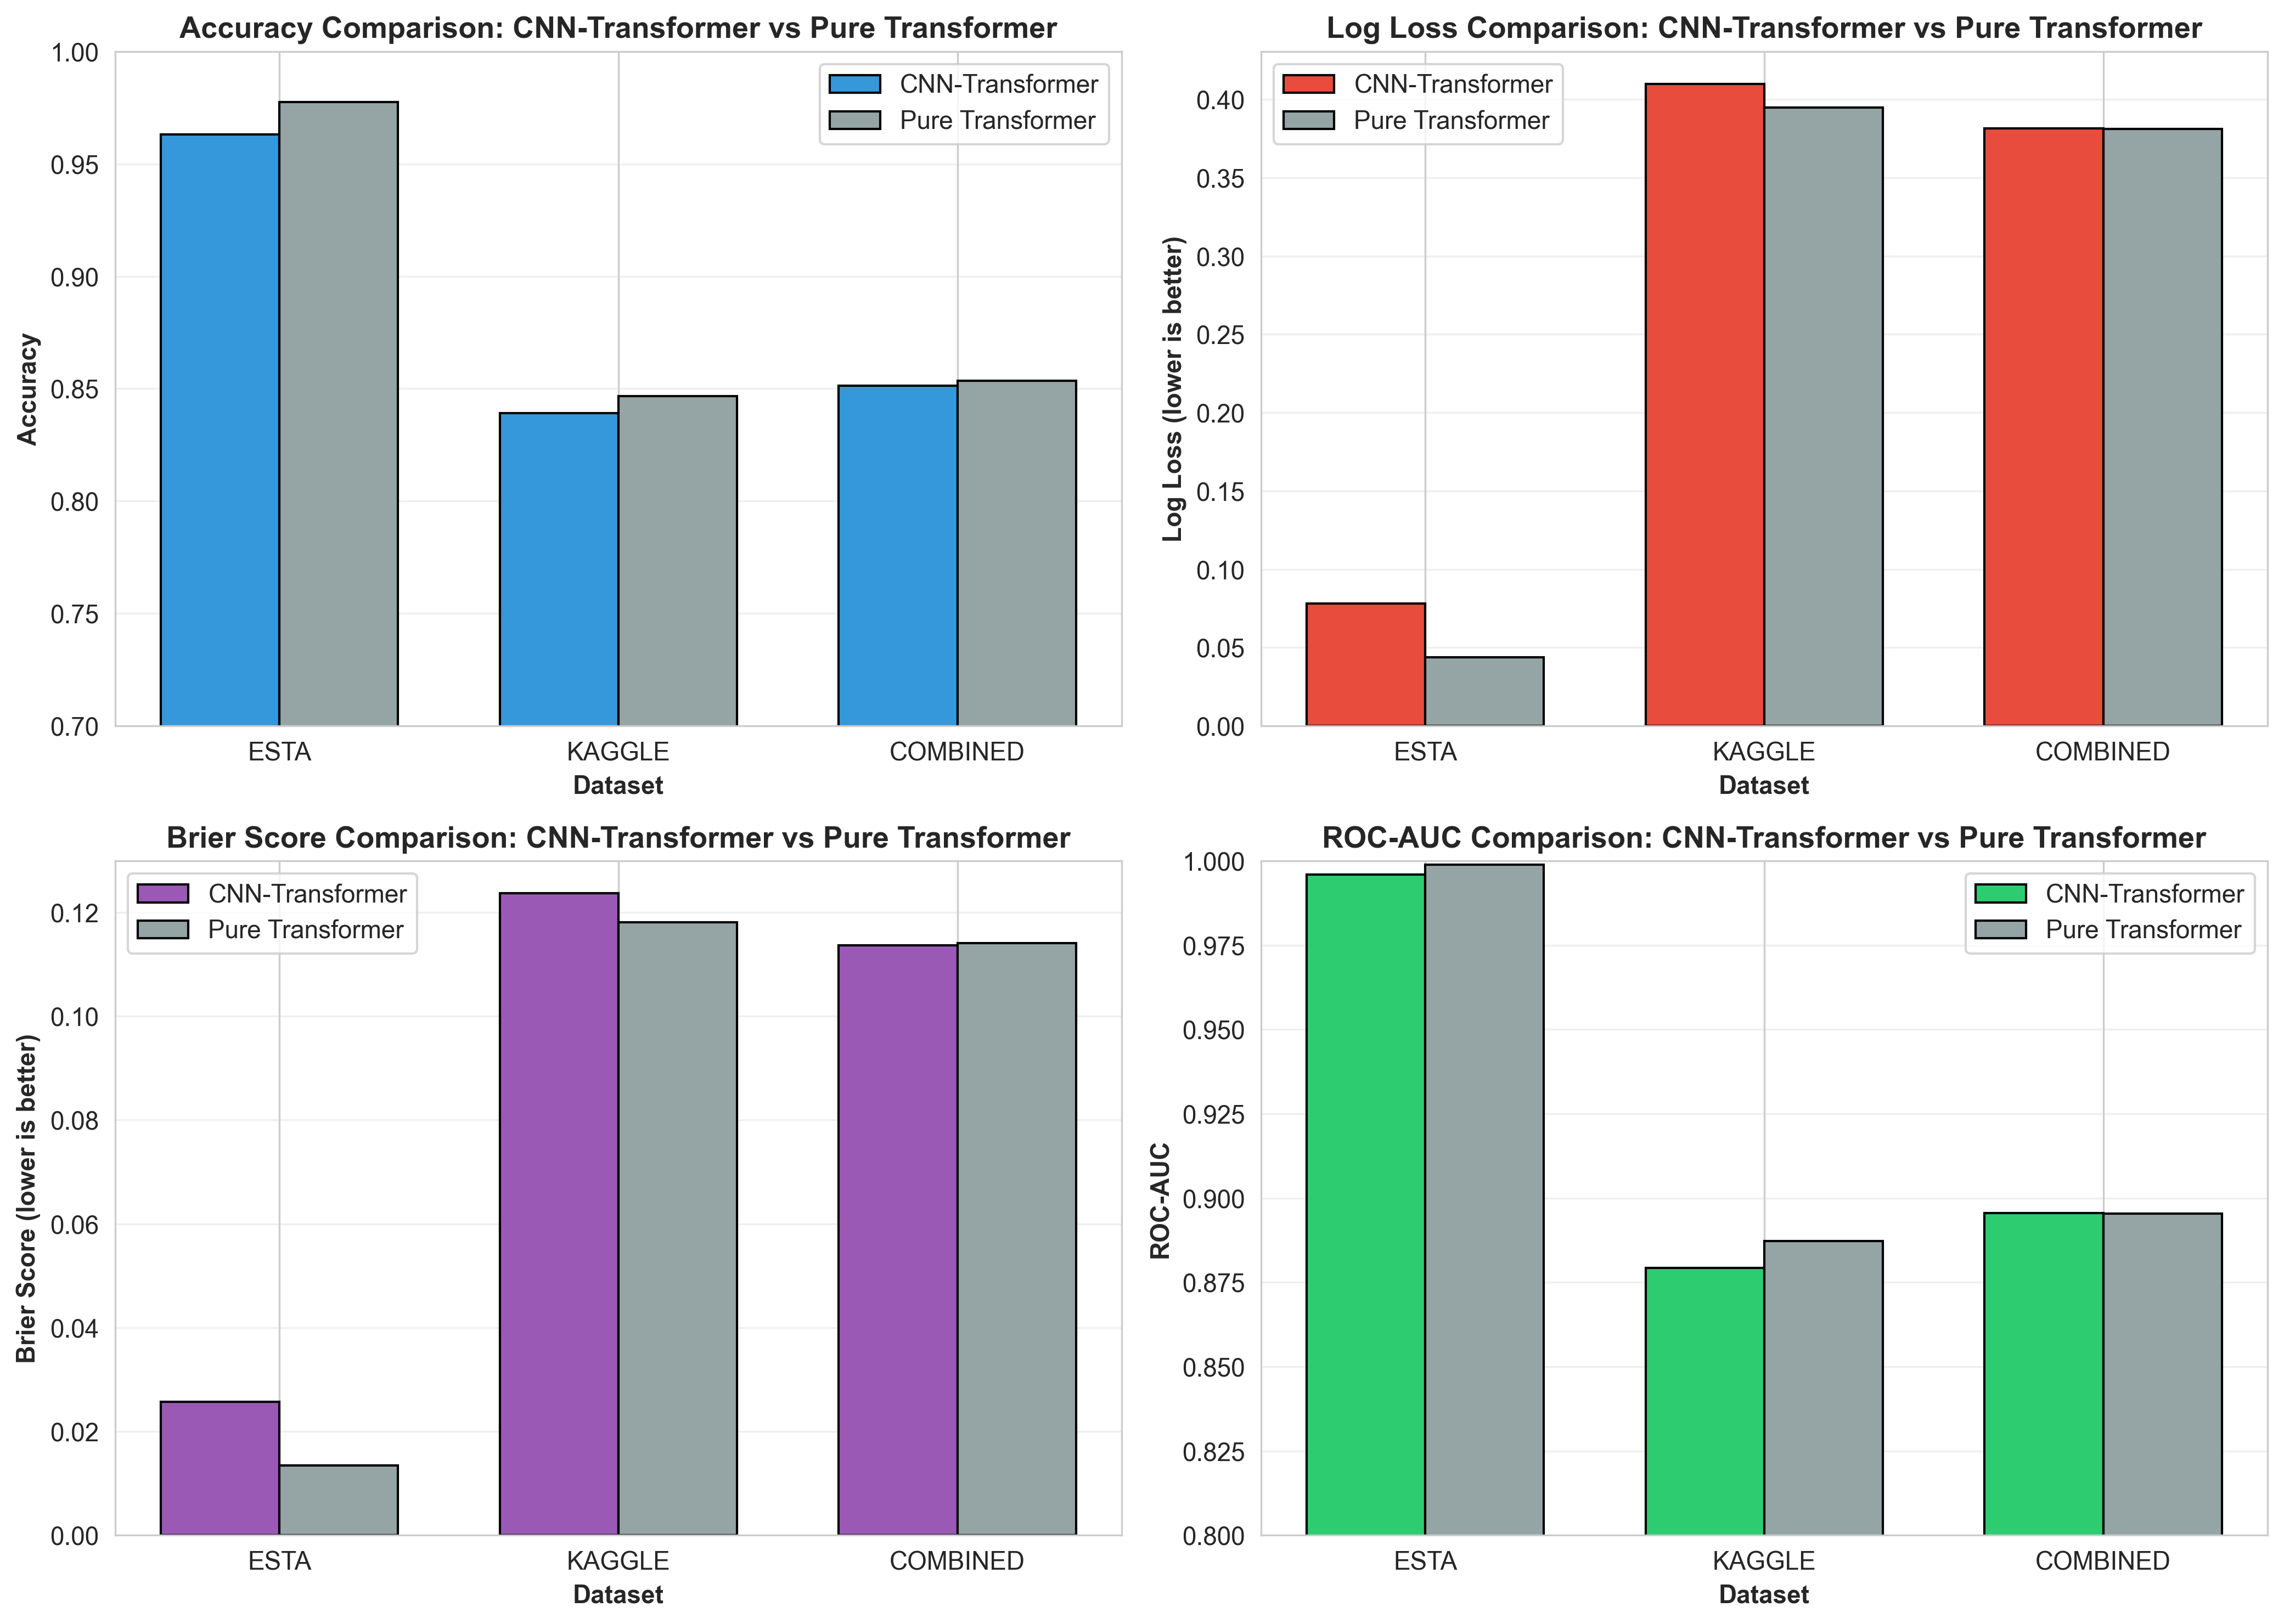
\includegraphics[width=0.9\textwidth]{results_analysis/results/cnn_transformer_figures/dataset_performance_comparison.png}
\caption{Dataset-specific performance comparison revealing different model behaviors across ESTA, Kaggle, and Combined datasets.}
\label{fig:dataset_comparison}
\end{figure}

\subsection{Recommendations}

Based on comprehensive empirical analysis:
\begin{enumerate}
    \item \textbf{Production Deployment:} Use the pure Transformer over the CNN-Transformer hybrid
    \item \textbf{Research Priority:} Add positional encodings to both architectures before pursuing additional complexity
    \item \textbf{Dataset-Specific Architecture:} If deploying on only ESTA, the CNN-Transformer's +0.8pp advantage may justify the instability cost
\end{enumerate}

\section{Conclusion}
\label{sec:conclusion}

\subsection{Summary of Contributions}

This project successfully developed and evaluated round-by-round win probability models for Counter-Strike:Global Offensive, addressing the research questions posed in the introduction.

\textbf{Key Contributions:}
\begin{enumerate}
    \item \textbf{Comprehensive benchmark:} Evaluated 4 models across 3 datasets at 7 checkpoint rounds
    \item \textbf{Economic insight:} Quantified the critical role of equipment values (42-49\% importance)
    \item \textbf{Calibration analysis:} Identified calibration trade-offs between accuracy and probability quality
    \item \textbf{Data quality validation:} Detected and documented severe data leakage in ESTA dataset
    \item \textbf{Ablation studies:} Demonstrated that scoreline alone achieves 67.5\% accuracy
\end{enumerate}

\subsection{Future Work}

\begin{itemize}
    \item Extension to CS2 (MR12 format) with updated mechanics
    \item Player-specific modeling (individual skill ratings)
    \item Map-specific strategy analysis
    \item Real-time prediction systems for live matches
    \item Causal analysis of economic decision impacts
\end{itemize}

\bibliographystyle{plain}
\begin{thebibliography}{99}

\bibitem{lock2014}
Lock, D., \& Nettleton, D. (2014). Using random forests to estimate win probability before each play of an NFL game. \textit{Journal of Quantitative Analysis in Sports}, 10(2), 197-205.

\bibitem{stern1994}
Stern, H. S. (1994). A Brownian motion model for the progress of sports scores. \textit{Journal of the American Statistical Association}, 89(427), 1128-1134.

\bibitem{yang2016}
Yang, P., Harrison, B. E., \& Roberts, D. L. (2016). Predicting match outcomes in League of Legends. In \textit{Twelfth Artificial Intelligence and Interactive Digital Entertainment Conference}.

\bibitem{hodge2019}
Hodge, V. J., Devlin, S., Sephton, N., Block, F., Drachen, A., \& Cowling, P. I. (2019). Win prediction in multiplayer esports: Live professional match prediction. \textit{IEEE Transactions on Games}.

\bibitem{agarwala2014}
Agarwala, A., \& Pearce, M. (2014). Learning dota 2 team compositions. Technical Report, Stanford University.

\bibitem{xenopoulos2020}
Xenopoulos, P., Doraiswamy, H., \& Silva, C. (2020). ESTA: A Platform for Esports Game Log and Replay Analysis. \textit{arXiv preprint arXiv:2011.01301}.

\bibitem{silva2017}
Silva, J. P., Sousa, T. A., \& Santos, D. S. (2017). Predicting the outcome of professional CS:GO matches. In \textit{International Conference on Entertainment Computing} (pp. 126-137).

\bibitem{vaswani2017}
Vaswani, A., Shazeer, N., Parmar, N., Uszkoreit, J., Jones, L., Gomez, A. N., ... \& Polosukhin, I. (2017). Attention is all you need. In \textit{Advances in neural information processing systems} (pp. 5998-6008).

\bibitem{fernandez2021}
Fernández, J., Bornn, L., \& Cervone, D. (2021). A framework for the fine-grained evaluation of the instantaneous expected value of soccer possessions. \textit{Machine Learning}, 110(6), 1389-1427.

\bibitem{decroos2019}
Decroos, T., Bransen, L., Van Haaren, J., \& Davis, J. (2019). Actions speak louder than goals: Valuing player actions in soccer. In \textit{Proceedings of the 25th ACM SIGKDD International Conference} (pp. 1851-1861).

\bibitem{pathak2020}
Pathak, N., \& Wadhwa, H. (2020). Applications of modern classification techniques to predict the outcome of ODI Cricket. \textit{Procedia Computer Science}, 87, 55-60.

\bibitem{he2015}
He, K., Zhang, X., Ren, S., \& Sun, J. (2015). Delving deep into rectifiers: Surpassing human-level performance on imagenet classification. In \textit{Proceedings of the IEEE international conference on computer vision} (pp. 1026-1034).

\bibitem{glorot2010}
Glorot, X., \& Bengio, Y. (2010). Understanding the difficulty of training deep feedforward neural networks. In \textit{Proceedings of the thirteenth international conference on artificial intelligence and statistics} (pp. 249-256).

\end{thebibliography}

\end{document}
